\documentclass[10pt,a4paper]{article}
\usepackage[utf8]{inputenc}
\usepackage[italian]{babel}
\usepackage{graphicx}
\usepackage{floatflt,epsfig}
\usepackage{graphicx}
\usepackage{pgfplots}
\usepackage{booktabs,xltabular}
\usepackage{amsmath}
\usepackage{tikz}
\usepackage{subcaption}
\usepackage{caption}
\usepackage{tabularx}
\usepackage{hyperref}
\usepackage{xcolor}
\hypersetup{
	colorlinks,
	linkcolor={red!50!black},
	citecolor={blue!50!black},
	urlcolor={blue!80!black}
}
\usepackage{pgfplots,pgfplotstable}
\usepackage{wrapfig}
\usepackage{float}
\usepackage{sidecap}
\bibliographystyle{plain}
\usepackage[export]{adjustbox}
\usepackage{xcolor}
\usepackage{listings}
\usepackage{amssymb}
\usepackage{amsmath,amssymb}
\usepackage{amscd} 
\usepackage{amsthm}
\usepackage{amssymb}
\usepackage{mathtools}

\lstset{language=Python,
basicstyle=\small,
keywordstyle=\color{black}\bfseries,
commentstyle=\color{orange},
numbers=left, numberstyle=\tiny, stepnumber=1, numbersep=5pt,
frame=single}

\title{Modello di ising 2D e transizione di fase}
\author{Francesco Anna Mele, Marco Eterno, Edoardo Maria Centamori}

\begin{document}
	\begin{titlepage}
		\begin{center}
			
			\vspace{1cm}
			{\LARGE\textbf{ Modello di ising 2D e transizione di fase}\par}
			
			\vspace{0.5cm}
			{\Large Francesco Anna Mele, Marco Eterno, Edoardo Maria Centamori\par}
			
			\vspace{1cm}
			
			
\includegraphics[width=0.4\linewidth]{unipi}
	
			
		\end{center}
	\end{titlepage}

\tableofcontents
\newpage
\section{Introduzione}
L'elaborato tratta la simulazione del \emph{modello di Ising classico} in 2 dimensioni su reticolo quadrato mediante l'\emph{algoritmo Metropolis}. Le proprietà termodinamiche di tale sistema sono note esattamente dalla soluzione analitica di Lars Osanger (1944). Tali proprietà verranno confrontate con quelle che ricaveremo numericamente.
%ANTICIPA LA LISTA DELLE COSE CHE ANALIZZIAMO NUMERICAMENTE
%\footnote{L. Onsager 1944, Phys. Rev. \textbf{65}, 117 (1944)}

\section{Modello di Ising classico bi-dimensionale}

Si consideri il \emph{modello di Ising classico} 2D su un reticolo quadrato $L \times L$. Ogni sito $i=(i_x,i_y)$ del reticolo rappresenta uno spin $s_i$ (che può assumere come valore $\pm 1$) con condizioni periodiche al bordo. Una configurazione $\sigma$ del sistema è definita dall'insieme dei valori degli spin del reticolo:
$$\sigma\coloneqq\{ s_i\text{ :}\text{ } i  \text{ è un sito del reticolo} \}$$
L'energia della configurazione $\sigma$ è data da:
\begin{equation}
E(\sigma)=-J\sum_{\langle i,j\rangle}s_i s_j-h\sum_{i}s_i
\label{eq:energia}
\end{equation}
dove la somma su $\langle i,j \rangle$ indica la somma sulle coppie di siti primi vicini, $J$ è l'accoppiamento tra i primi vicini e $h$ è il campo magnetico esterno uniforme.


All'equilibrio termico a temperatura $T$, la probabilità di avere la configurazione di spin $\sigma$ è data dalla distribuzione di Gibbs:
\begin{equation}
	P[\sigma]=\frac{1}{Z}e^{-\beta E(\sigma)}
	\label{eq:distribuzioneGibbs}
\end{equation}
dove 
$$\beta \coloneqq \frac{1}{kT}\text{ , }\qquad Z\coloneqq\sum_{\sigma}e^{-\beta E(\sigma)}$$
Se $J>0$, l'energia minore si raggiunge tramite allineamento degli spin in parallelo (in tal caso, si dice il sistema che ha un comportamento \emph{ferromagnetico}), altrimenti si raggiunge con gli spin in antiparallelo (comportamento \emph{antiferromagnetico}). In questo elaborato verrà analizzato il caso $J>0$. \\ 
Dato che nel seguito l'energia apparirà solo nell'esponenziale di Gibbs $e^{-\frac{E}{kT}}$,  possiamo sempre supporre $J=1$, a meno di ridefinire $T$ e $h$. Nell'elaborato verrà supposto sempre $h=0$. 
\section{Algoritmo}
L'algoritmo adottato per estrarre le configurazioni $\sigma$ secondo la distribuzione di probabilità $P[\sigma]$ è l'\emph{l'algoritmo Metropolis locale}. Tramite questo algoritmo si passa da una configurazione di spin di partenza a una configurazione di spin successiva modificando al più il valore dello spin di un solo sito del reticolo. Data una qualsiasi configurazione iniziale, dopo un numero sufficiente di applicazioni dell'algoritmo (detto \emph{tempo di autocorrelazione esponenziale} o \emph{tempo di termalizzazione}), si ottiene la configurazione $\sigma$ con probabilità $P[\sigma]$.

Di seguito vengono riportati i passi dell'algoritmo. Si supponga che la configurazione iniziale sia $\sigma=\{ s_i\text{ :}\text{ } i  \text{ è un sito del reticolo} \}$.

\begin{itemize}
	\item \emph{Passo 1}: Si seleziona un sito $i_0$ in modo casuale. 
	
	Definiamo $\sigma_{try}$ come: $$\sigma_{try}\coloneqq\{ \tilde{s}_i\text{ :}\text{ } i  \text{ è un sito del reticolo} \}$$ 
	\begin{equation*}
	\tilde{s}_{i}\coloneqq
	\begin{cases}
	-s_{i_0} & \text{ se $i= i_0 $,	} \\
	s_i & \text{ altrimenti}
	\end{cases}
	\end{equation*}
	Inoltre definiamo $r$ come:
	$$r\coloneqq \frac{P[\sigma_{try}]}{P[\sigma]}$$
	e usando le equazioni \ref{eq:energia} e \ref{eq:distribuzioneGibbs} si ottiene:
	$$r=\exp\left[-2\beta s_{i_0}\left(\sum_{i\in\text{p.v.}i_0}s_i+h\right)\right]$$
	dove $\text{p.v.}i_0$ indica l'insieme dei siti primi vicini del sito $i_0$.
	\item \emph{Passo 2}: Si estrae un numero $x$ casuale tra $0$ e $1$. Se $x<r$ la configurazione finale diventa $\sigma_{try}$, altrimenti resta $\sigma$.
\end{itemize}
Nel codice utilizzato viene definita la funzione \emph{update\_metropolis} che itera $L^2$ volte l'algoritmo metropolis locale (ciò corrisponde ad una "spazzata" del reticolo). 
\subsection{Strategia di campionamento e linguaggi di programmazione utilizzati}
Il codice che campiona le storie montecarlo (cioè energia e magnetizzazione in funzione del tempo montecarlo) è stato implementato in C. Dopo aver ottenuto i files di storie montecarlo per ogni valore di $L$ e $\beta$ desiderato, un codice scritto in Python si occupa di tutta l'analisi dati (compreso il calcolo delle osservabili e l'errore associato)\footnote{In questo modo, osservabili diverse si possono calcolare a partire dalla stessa storia montecarlo. Questo è sicuramente più efficiente rispetto a calcolare le osservabili e le storie montecarlo contemporaneamente (che richiederebbe una simulazione diversa per ogni osservabile)}.


Prima di iniziare a campionare le storie montecarlo, abbiamo chiamato la funzione \emph{update\_metropolis} un numero sufficientemente elevato di volte in modo da essere sicuri che il sistema termalizzasse. Inoltre, come verrà spiegato nel paragrafo \ref{Campionamento}, abbiamo adottato una strategia che permette di ridurre i tempi di termalizzazione.



Come esempio di termalizzazione, nelle figure \ref{term035} e \ref{term045} vengono riportate le storie montecarlo della magnetizzazione per reticolo di lato $L=50$ rispettivamente per $\beta=0.35$ e per $\beta=0.45$. Il sistema impiega un opportuno numero di step montecarlo per termalizzare. Tale numero di step dipende sia dalla temperatura sia dalla grandezza del reticolo.\footnote{Il tempo di termalizzazione aumenta sia all'aumentare di $L$ e sia avvicinandosi alla temperatura critica. Questo è in accordo con quello che si osserva dalle figure \ref{term035} e \ref{term045}: si vede che il tempo di termalizzazione relativo a $\beta=0.45$ è maggiore rispetto a quello relativo a $\beta=0.35$. Questo è consistente con il fatto che $\beta=0.45$ è più vicino alla temperatura critica.}
\begin{figure}[h!]%prodotti da magn_step.c e vedere cartella StoriamONTEcARLO
	\centering
	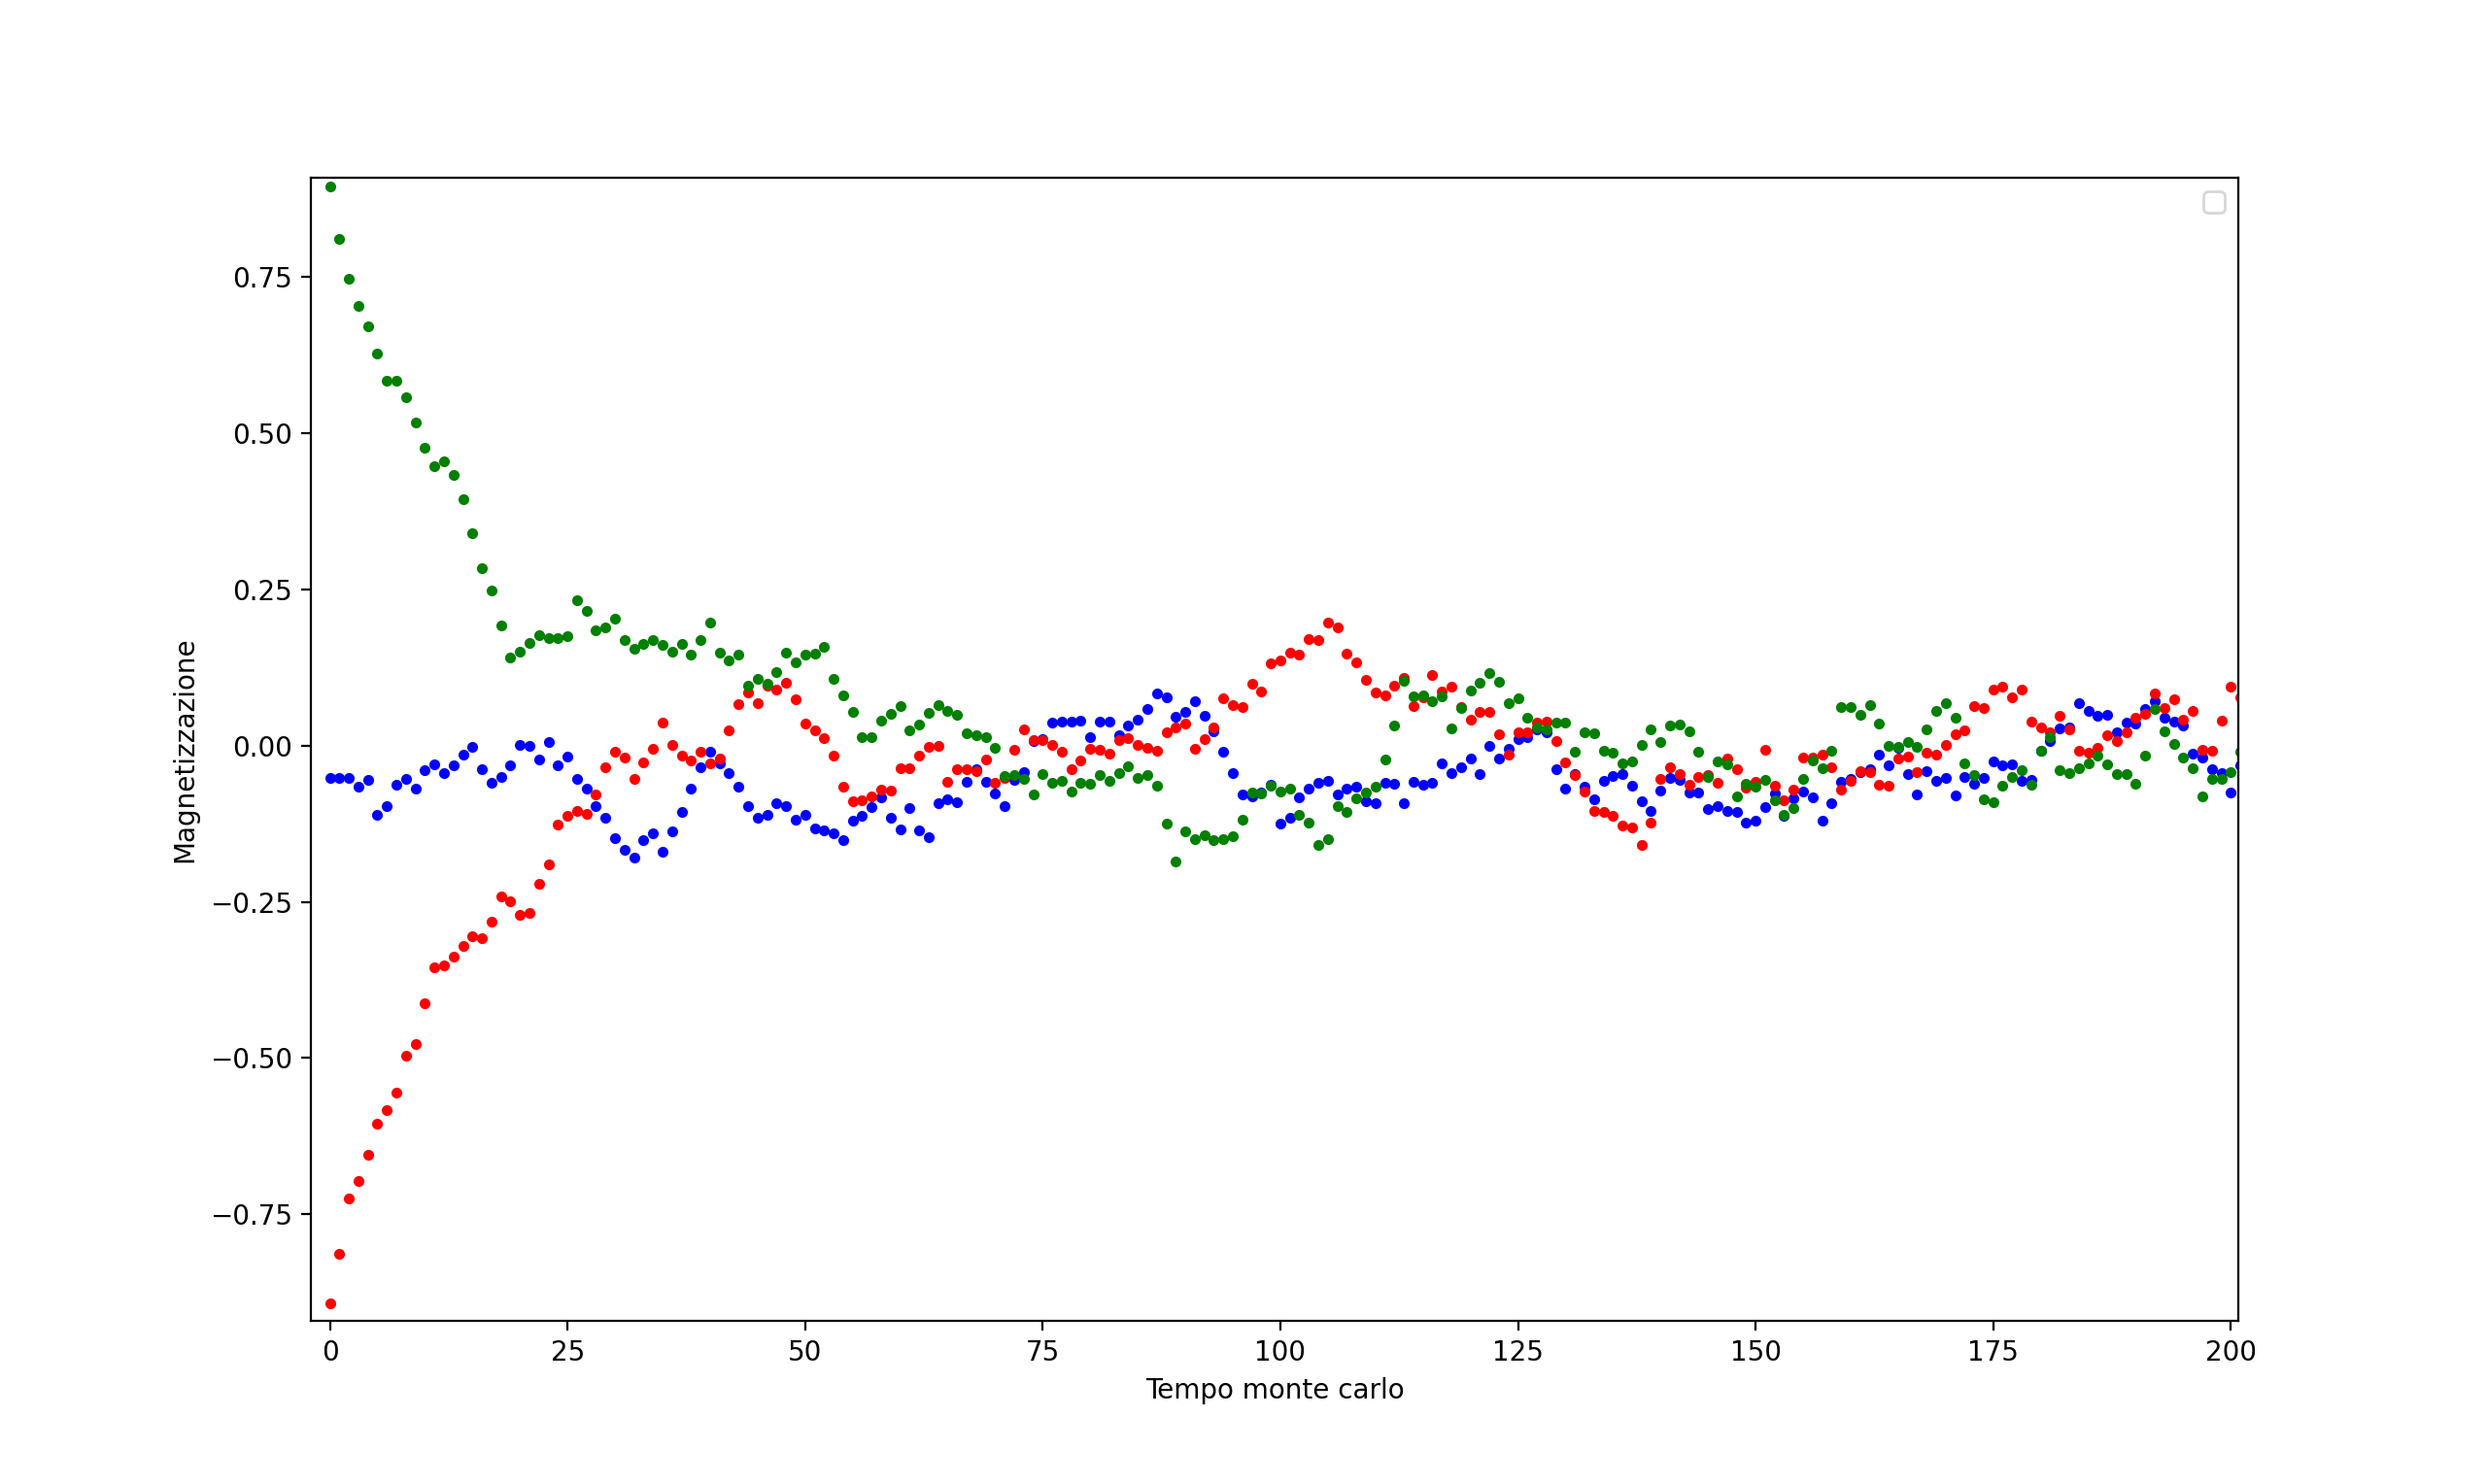
\includegraphics[width=0.90\linewidth]{term035}
	\caption{Magnetizzazione a temperatura $\beta=0.35$ per $L=50$ in funzione del tempo montecarlo. Uno step di tempo montecarlo corrisponde ad una chiamata della funzione update\_metropolis. I punti verdi corrispondono alla configurazione iniziale in cui tutti gli spin valgono $+1$, i punti blu corrispondono alla configurazione iniziale in cui gli spin sono $+1$ o $-1$ in modo random, i punti rossi alla configurazione iniziale in cui tutti gli spin valgono $-1$. Il sistema termalizza dopo circa $\sim 60$ step montecarlo.}
	\label{term035}
\end{figure}

\begin{figure}[h!]
	\centering
	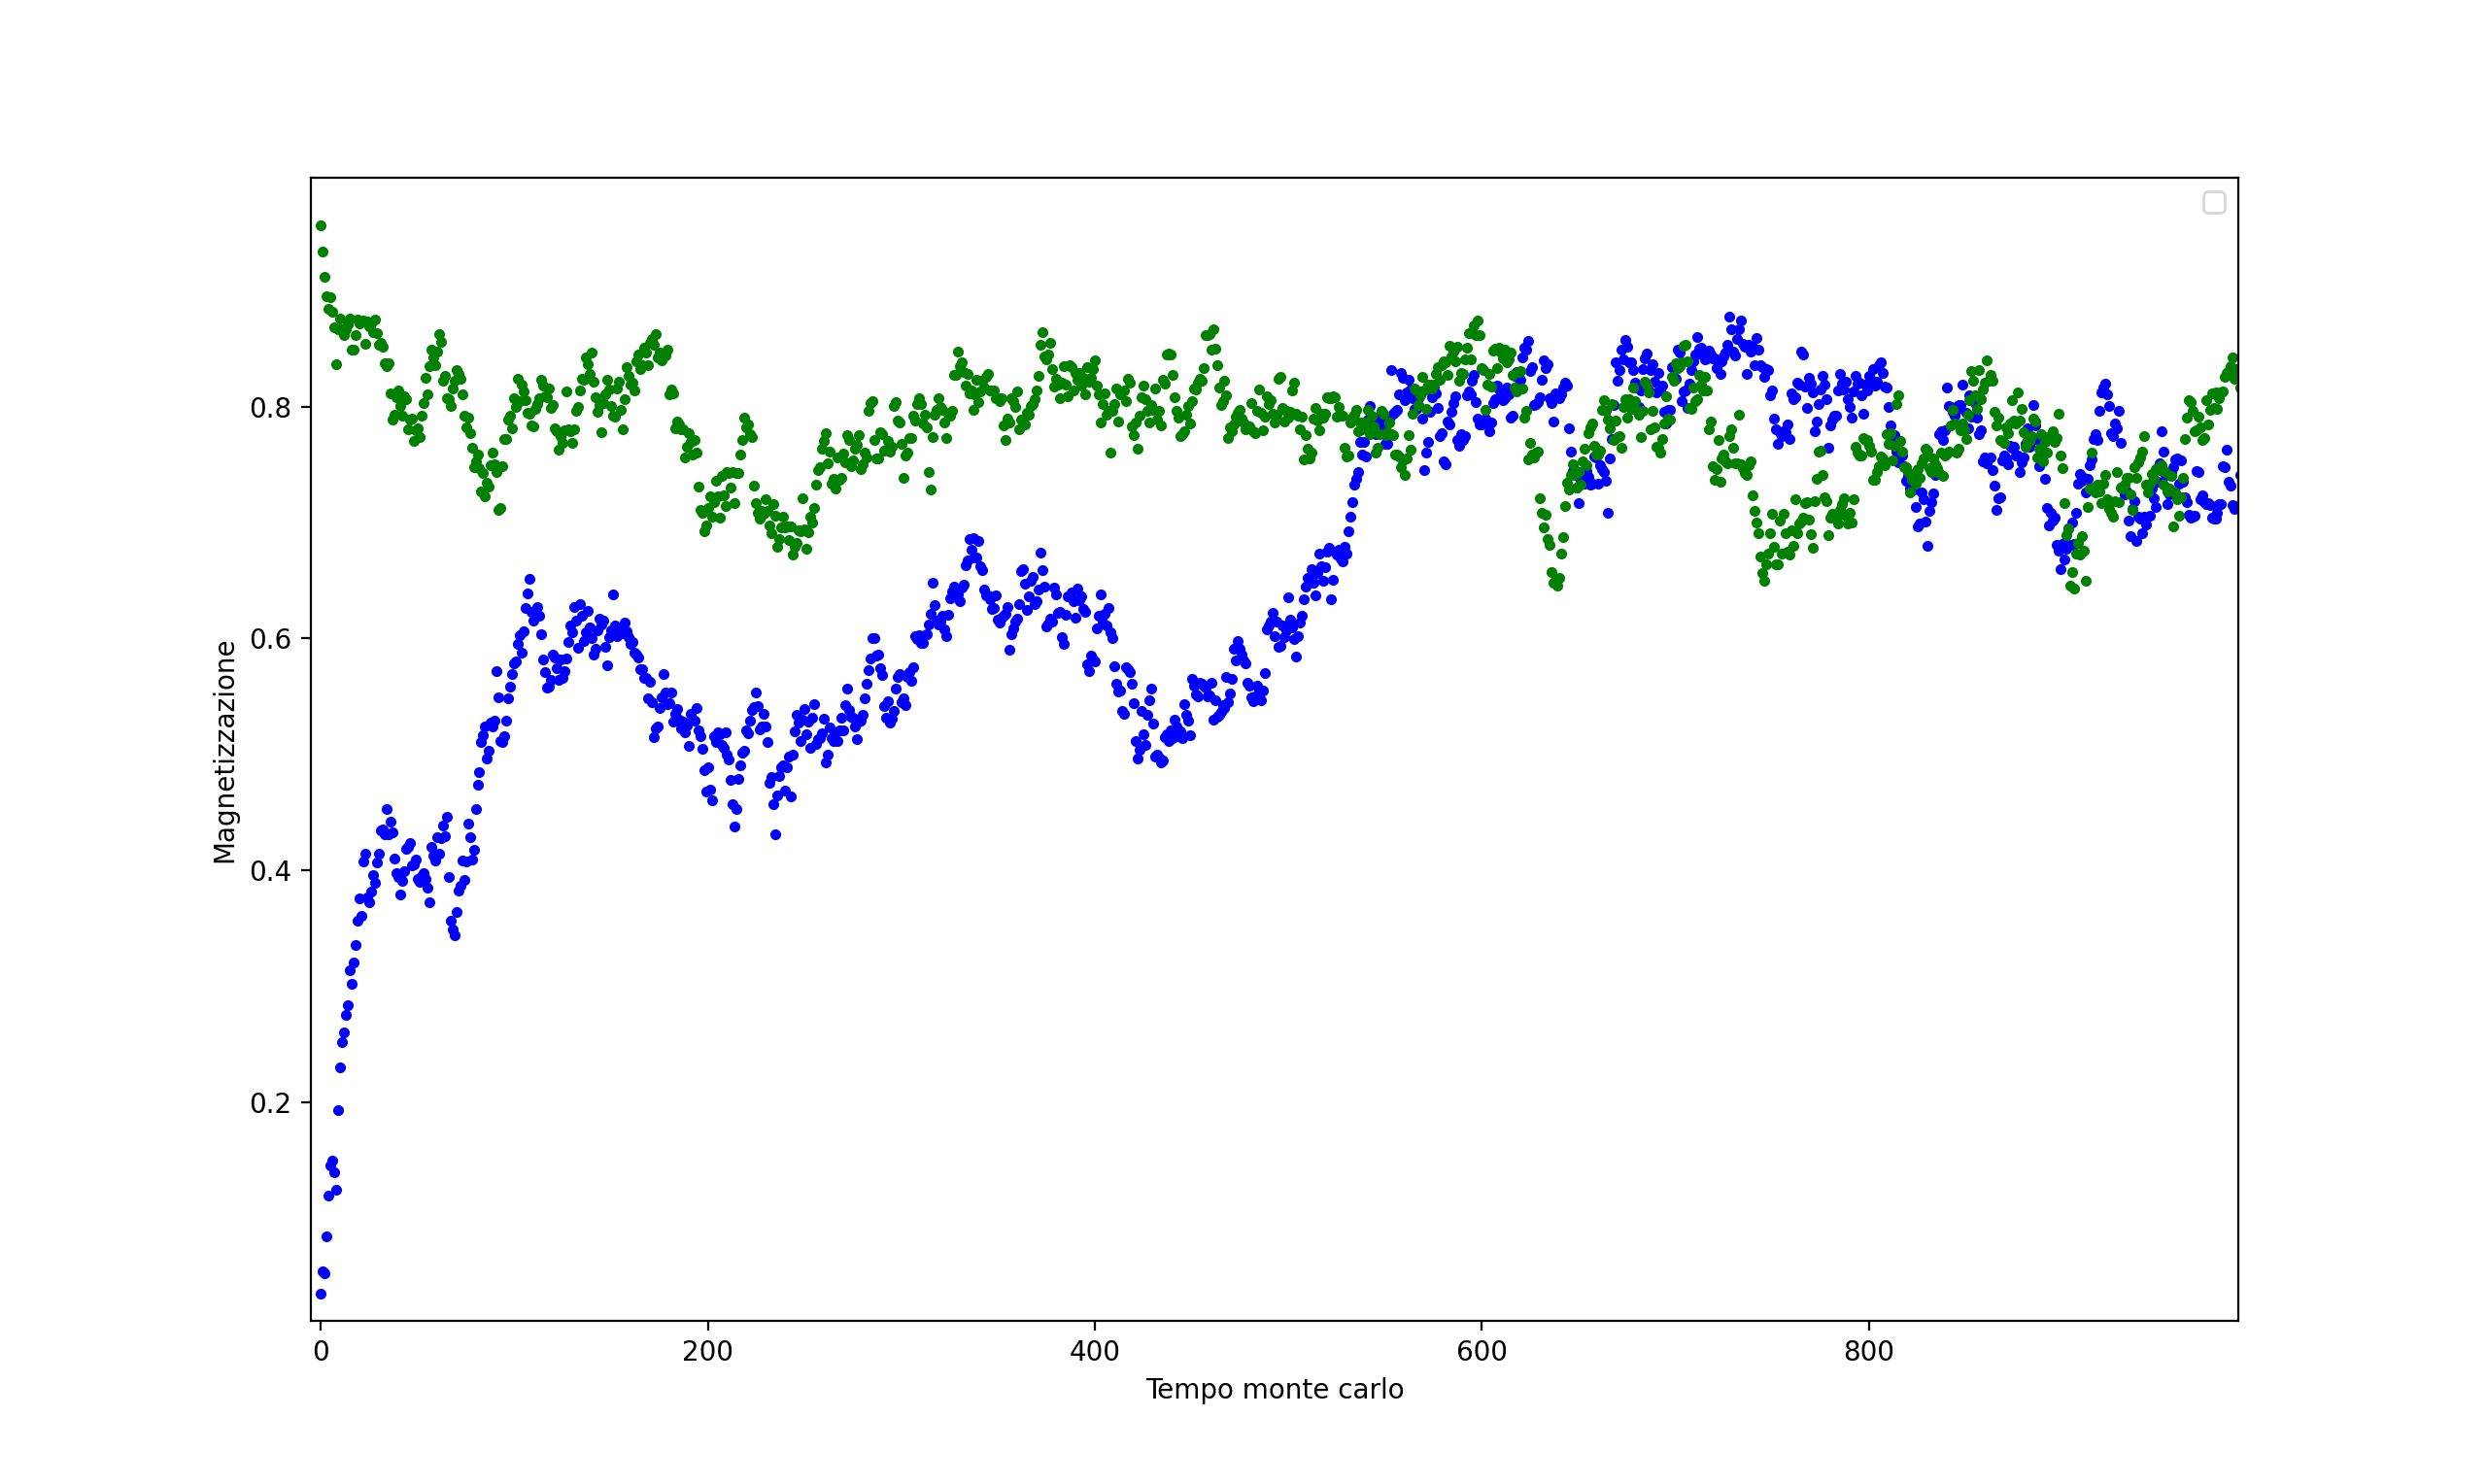
\includegraphics[width=0.90\linewidth]{term045}
	\caption{Magnetizzazione a temperatura $\beta=0.45$ per $L=50$ in funzione del tempo montecarlo. Uno step di tempo montecarlo corrisponde ad una chiamata della funzione update\_metropolis.  I punti verdi corrispondono alla configurazione iniziale in cui tutti gli spin valgono $+1$, i punti blu corrispondono alla configurazione iniziale in cui gli spin sono $+1$ o $-1$ in modo random. Il sistema termalizza dopo circa $\sim 600$ step montecarlo.}
	\label{term045}
\end{figure}

%Idea: per sconfiggere il tempo di termalizzazione si può adottare la seguente strategia.  Quando si varia beta di poco, si può misurare l'osservabile in questione con il nuovo beta partendo dall'ultima configurazione ottenuta con il vecchio beta.


\newpage

\section{Parametri d'ordine}
Sia $\mathbf{Z_2}$ il gruppo formato dalle trasformazioni "\emph{identità}" e "\emph{inversione degli spin}". Quest'ultima trasformazione agisce sulla configurazione $\sigma$ come:\begin{center}
	$\sigma=\{ s_i  : i $ è un sito del reticolo$ \}$ $\longrightarrow$ $\sigma'\coloneqq\{ - s_i  : i $ è un sito del reticolo$ \}$
\end{center} 
Se il campo magnetico $h$ è nullo, il sistema è invariante sotto $\mathbf{Z_2}$. Infatti, risulta: $$E(\sigma)=E(\sigma')\text{ .}$$
Si vuole analizzare l'esistenza di una \emph{temperatura critica} $T_c\ne 0$ tale che al di sotto si abbia una \emph{rottura spontanea} della simmetria $\mathbf{Z_2}$. 

Per analizzare il sistema è utile introdurre un \emph{parametro d'ordine}, ovvero una quantità che permette di capire se vi è o non vi è rottura spontanea di simmetria. Un esempio è la \emph{magnetizzazione} $M(\sigma)$:
\begin{equation}
	M(\sigma)\coloneqq\frac{1}{L^2}\sum_{i}s_i
	\label{eq:magn}
\end{equation}
Se la media sulla distribuzione di Gibbs della magnetizzazione è nulla, ovvero $\langle M \rangle $ $=0$, la simmetria è non rotta. Se invece $\langle M \rangle $ $\ne 0$, è presente rottura spontanea di simmetria.\\
Dalla soluzione analitica di Osanger, risulta che la transizione di fase tra fase rotta e fase non rotta avviene ad una temperatura $T_c$ pari a (usando unità $k=1$):
\begin{equation}
\beta_c=\frac{1}{T_c}=\frac{\ln(1+\sqrt{2})}{2}= 0.4406868\text{...}
\label{eq:temperatura-critica}
\end{equation}
detta \emph{temperatura critica} (o anche \emph{Temperatura di Curie}).\\
Per $T<T_c$, la magnetizzazione media assume un valore diverso da $0$. \\
Alla temperatura critica il valor medio di M tende a zero, ovvero la transizione di fase è una \emph{transizione continua} (detta anche \emph{transizione del secondo ordine}). Questi risultati valgono nel limite $L\rightarrow \infty$. Nel paragrafo successivo viene considerato il caso in cui $L$ è finito, che è il caso con cui si ha a che fare in un'analisi numerica.
%Inserire qui eventualmente la spiegazione dell'algoritmo
\subsection{Magnetizzazione media nulla per reticolo finito}
Si osserva che:
\begin{center}
	\emph{Se il reticolo è finito, il valor medio della magnetizzazione è nullo per ogni valore di $\beta$.}
\end{center}
Ciò è stato verificato numericamente plottando la magnetizzazione in funzione del tempo montecarlo, come mostrato in figura \ref{fig:magnstepbeta045} e in figura \ref{fig:magnstepbeta035}. In queste figure, uno step di tempo montecarlo corrisponde a $100$ spazzate del reticolo con l'algoritmo Metropolis. %Vedere programma magn_step.c e cartella magn_stepFile
\begin{figure}[h!]
	\centering
	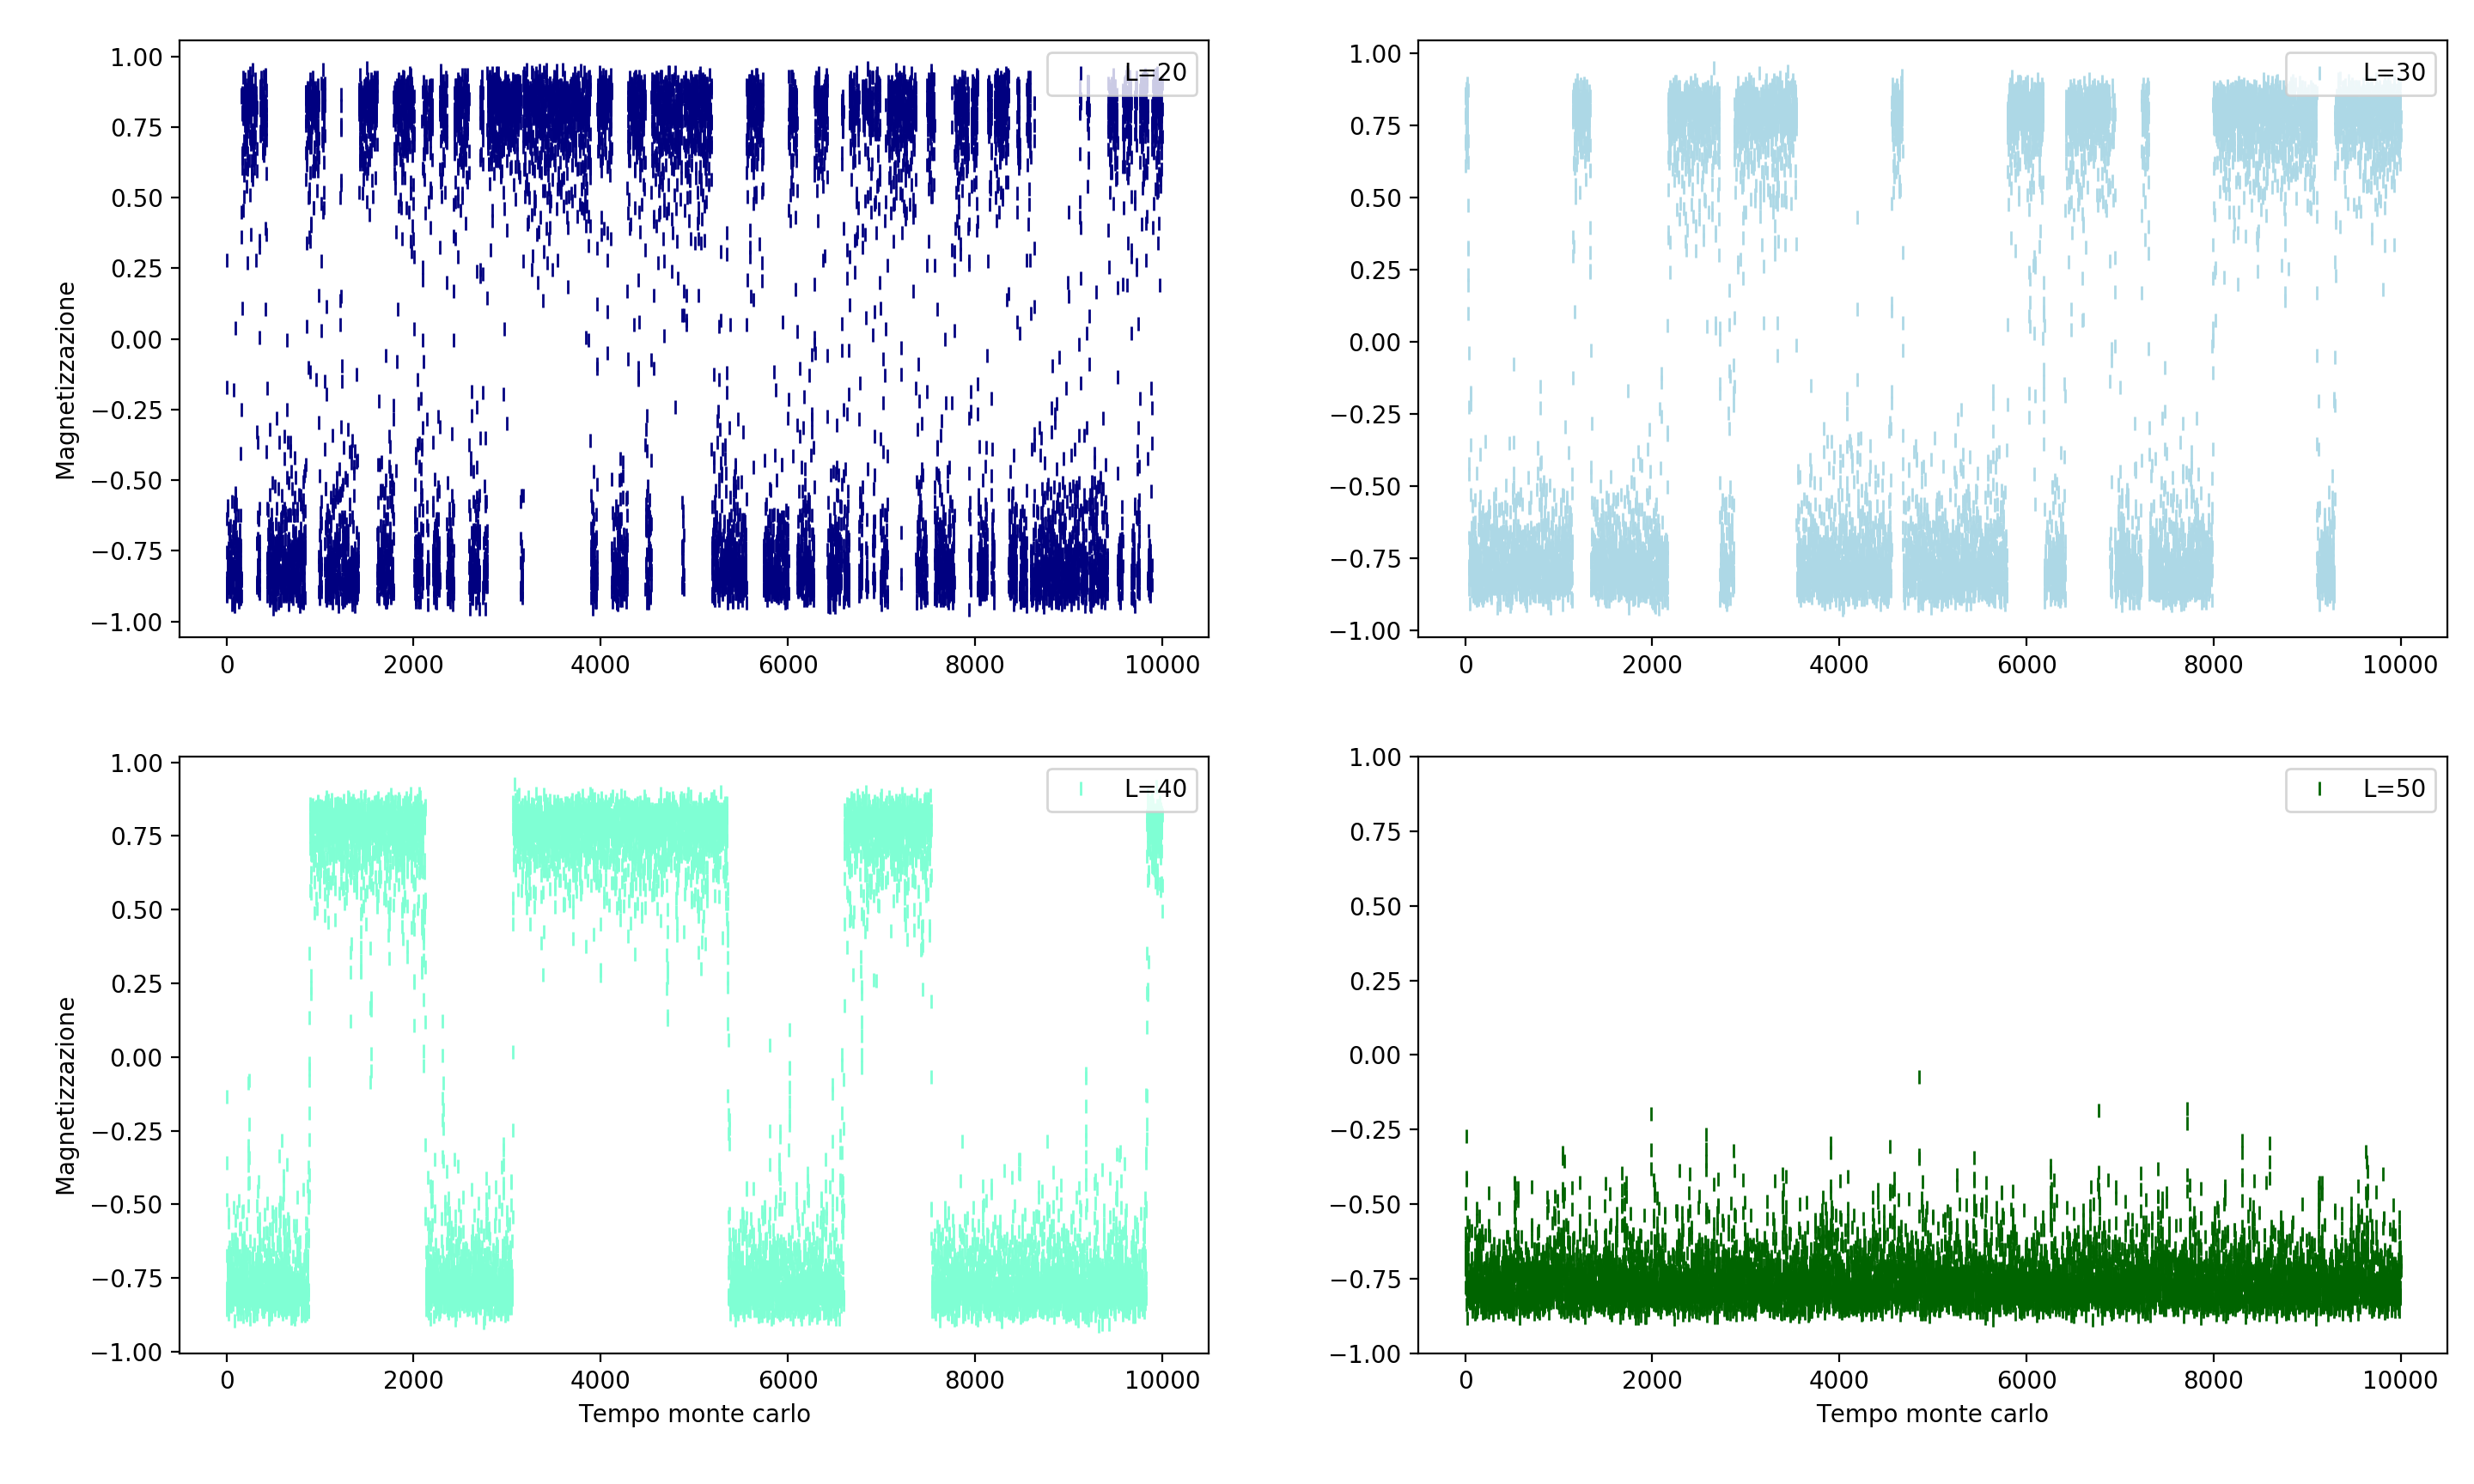
\includegraphics[width=1\linewidth]{magn_step_beta045rinnovo}
	\caption{Magnetizzazione a temperatura $\beta=0.45$ per i valori di $L=$ 20, 30, 40 e 50. Ogni punto del grafico è stato calcolato ogni $100$ chiamate della subroutine \emph{update\_metropolis} (che implementa una spazzata del reticolo con l'algoritmo Metropolis). Si osservi che all’aumentare di $L$ le variazioni di segno di $M$ sono sempre più rare. Per $L=50$ non si osserva variazione di segno della magnetizzazione in quanto la storia Monte Carlo è troppo corta.}
	\label{fig:magnstepbeta045}
\end{figure}

\begin{figure}[h!]
	\centering
	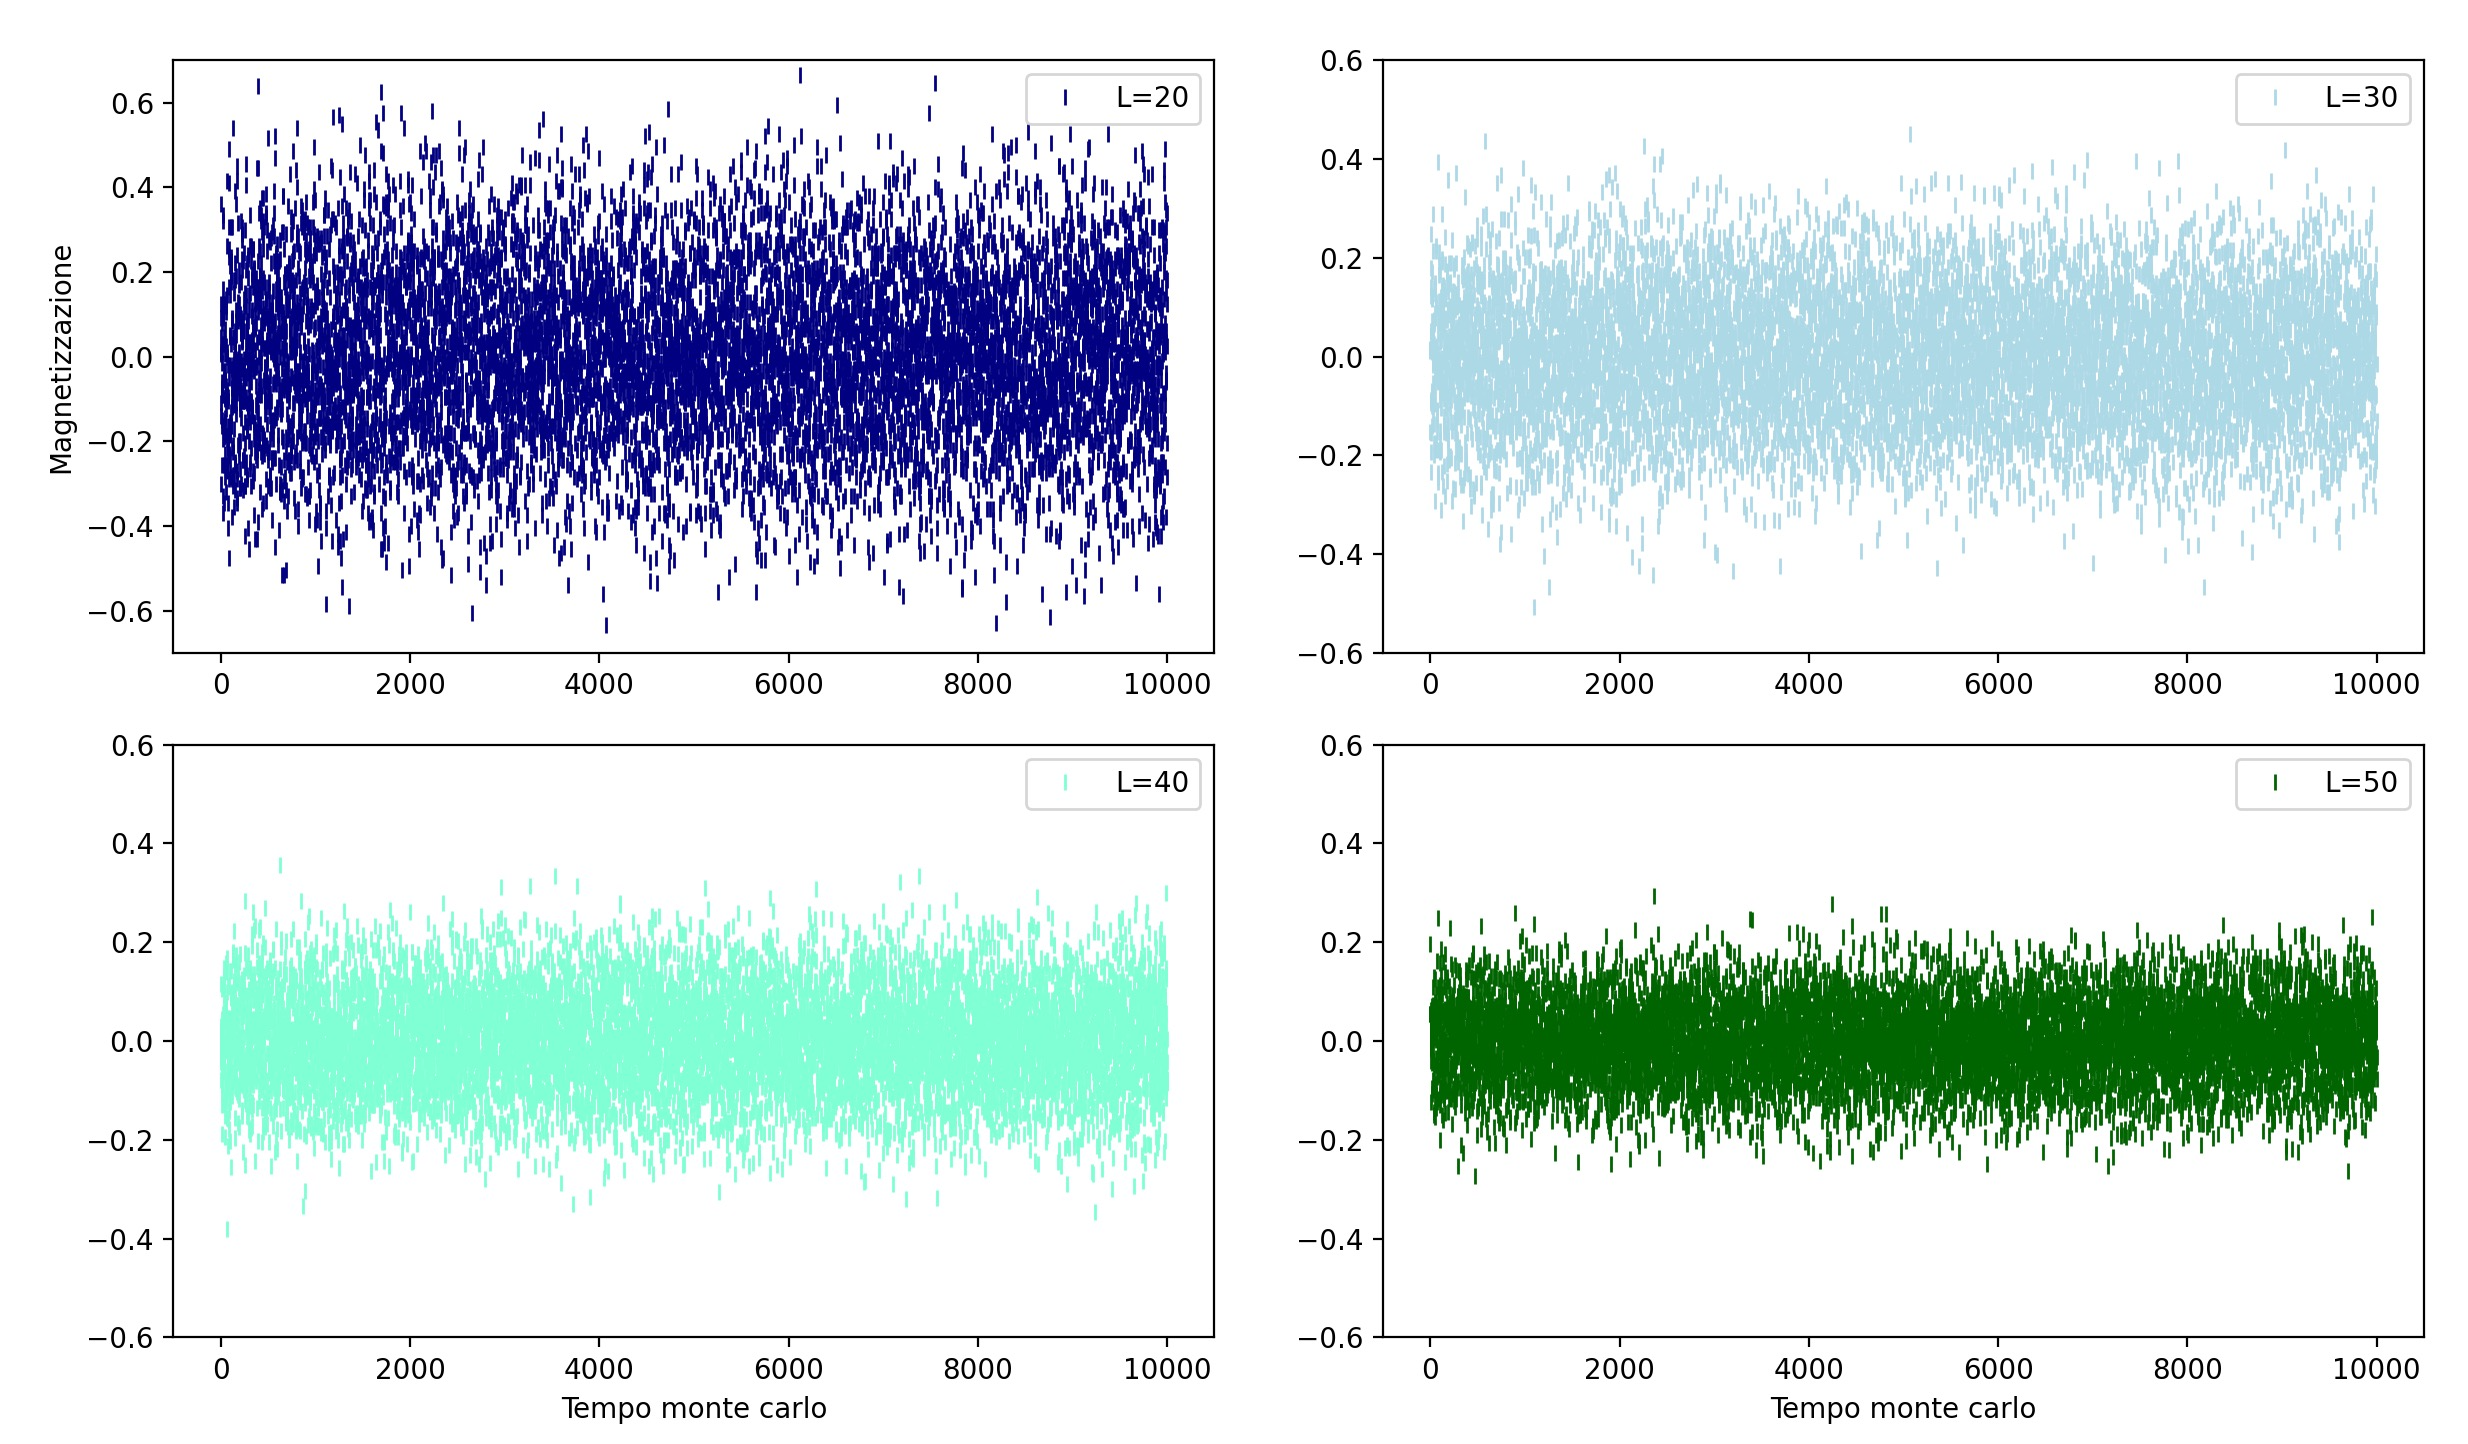
\includegraphics[width=1\linewidth]{magn_step_beta035}
	\caption{Magnetizzazione a temperatura $\beta=0.35$ per i valori di $L=$ 20, 30, 40 e 50. Ogni punto del grafico è calcolato ogni $100$ chiamate della subroutine \emph{update\_metropolis}. Si osservi che all'aumentare di $L$, la varianza di $M$ è sempre più piccola.}
	\label{fig:magnstepbeta035}
\end{figure}

Sotto la temperatura critica, sebbene aumentando $L$ la magnetizzazione passa sempre più raramente da un valore $m\ne0$ al valore $-m$, esisterà sempre un tempo montecarlo sufficientemente grande dopo il quale il sistema riesca a far cambiare segno alla magnetizzazione. Questo andamento è evidente nella figura \ref{fig:magnstepbeta045}. Per $L\rightarrow\infty$, invece, la magnetizzazione media resta fissata ad un valore diverso da $0$: questo è il fenomeno della \emph{rottura spontanea di simmetria}.

%spiegare perché cambia  MEGLIO 
Per questo motivo, a livello numerico (e quindi per $L$ finito), non va bene utilizzare la magnetizzazione media come parametro d'ordine. 


\subsection{Cumulante di Binder}
Un modo per comprendere se si è nella fase di simmetria rotta o nella fase di simmetria non rotta è analizzare la \emph{distribuzione di probabilità della magnetizzazione} $P(M)$:
\begin{itemize}
	\item Per $T<T_c$ :\\
	$P(M)$ è una distibuzione simmetrica con due picchi. Nel limite di $L\rightarrow \infty$ si ha:
	\[
		P(M)=\frac{1}{2}\left(\delta(M-m)+\delta(M+m)\right) \quad \mathrm{con} \quad m=\lim_{L\to\infty} \langle |M| \rangle
	\]
	Al crescere di $L$, la probabilità che il sistema salti da un valore di magnetizzazione $+m$ a un valore $-m$ tende a zero.
	\item Per $T>T_c$ :\\
	$P(M)$ è una gaussiana centrata in $M=0$ con larghezza che tende a $0$ come $1/L$ nel limite termodinamico $L\to\infty$. 
\end{itemize}
Come esempio, in figura \ref{istogramma} sono riportate le distribuzioni campionarie della magnetizzazione ottenute con un reticolo di lato $L=40$ alle temperature $\beta=0.45$ e $\beta=0.35$.
\begin{figure}[h!]
	\centering
	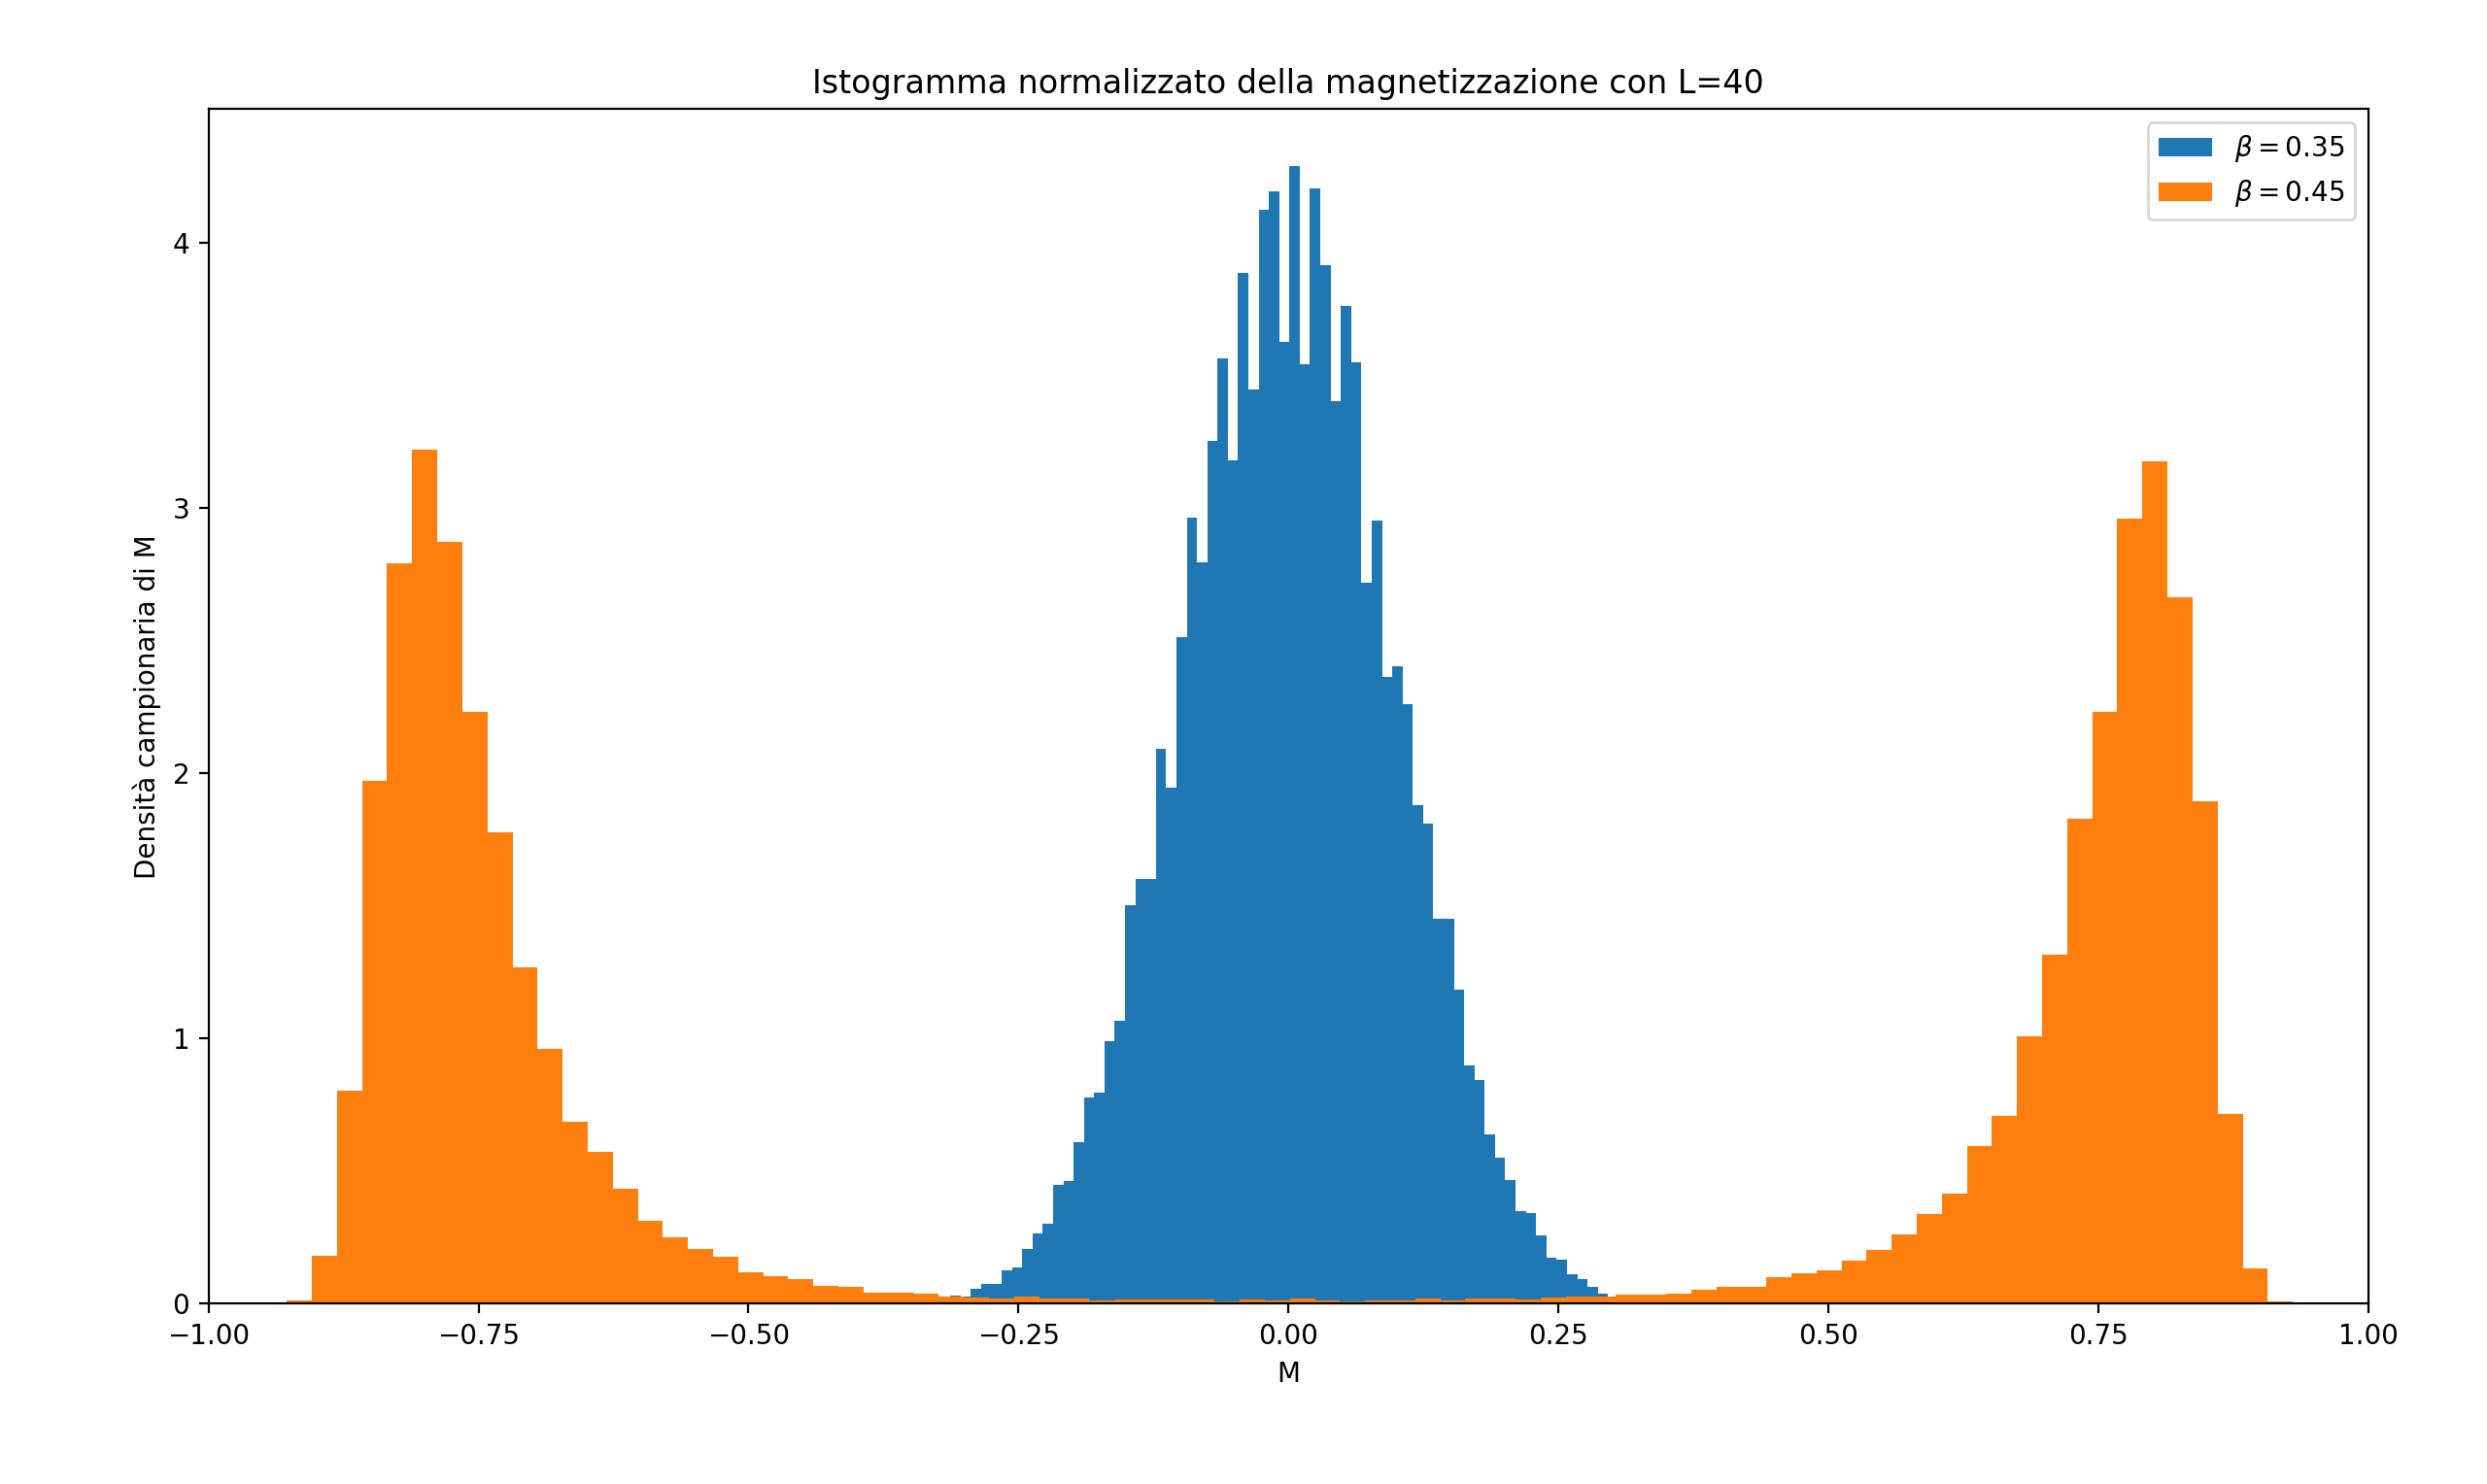
\includegraphics[width=1\linewidth]{istogramma}
	\caption{Istogrammi normalizzati della magnetizzazione su reticolo di lato $L=40$ alle temperature $\beta=0.45$ e $\beta=0.35$. I due istogrammi sono costruiti con i dati della magnetizzazione graficati in figura \ref{fig:magnstepbeta045} e \ref{fig:magnstepbeta035}.}
	\label{istogramma}
\end{figure}


 Il problema si sposta, dunque, nel calcolare un'osservabile che permette di determinare se la distribuzione $P(M)$ è una gaussiana oppure una somma di due delte di Dirac. A tale scopo, definiamo il \emph{cumulante di Binder} $B$:
\begin{equation}
	B\coloneqq\frac{\langle M^4\rangle}{\langle M^2\rangle ^2}
\end{equation}
Per $L\to\infty$, il cumulante di Binder soddisfa la seguente proprietà:
\begin{equation}\label{BinderTc}
B=
\begin{cases}
1 & \text{ se $T< T_c $,	} \\
3 & \text{ altrimenti}
\end{cases}
\end{equation}

Il valore del cumulante di Binder $B$, perciò, caratterizza la situazione in cui si è ad una temperatura maggiore o minore della temperatura critica.

Teoricamente, sappiamo che $\beta=0.35$ e $\beta=0.45$ corrispondono ad una temperatura rispettivamente maggiore e minore della temperatura critica. Questo è quello che andremo a verificare numericamente calcolando il cumulante di Binder.


In figura \ref{binder035} e \ref{binder045} vengono riportati i valori ottenuti del cumulante di Binder al variare di $L$ rispettivamente per $\beta=0.35$ e per $\beta=0.45$. Ogni valore del cumulante di Binder riportato nelle figure \ref{binder035} e \ref{binder045} è stato ottenuto a partire da $30000$ misure di magnetizzazione. Ogni misura di magnetizzazione è stata presa dopo 100 chiamate della subroutine update\_metropolis. L'errore è stato stimato con il metodo \emph{bootstrap con binning}. I dettagli di tale stima sono riportati nel paragrafo \ref{ParErrBinder}. Inoltre, per ridurre il tempo di termalizzazione, per $\beta=0.35$ è stata scelta la configurazione iniziale in cui ogni spin è $+1$ o $-1$ in modo random, mentre per $\beta=0.45$ è stata scelta la configurazione iniziale in cui tutti gli spin sono $+1$.
\begin{itemize}
	\item \emph{Caso} $\beta=0.35$ :\\
	Dalla figura \ref{binder035} (che si riferisce al caso $\beta=0.35$) si osserva che $B$ tende a $3$ per $L$ sufficientemente grande, il che rispetta le aspettative per una temperatura maggiore della temperatura critica (equazione \ref{BinderTc}). 
	%allegare referenza per questo andamento
	\begin{figure}[h!]%vedere programma binder.c
		\centering
		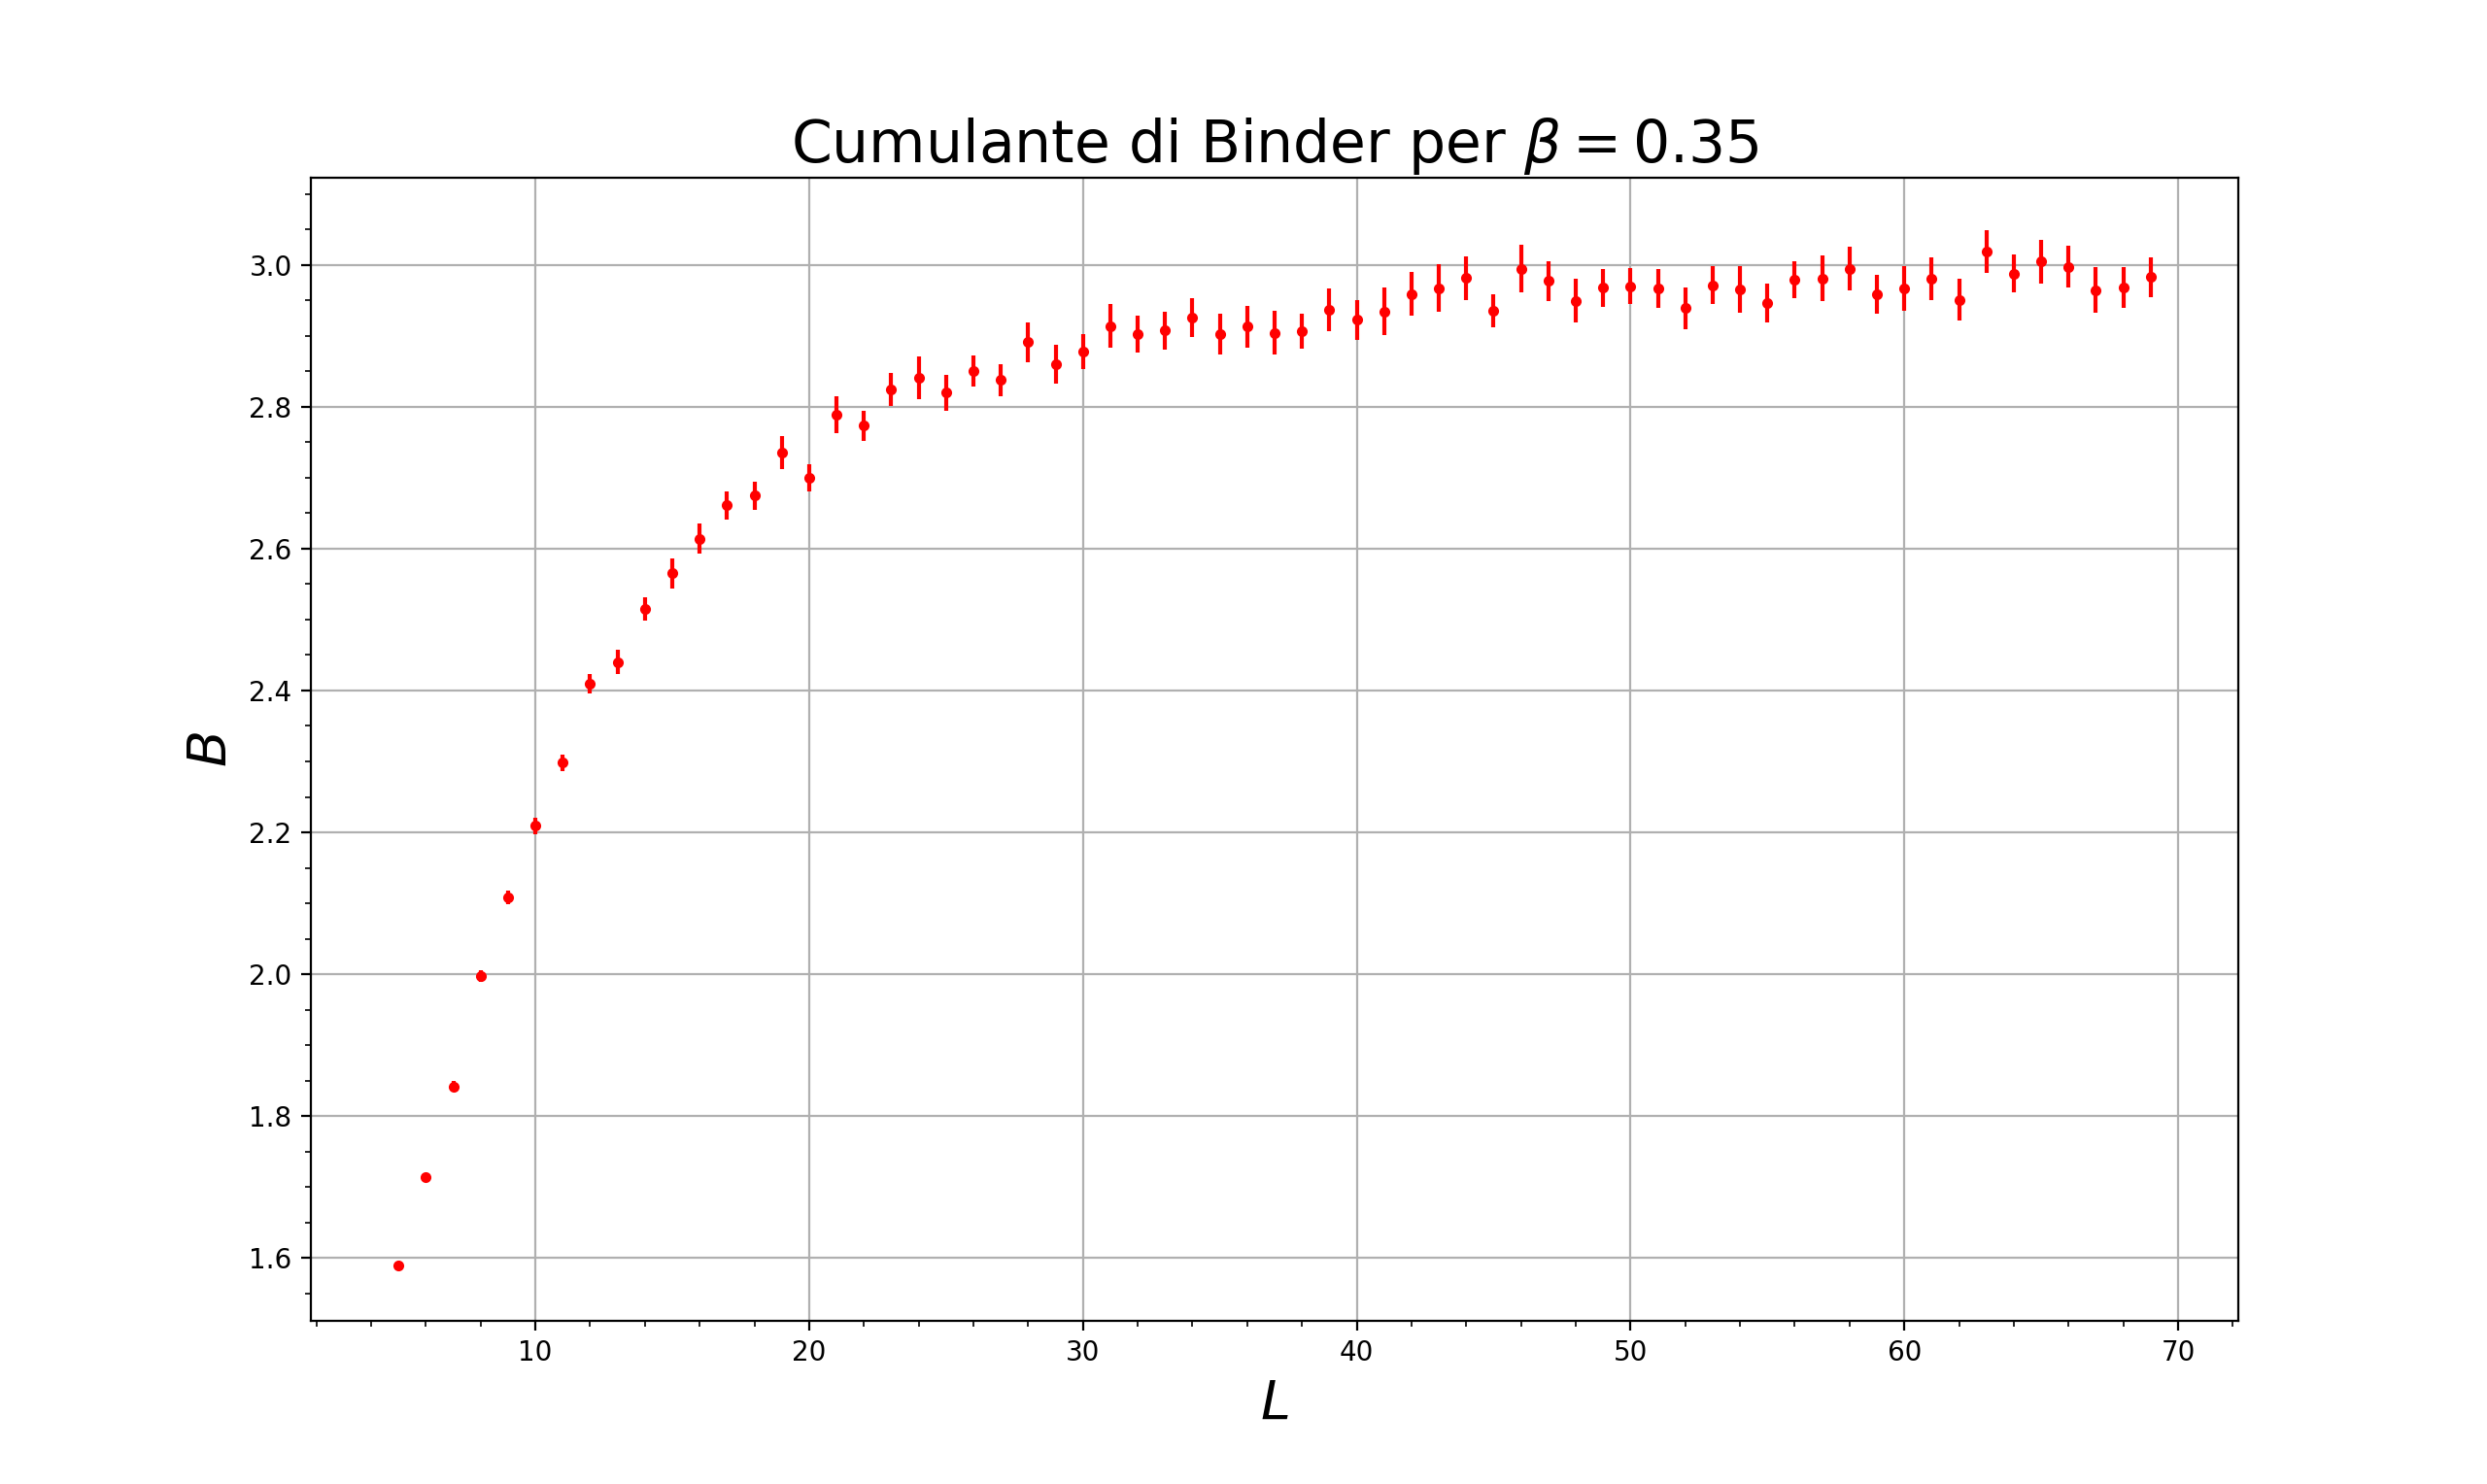
\includegraphics[width=1\linewidth]{binder035}
		\caption{Cumulante di Binder $B$ al variare di $L$ alla temperatura $\beta=0.35$.}
		\label{binder035}
	\end{figure}


	Per maggiore accuratezza, si è realizzato un fit per stimare il cumulante di Binder nel limite termodinamico $L \rightarrow \infty$ . Si può dimostrare che le correzioni a $B$ dal valore atteso sono dell'ordine dell'inverso del volume $L^{-2}$ per $L$ grande. Questo permette di stimare il cumulante di Binder per $L\rightarrow\infty$ tramite un fit con i dati in figura \ref{binder035}. E' stata scelta come funzione di fit la seguente funzione: $$f(x)\coloneqq a+bx^2$$ dove $x$ corrisponde alla variabile $L^{-1}$ e $a$ è il parametro da determinare. Infatti, deve essere $$a=\lim_{L \to \infty}B\text{ .}$$
	 Usando i valori di $B$ in corrispondenza di $L\ge16$, il risultato del fit è: $$\lim_{L \to \infty}B=3.003 \pm 0.004 $$ con un chi quadro ridotto di $\chi^2/NDF=0.51$. Il risultato $B=3.003 \pm 0.004 $ è in accordo con il valore atteso del cumulante di Binder sopra la temperatura critica.
	\item \emph{Caso} $\beta=0.45$ :\\
	Dalla figura \ref{binder045} (che si riferisce al caso $\beta=0.45$) si osserva che $B$ tende a $1$ per $L$ sufficientemente grande, il che rispetta le aspettative per una temperatura minore della temperatura critica (equazione \ref{BinderTc}).
	\begin{figure}[h!]%vedere programma binder.c
		\centering
		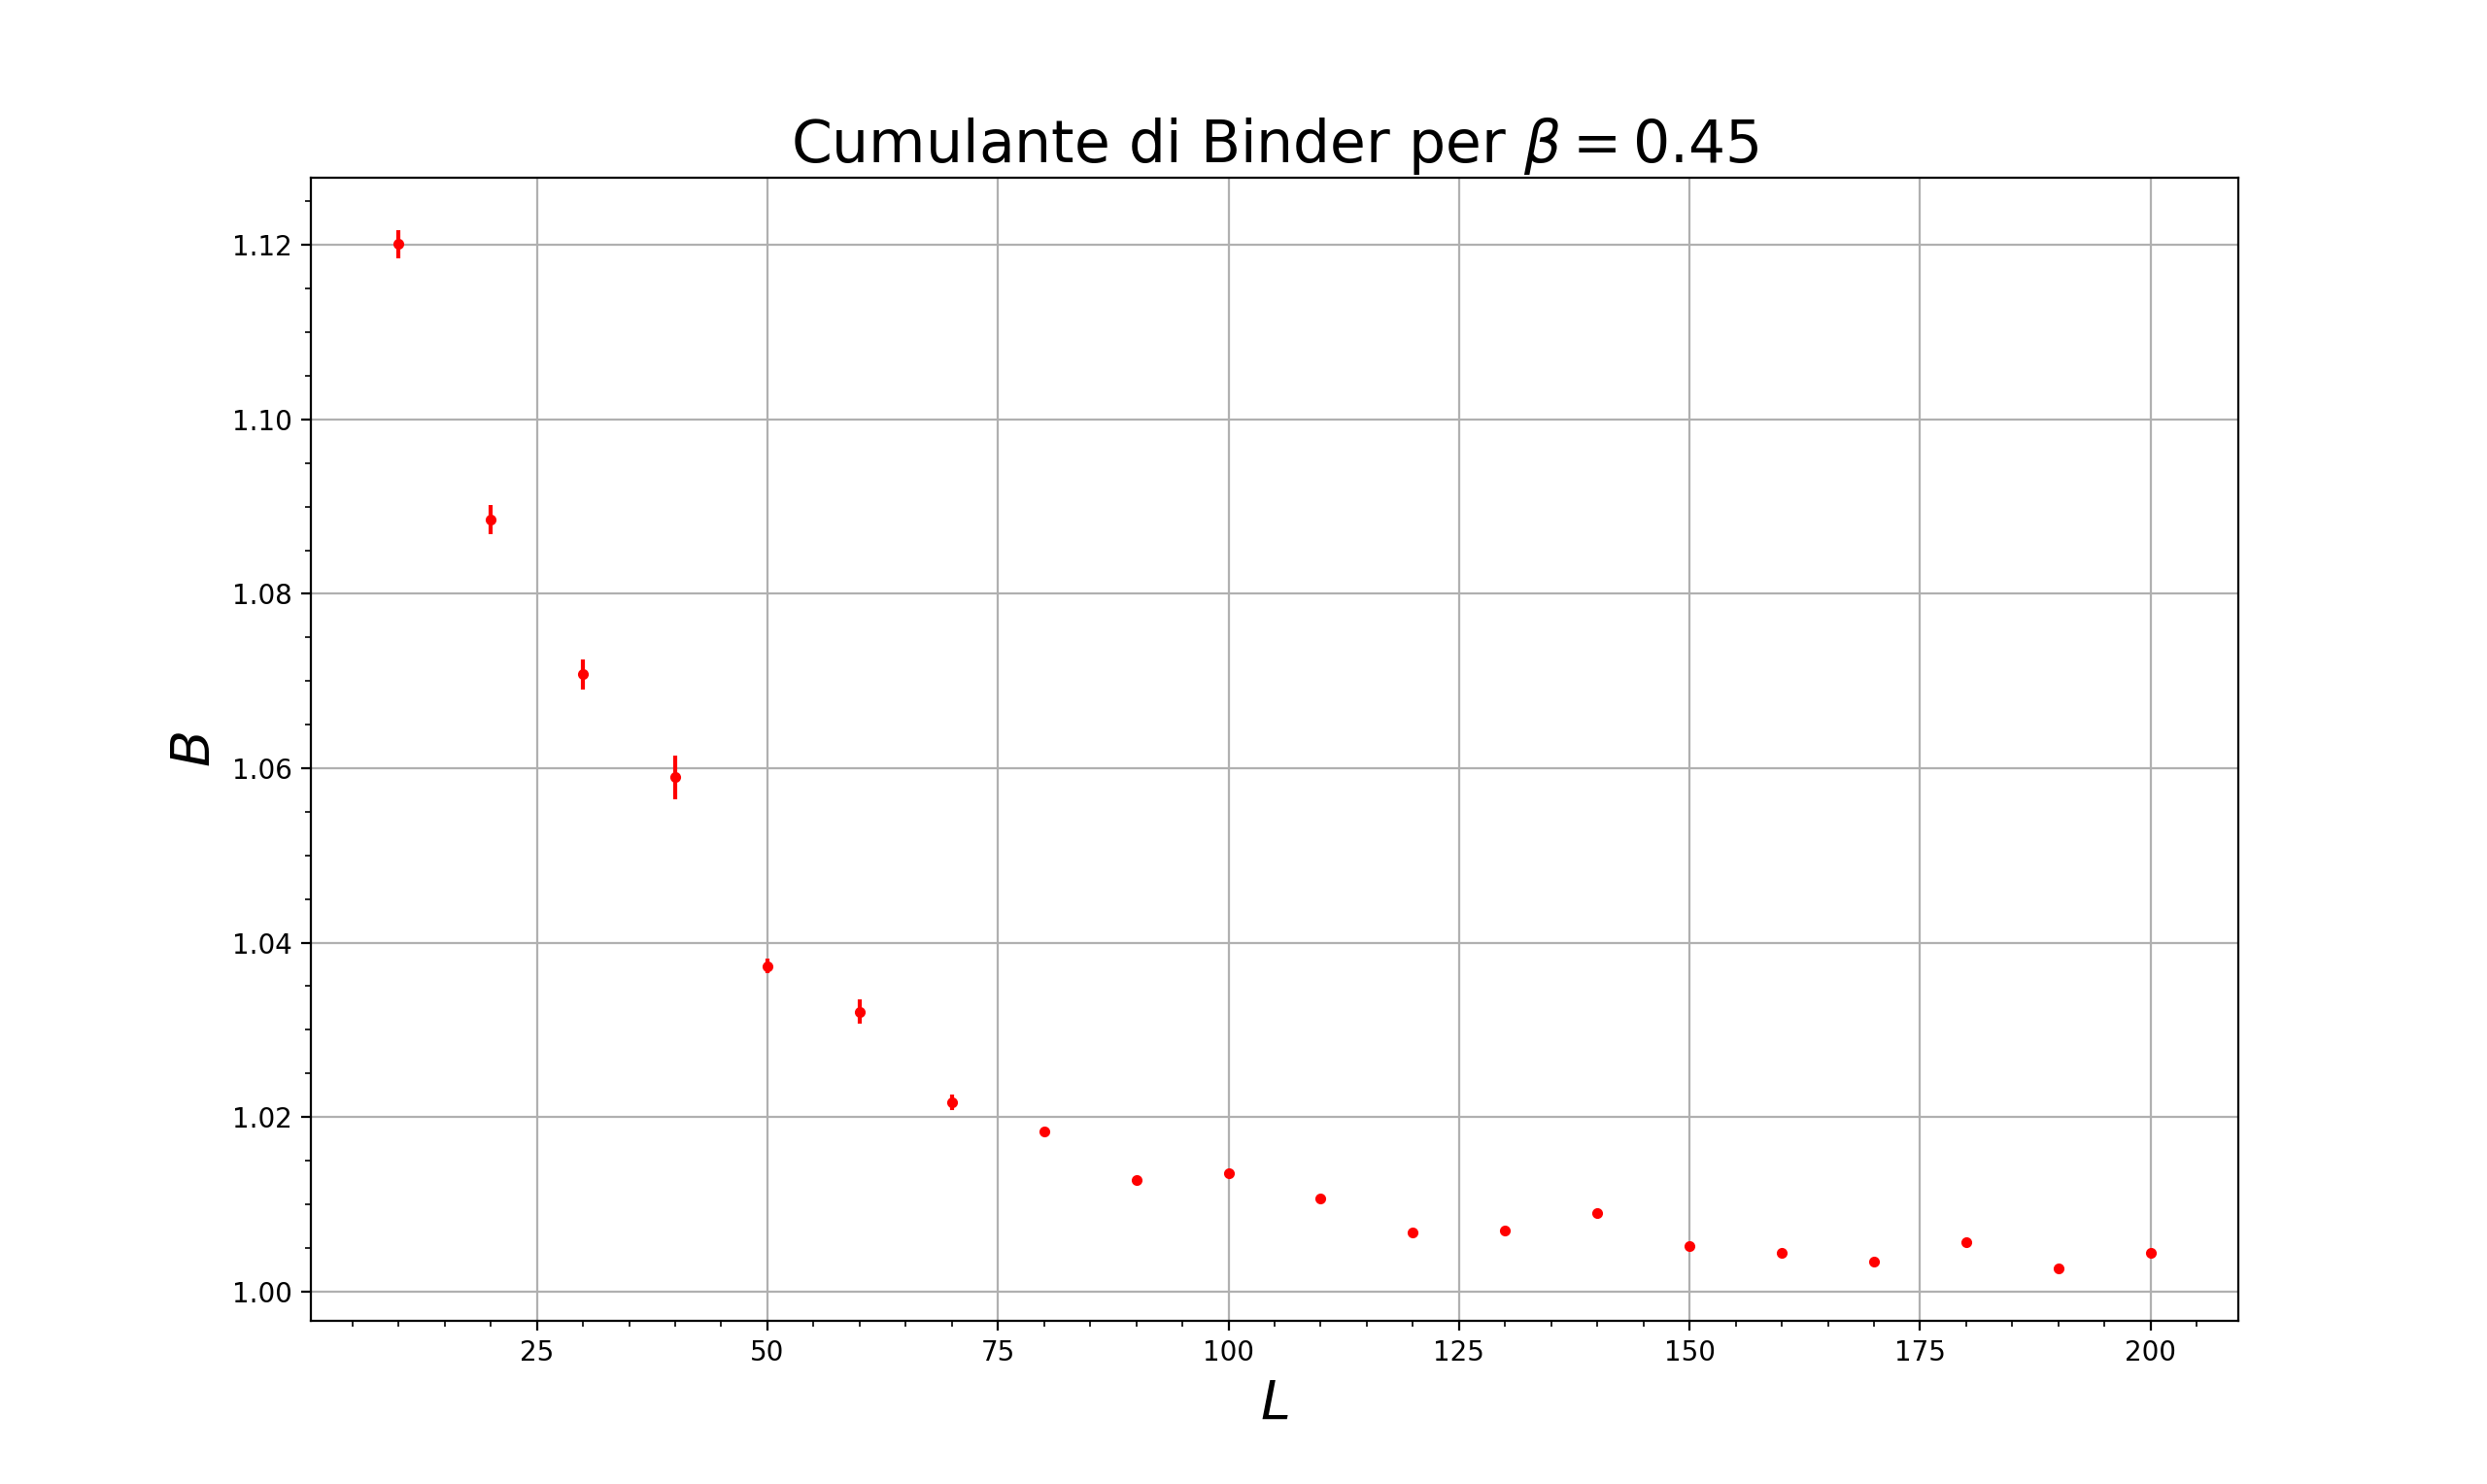
\includegraphics[width=1\linewidth]{binder045}
		\caption{Cumulante di Binder $B$ al variare di $L$ alla temperatura $\beta=0.45$.}
		\label{binder045}
	\end{figure}
\end{itemize}

	Ne concludiamo, dunque, che $\beta=0.35$ corrisponde alla fase non rotta, mentre $\beta=0.45$ corrisponde alla fase rotta.
	\subsubsection{Commento sul cumulante di Binder a temperatura $\beta=0.45$}
	L'andamento atteso del cumulante di Binder per $\beta=0.45$ per $L$ sufficientemente grande è $B\sim1+1/L^2$, cioè $B$ deve essere monotono decrescente per $L$ grande. Ciò è in contrasto con l'andamento oscillante entro l'incertezza che si osserva in figura \ref{binder045}. Ne deduciamo che l'errore è sottostimato. Il motivo di questa sottostima dell'errore risiede nel fatto che le misure diventano sempre più correlate quanto più la temperatura è vicina alla temperatura critica e quanto più $L$ è grande. A temperatura $\beta=0.45$ per reticoli grandi, l'algoritmo non riesce a campionare il tunneling tra configurazioni con magnetizzazione di segno opposto ma campiona solo configurazioni con segno costante della magnetizzazione (ad esempio come si osserva in figura \ref{fig:magnstepbeta035} per $L=50$). Per risolvere questo problema, bisognerebbe prendere un numero molto maggiore di misure. 

	
	
\subsubsection{Cumulante di Binder per temperatura $\beta=0.50$}
In figura \ref{binder050} viene riportato il cumulante di Binder al variare di $L$ per $\beta=0.50$, che corrisponde ad una temperatura sia minore della temperatura critica sia sufficientemente lontana da essa (al fine di evitare i problemi di sottostima dell'errore riscontrati con $\beta=0.45$). Ogni valore di $B$ in figura \ref{binder050} è stato ottenuto a partire da $30000$ misure di magnetizzazione e ognuna di esse è stata presa ogni 50 chiamate della subroutine update\_metropolis.
	\begin{figure}[h!]%vedere programma binder.c
	\centering
	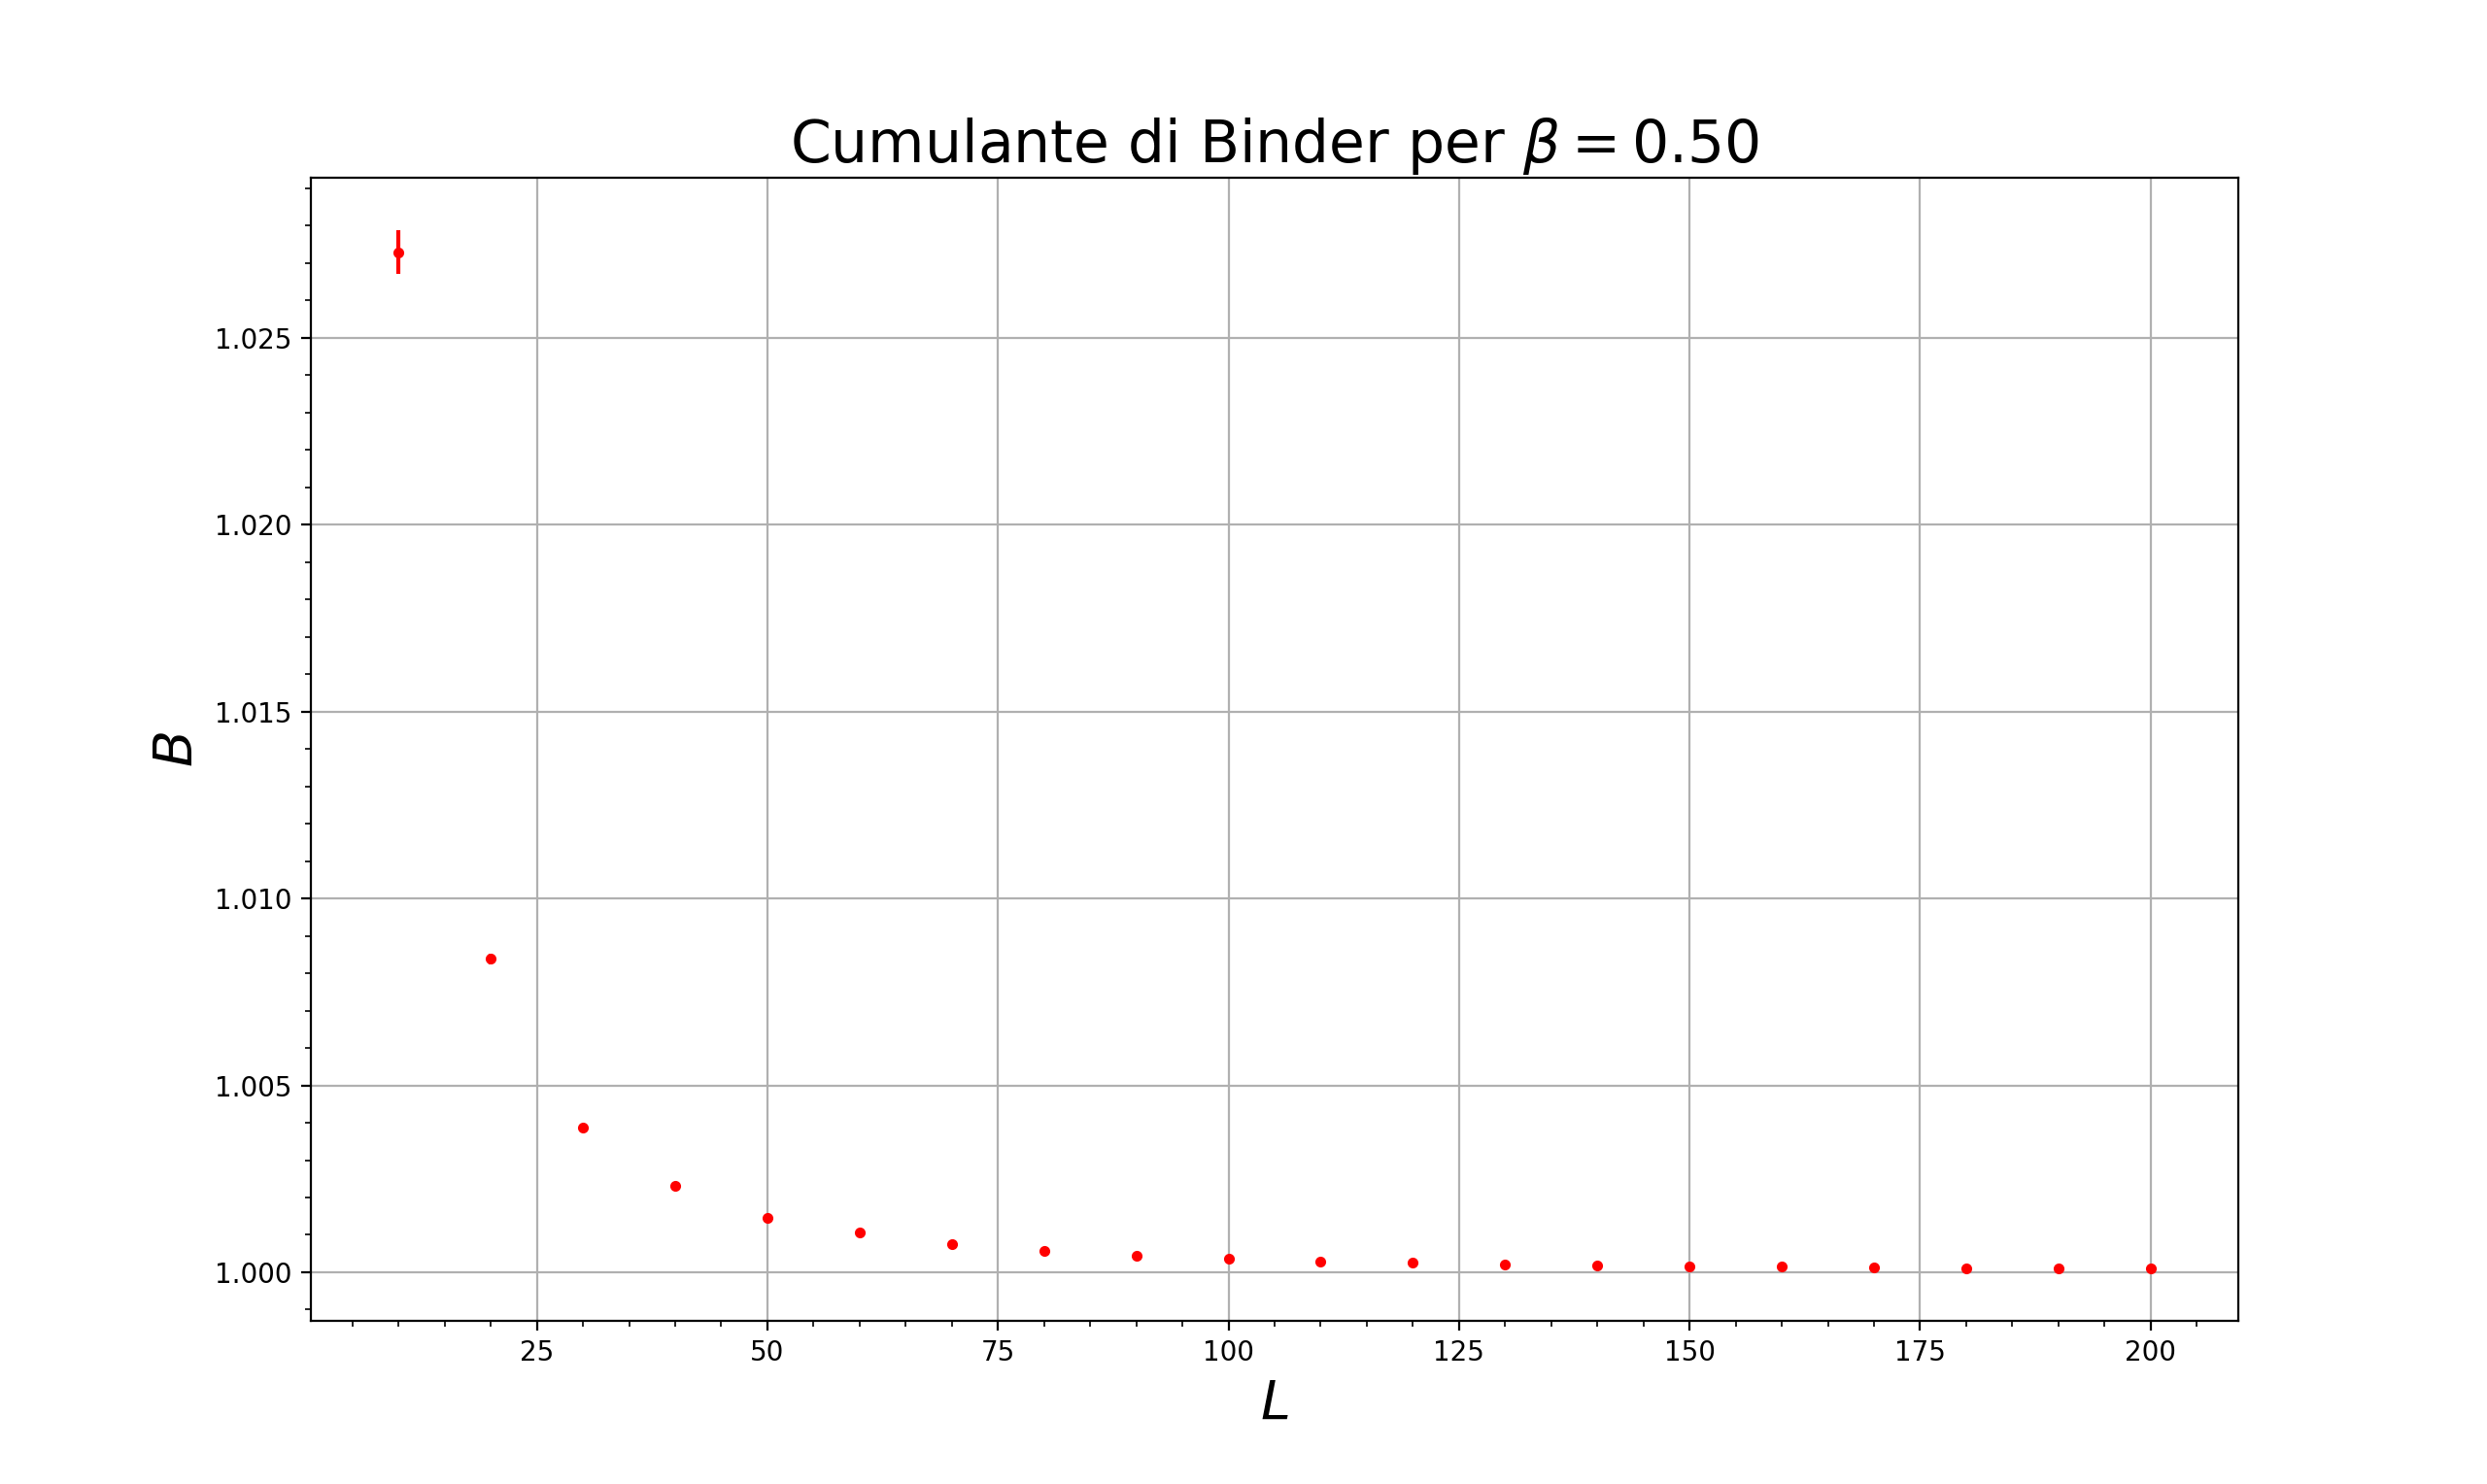
\includegraphics[width=1\linewidth]{binder050}
	\caption{Cumulante di Binder $B$ al variare di $L$ alla temperatura $\beta=0.50$.}
	\label{binder050}
\end{figure}


In figura \ref{binder050} non si osserva l'inatteso andamento oscillante riscontrato in figura \ref{binder045}, ma si osserva un andamento monotono decrescente in accordo con le previsioni teoriche (che prevedono che $B$ si avvicina ad $1$ con una correzione proporzionale a $1/L^2$). Anche in questo caso si è realizzato un fit (con funzione di fit $f(x)\coloneqq a+bx^2$ dove $x=L^{-1}$) per stimare il cumulante di Binder nel limite termodinamico $L \rightarrow \infty$. Usando i valori di $B$ per $L\ge140$ in figura  \ref{binder050}, la stima è: 
$$\lim_{L \to \infty}B=1.000000\pm0.000001$$ con un chi quadro ridotto di $\chi^2/NDF=0.31$. Il risultato è in accordo con il valore atteso del cumulante di Binder sotto la temperatura critica.

\subsubsection{Bootstrap, bootstrap con binning e stima dell'errore sul cumulante di Binder}\label{ParErrBinder}
Il cumulante di Binder è stato calcolato a partire dalle misure della magnetizzazione ottenute usando l'algoritmo Metropolis. Dato che quest'ultimo (essendo un \emph{metodo Monte-Carlo} basato su \emph{Catena di Markov}) genera misure autocorrelate e dato che il cumulante di Binder $B$ è un funzionale non banale della distribuzione di probabilità\footnote{Per "funzionale non banale della distribuzione di probabilità" si intende un funzionale che non sia semplicemente un valor medio sulla distribuzione di probabilità di una funzione della variabile stocastica.}, l'errore su $B$ è stato stimato adottando il metodo \emph{bootstrap con binning}.

Il \emph{bootstrap} (senza binning) è una tecnica statistica di ricampionamento che permette di ottenere una buona stima dell'errore statistico, supponendo che i dati siano statisticamente indipendenti. L'idea è estrarre, dal campione originale di $N$ dati, $M$ nuovi campioni \emph{fake} formati da $N$ dati selezionati in modo random dal campione originale. Successivamente, si calcola la quantità di interesse\footnote{Nel caso in esame, la quantità di interesse è il cumulante di Binder.} $B_i$ a partire dall'$i$-esimo campione fake per ogni $i=1\text{, 2, ... , }M$.  La stima dell'errore è ottenuta dalla deviazione standard di $\{B_i\}$:
$$\text{Errore su } B\simeq \sqrt{\frac{1}{M}\sum_{i=1}^{M}B_i^2-\left(\sum_{i=1}^{M}B_i\right)^2}$$

Il \emph{bootstrap con binning} è una generalizzazione della tecnica precedente al caso in cui i dati siano autocorrelati. Sia $Q$ un numero naturale molto minore del numero di dati del campione originale. Ogni campione fake è costruito nel seguente modo: si estrae un dato in modo random dal campione originale, i $Q$ dati consecutivi ad esso si inseriscono nel campione fake, si ripete questa procedura $N/Q$ volte. Analogamente al caso precedente, si calcolano le quantità di interesse $B_i$ e successivamente si ricava la deviazione standard (che dipende da $Q$). La stima corretta dell'errore è data dal valore dell'asintoto orizzontale della deviazione standard (vista come funzione di $Q$).\footnote{In questa spiegazione semplificativa del \emph{boostrap con binning} sono state omesse alcune sottigliezze tecniche che sono state adottate in questo elaborato. Ad esempio: \begin{itemize}
\item $Q$ non è scelto necessariamente tra i divisori di $N$;
\item Se il dato selezionato in modo random dal campione originale ha un numero di dati consecutivi minore di $Q$ (questa condizione si verifica se il dato è "verso la fine" del campione originale), allora nel campione fake si inseriscono i dati compresi da quello selezionato all'ultimo dato del campione originale.
\end{itemize}
Questi due punti implicano che il numero di dati in ognuno dei campioni fake può essere non esattamente $N$.} In figura \ref{func_boot} è riportato il nostro codice che implementa il bootstrap con binning.
	\begin{figure}[h!]%vedere programma binder.c
	\centering
	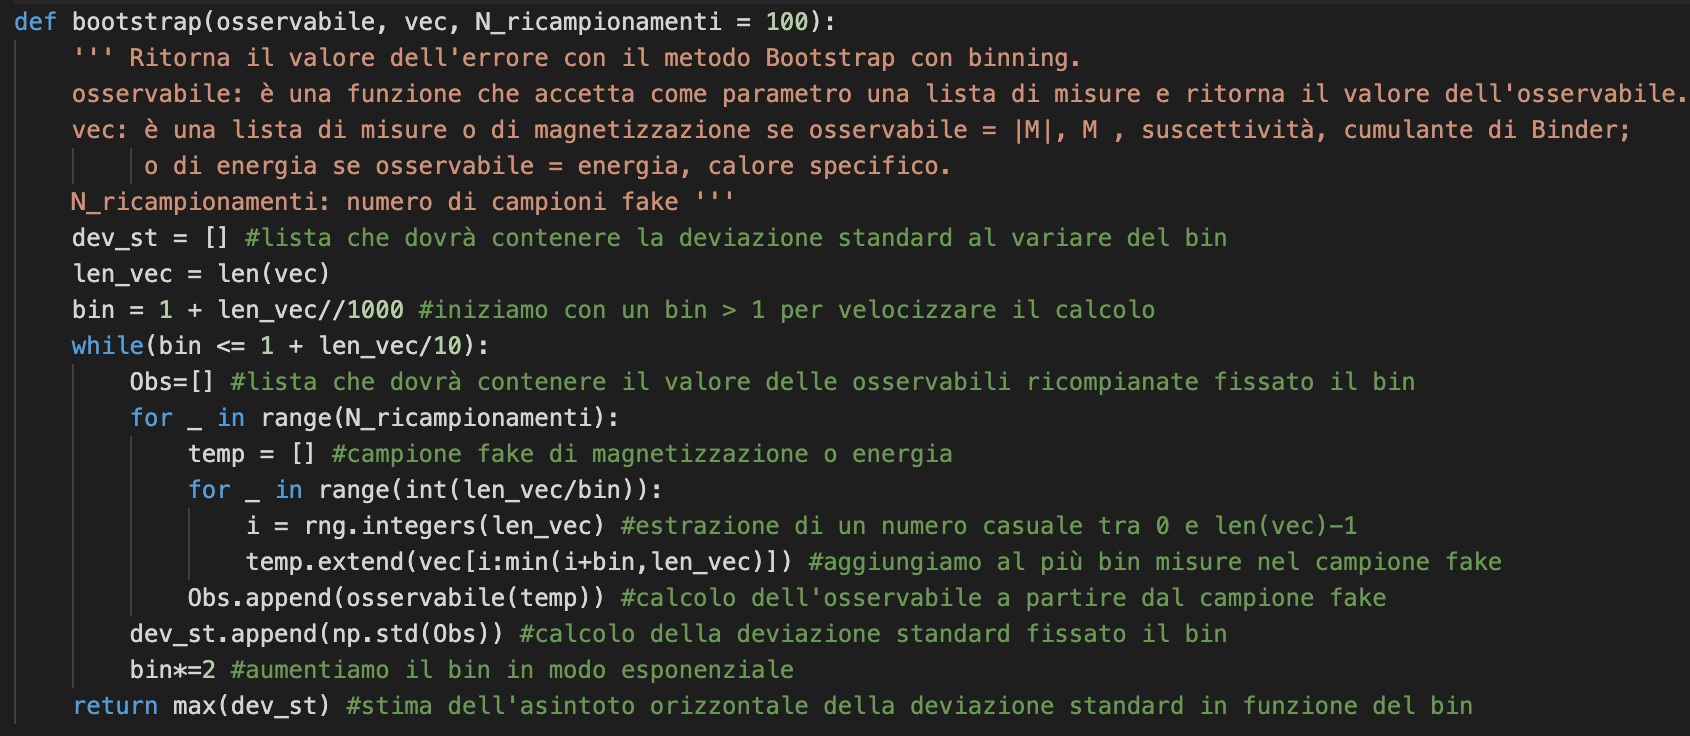
\includegraphics[width=1\linewidth]{func_boot}
	\caption{Funzione scritta in Python3 che ritorna il valore dell'errore calcolato con il bootstrap con binning. La funzione \emph{bootstrap} accetta come parametri la funzione \emph{osservabile}, la lista di misure (estratta dalle storie montecarlo ricavate con un programma in C) e il numero di campioni fake. L'asintoto orizzontale è stimato prendendo il massimo delle deviazioni standard al variare della lunghezza del bin.}
	\label{func_boot}
\end{figure}


\newpage
\section{Esponenti critici}
%forse questa roba va messa nella teoria??
Si vuole studiare il modello in analisi intorno alla transizione di fase ferromagnetica. Il comportamento intorno alla temperatura critica si può analizzare per mezzo degli \emph{esponenti critici}, che verranno definiti nei paragrafi seguenti. Inoltre, si userà $V\coloneqq L^2$ per indicare il volume e $t$ per indicare la \emph{temperatura ridotta} $$t \coloneqq\frac{T-T_c}{T_c}\text{ .}$$
\subsection*{Magnetizzazione e esponente critico $\beta$}
Nella trattazione si userà la magnetizzazione $$M\coloneqq\frac{1}{V}\sum_{i}s_i\text{ .}$$ L'andamento atteso è $M \sim |t|^{\beta}$ in un intorno destro di $t=0$ e $M\sim 0$ in un intorno sinistro. 

\subsection*{Lunghezza di correlazione e esponente critico $\nu$}
Un'altra quantità che caratterizza il comportamento critico è la  la \emph{lunghezza di correlazione} $\xi$. Essa è definita a partire dall'andamento della \emph{funzione a due punti connessa} $\langle s_is_j\rangle_c$ :
\begin{center}
$\langle s_is_j\rangle_c \coloneqq \langle s_is_j\rangle-\langle s_i\rangle\langle s_j\rangle\approx e^{-\frac{|i-j|}{\xi}}\quad$ per $|i-j|\rightarrow\infty$
\end{center}
Ad una data temperatura $T>T_c$, intuitivamente $\xi$ rappresenta la dimensione del più grande dominio di spin orientati allo stesso modo. Per $T\rightarrow T_c$ si formano dei domini che comprendono porzioni di lati opposti del reticolo (come è suggerito dalla figura \ref{reticoli}).\\ Quindi se il reticolo è infinitamente esteso, si ha: 
$$\lim_{T\to T_c}\xi=\infty$$
Più precisamente, l'andamento intorno al valore critico è:
\begin{equation}\label{eq:lunghezzadicor}
	\xi \sim |t|^{-\nu}
\end{equation}
dove l'esponente critico $\nu>0$ è lo stesso sia per $t\rightarrow 0^+$ che per $t\rightarrow 0^-$. Questa proprietà è vera anche anche per gli esponenti critici successivamente citati.

\subsection*{Suscettività e esponente critico $\gamma$}
La \emph{suscettività magnetica} $\chi$ si definisce come:
\begin{equation}\label{eq:suscettivita}
	\chi \coloneqq\frac{\partial \langle M \rangle}{\partial h} 
\end{equation}
L'osservazione fondamentale è che $\chi$ si può scrivere in termi della varianza di $M$:
\begin{equation}\label{eq:fluttuazionesuscettivita}
\chi= \beta V[\langle M ^2 \rangle - \langle M\rangle^2] 
\end{equation}
Ciò è utile perché, dal punto di vista numerico, è più facile calcolare una varianza rispetto ad una derivata.\\
Nel caso di reticolo infinito, l'andamento critico atteso è $\chi \sim |t|^{-\gamma}$.

\subsection*{Calore specifico  e esponente critico $\alpha$}
Il \emph{calore specifico} $C$ si definisce come la derivata rispetto alla temperatura della densità di energia media per sito. Esso si può scrivere in termini della varianza dell'energia media per sito $\epsilon$:
\begin{equation}
C \coloneqq \frac{\partial \langle \epsilon \rangle}{\partial T} \propto V [\langle \epsilon ^2 \rangle - \langle \epsilon \rangle^2] 
\label{eq:calorespecifico}
\end{equation}
dove, nel caso di campo magnetico nullo $h=0$, si ha
\begin{equation}
\epsilon=-\frac{1}{V}\sum_{\langle i,j\rangle}s_i s_j
\label{enpersito}
\end{equation}
Nel caso di reticolo infinito, l'andamento critico atteso è $C\sim |t|^{-\alpha}$.
 \subsection{Valori teorici degli esponenti critici}
Gli esponenti critici del modello ising 2D si possono calcolare analitamente e si trova:
\begin{equation*}
\nu =1  \qquad \beta =1/8 \qquad \gamma = 7/4  \qquad \alpha = 0 
\end{equation*}
Questo è il quadro teorico che verrà verificato numericamente in questo elaborato.


\section{Campionamento}\label{Campionamento}
Dato che tutte le osservabili di interesse (suscettività, valore assoluto della magnetizzazione, calore specifico, cumulante di binder e energia per sito) sono funzionali di valor medi di potenze di energia o magnetizzazione, abbiamo campionato le storie montecarlo di energia e magnetizzazione per ogni valore di $L$ e $\beta$ desiderato e successivamente abbiamo calcolato le osservabili. I valori di $L$ considerati sono da $10$ a $50$ a step di $5$. 



Per $L = 10$ sono state campionate storie montecarlo per $\beta\in[0.001,1.000]$ a step di $\delta \beta=0.001$ (ciò perché nel paragrafo \ref{CompAsint} vogliamo analizzare il comportamento ad alte temperature e a basse temperature). Ogni storia contiene $10000$ misure ed ognuna di esse è presa ogni $10$ chiamate della subroutine \emph{update\_metropolis}. 


Per $L\ne 10$, i valori di $\beta$ considerati sono $\beta\in[0.3400,0.4800]$ a step di $\delta \beta=0.0005$ nell'intervallo $[0.4000,0.4500]$ (ciò perché ci interessa il comportamento attorno alla temperatura critica) mentre a step di $\delta \beta=0.0010$ all'infuori di tale intervallo. Ogni storia contiene $10000$ misure ed ognuna di esse è presa ogni $100$ chiamate della subroutine \emph{update\_metropolis}. 



Fissato $L$, al fine di ridurre il tempo di termalizzazione per la simulazione ad una temperatura $\beta$, è stata assegnata come configurazione iniziale del reticolo la configurazione finale associata alla simulazione del $\beta$ precedente (questa osservazione riduce significativamente il tempo di termalizzazione in quanto i valori campionati di $\beta$ sono vicini tra di loro). Inoltre come configurazione iniziale del primo valore di $\beta$ considerato (dato che questo si trova ad una temperatura $T$ sopra quella critica) è stata adottata una configurazione in cui tutti gli spin sono random.

Gli errori sulle osservabili sono stati calcolati con il metodo \emph{bootstrap con binning} (introdotto nel paragrafo \ref{ParErrBinder}).
 
Il motivo per cui all'incirca nell'intervallo $\beta\in[0.43,0.45]$ osserviamo che gli errori sulle osservabili aumentano (come si può osservare ad esempio dal plot della suscettività in figura \ref{suscettivitabeta}) risiede sia nel fatto che abbiamo preso un numero di misure costante al variare di $\beta$ e sia nel fatto che vicino alla temperatura critica le misure diventano molto correlate. Infatti, vicino la temperatura critica si formano domini macroscopici di spin orientati tutti allo stesso modo, come è suggerito dalla figura \ref{reticoli} in cui vengono riportate configurazioni di spin ottenute per alcuni valori di $\beta$. Per perdere completamente memoria di una configurazione con un dominio di spin concordi, l'algoritmo utilizzato necessita di un numero tanto più grande di passi della catena di Markov quanto più il dominio è grande. Questo si manifesta attraverso l'aumento del tempo di autocorrelazione in corrispondenza della transizione di fase e quindi attraverso un aumento dell'errore. 
\begin{figure}[h!]%rifare nel caso
	\centering
	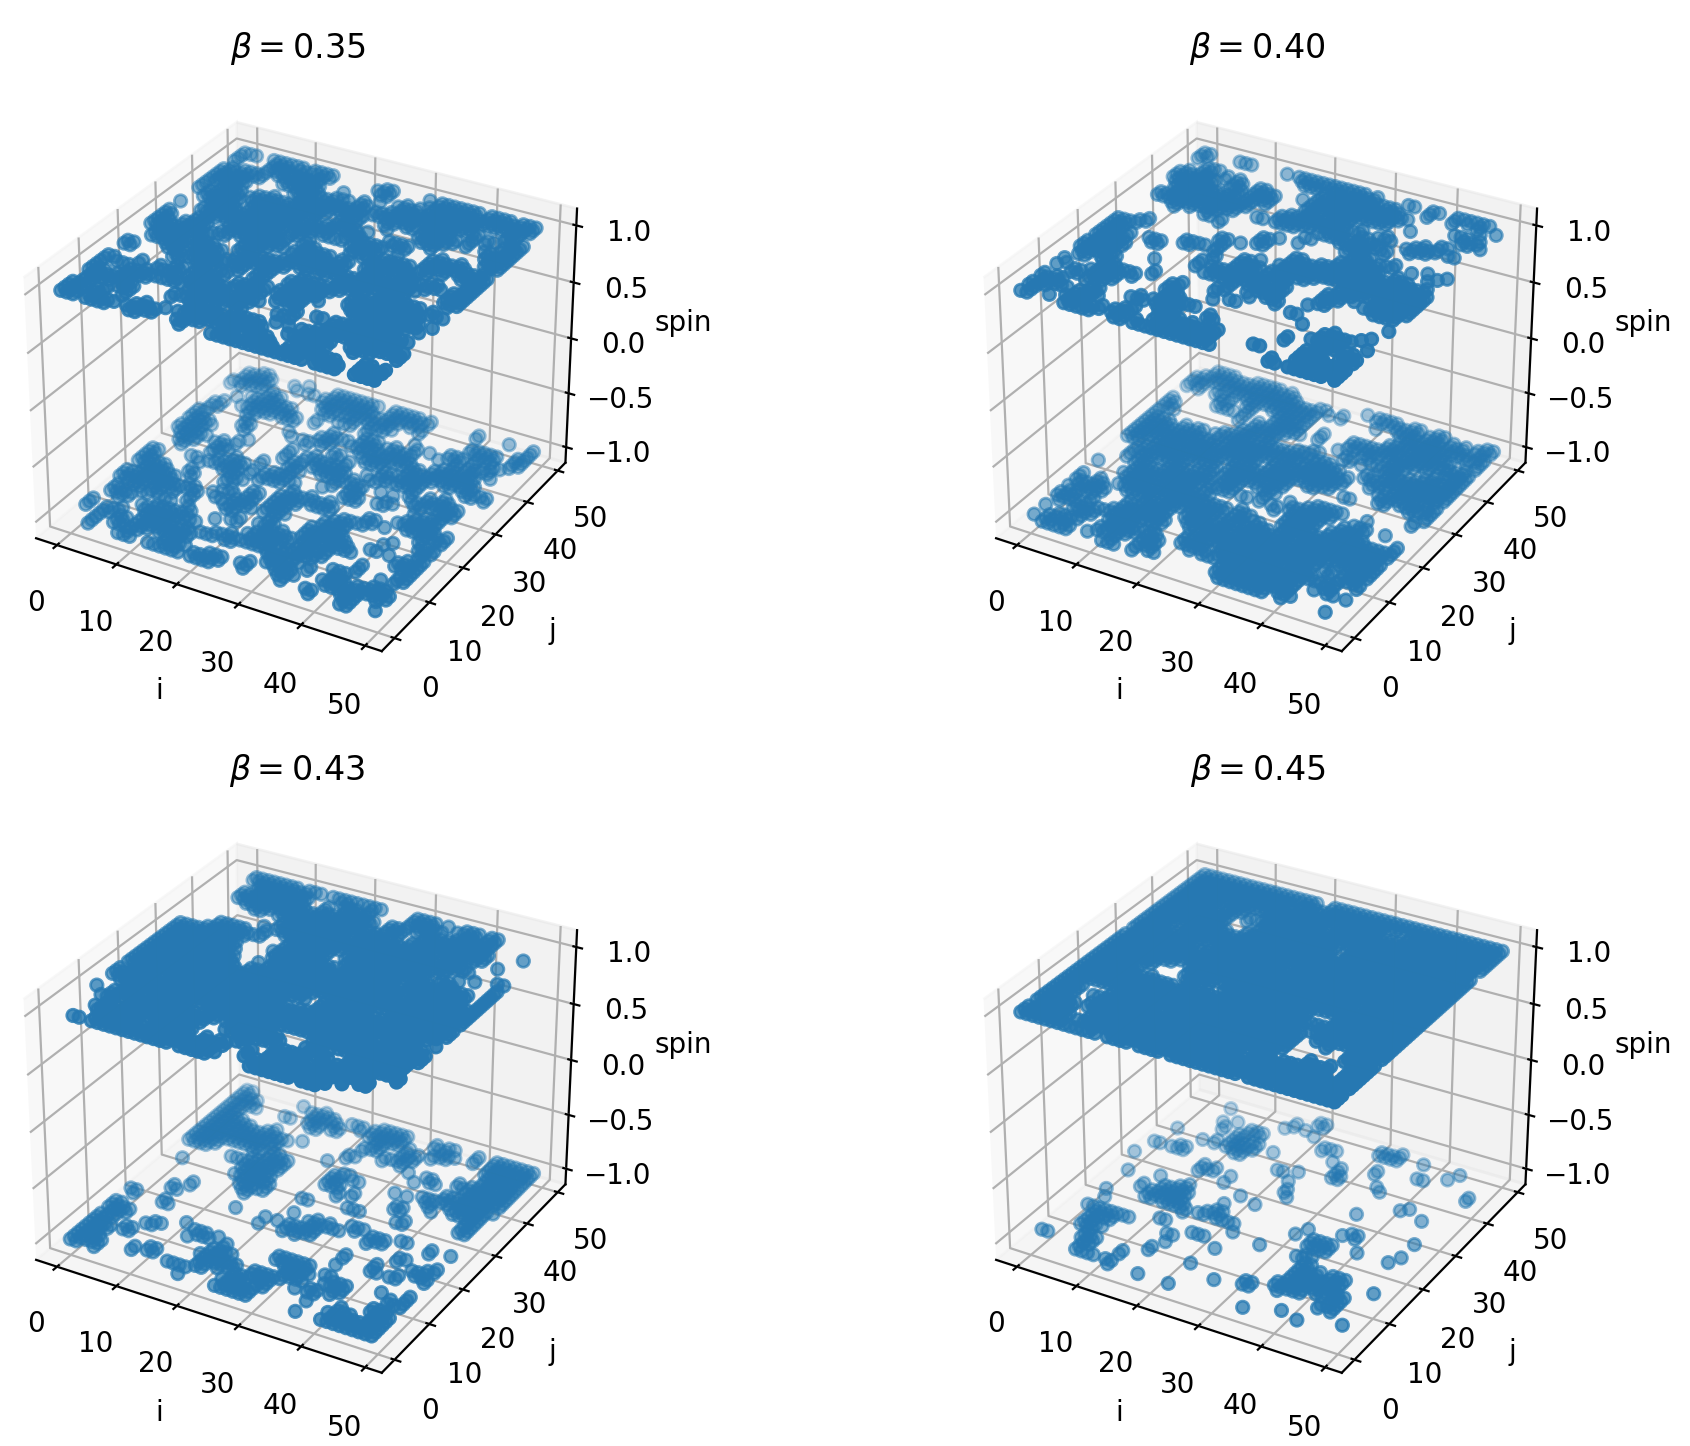
\includegraphics[width=0.7\linewidth]{reticoli}
	\caption{Configurazioni di spin del reticolo quadrato con lato $L=50$ a temperatura $\beta=$ 0.35, 0.40, 0.43 e 0.45, ottenute usando l'algoritmo Metropolis. }
	\label{reticoli}
\end{figure}



\section{Strategia numerica per la stima di $\nu$, $\gamma$ e $\beta_c$} 
Dato che nelle simulazioni numeriche il reticolo è finito la lunghezza di correlazione $\xi$ non diverge\footnote{Nel caso di $L$ finito, la funzione di partizione è una somma finita e quindi non può comparire un comportamento non analitico.}, ma ha un massimo dell'ordine di $L$ intorno alla temperatura critica:
\begin{equation}\label{ximax}
\xi_{max}\sim L
\end{equation}

L'obiettivo è studiare l'andamento critico (che si manifesta per $L\rightarrow\infty$), pur avendo a disposizione un reticolo finito (che non presenta un comportamento critico). Questa tecnica è detta \emph{finite size scaling}. In questo paragrafo stimeremo numericamente le quantità $\nu$, $\gamma$ e $\beta_c$.

Ricavando $t$ in funzione di $\xi$ dall'equazione \ref{eq:lunghezzadicor} e usando le relazioni precedenti, si ottiene:
\begin{equation}\label{espxi}
\langle |M| \rangle\sim \xi^{-\frac{\beta}{\nu}}  \qquad \qquad \chi\sim \xi^{\frac{\gamma}{\nu}}  \qquad \qquad C\sim \xi^{\frac{\alpha}{\nu}}
\end{equation}
Dato che $\xi$ non diverge, anche queste quantità non divergono e raggiungono il loro valore massimo quando $\xi$ raggiunge il suo valore massimo. In particolare, dalle equazioni \ref{ximax} e \ref{espxi} segue che:
\begin{equation*}
 \chi_{max}\sim L^{\frac{\gamma}{\nu}}  
\end{equation*}
Il primo passo della strategia è, dunque, plottare $\chi_{max}$ in funzione di $L$ e fare un fit per ricavare il rapporto $\frac{\gamma}{\nu}$.
\subsection*{Grafico della suscettività}\label{ds}
La suscettività è stata calcolata mediante la seguente formula:
\begin{equation*}
\chi\propto V[\langle M ^2 \rangle - \langle |M|\rangle^2] 
\end{equation*}
Notare che l'espressione precedente non è esattamente la varianza della magnetizzazione, per via del termine $\langle |M|\rangle^2$. Il motivo della presenza del valore assoluto è spiegato di seguito. L'obiettivo dell'analisi numerica è simulare l'andamento critico, che emerge solo per reticoli infiniti. Nel caso di reticolo infinito, sotto la temperatura critica, la magnetizzazione non presenta più le variazioni di segno mostrate in figura \ref{fig:magnstepbeta045}. Al fine di eliminare l'effetto di queste variazioni di segno nel calcolo della varianza (che porterebbero ad un valor medio di $M$ nullo e ad una sovrastima della suscettività), viene utilizzato il valore assoluto della magnetizzazione.

Il grafico\footnote{In realtà, la funzione graficata in figura \ref{suscettivitabeta} è $L^2[\langle M ^2 \rangle - \langle |M|\rangle^2]$, ovvero la suscettività riscalata per un fattore $\beta$.  Il motivo di questa scelta è per seguire la convenzione adottata a lezione. } di $\chi$ in funzione di $\beta$ è riportato in figura \ref{suscettivitabeta}. 

\begin{figure}[h!]
	\centering
	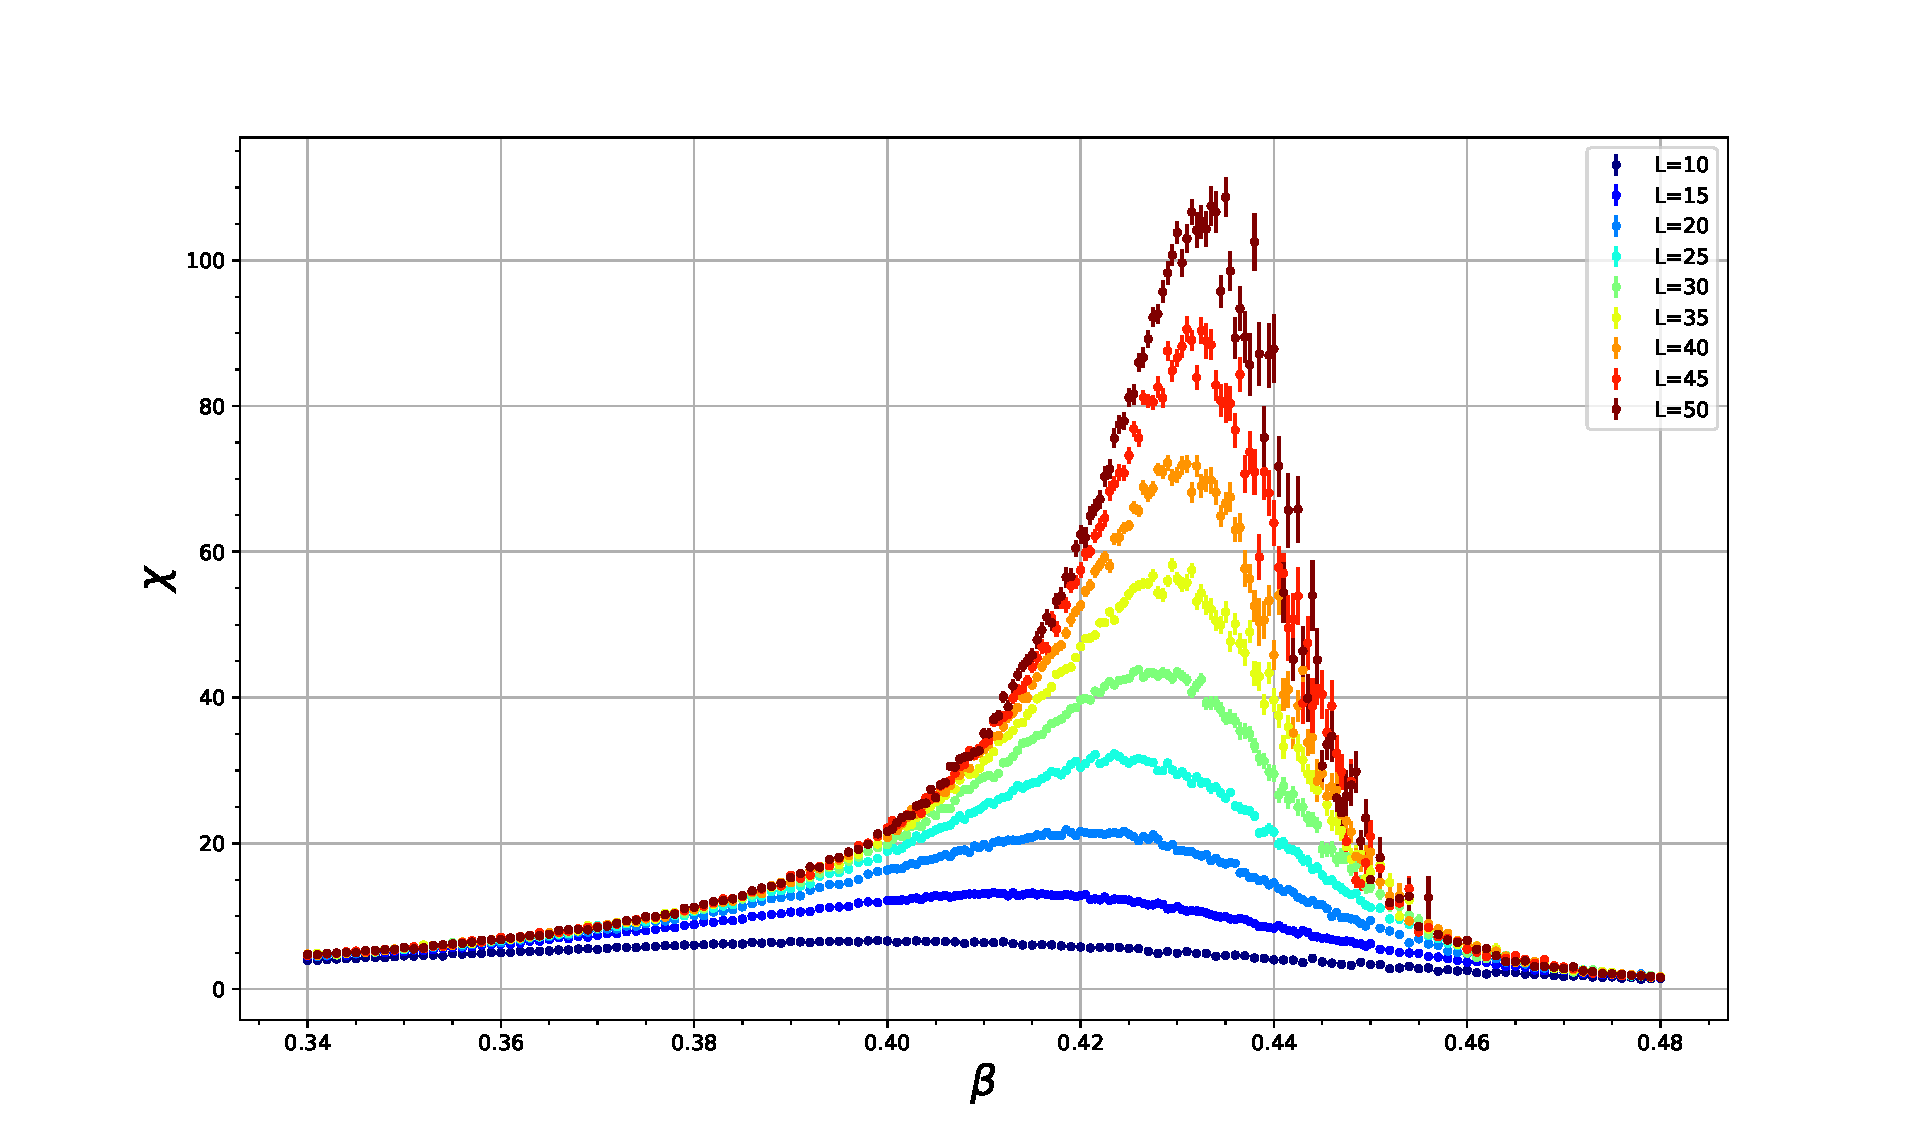
\includegraphics[width=1\linewidth]{susc_beta.pdf}
	\caption{Suscettività magnetica al variare di $\beta$ per alcuni valori di $L$.}
	\label{suscettivitabeta}
\end{figure}
Si osservi che il massimo di $\chi$ cresce all'aumentare di $L$. Ciò era atteso dato che nel limite di $L\rightarrow\infty$ la suscettività è divergente alla temperatura critica. Inoltre, i punti di massimo non sono esattamente coincidenti con la temperatura critica teorica $\beta_c\approx0.441$, ma aumentando $L$ i punti di massimo si spostano verso essa.
\subsection*{Stima dei massimi della suscettività}
Per ognuna delle 4 curve della suscettività riportate in figura \ref{suscettivitabeta}, è stato ricavato il punto di massimo $\beta_{pc}(L)$ e il massimo $\chi_{max}(L)$. Il procedimento è riportato di seguito.\\
Fissato $L$, è stato fatto un fit con la parabola $f(x)\coloneqq\chi_{max}-b(x-\beta_{pc})^2$ con i punti $(\beta,\chi)$ tali che $\beta$ appartiene ad un opportuno intervallo $[\beta_{min},\beta_{max}]$. L'intervallo, posizionato in modo che comprendeva il punto di massimo, è stato variato più volte per verificare la stabilità dei parametri da determinare, ovvero $\beta_{pc}(L)$ e $\chi_{max}(L)$. I risultati del fit sono mostrati in tabella \ref{suscmax}. %vedere cartella suscettivitàMax
%ma il chi quadro serve?!
\begin{table}[h]
\centering 
\begin{tabular}{lccr}
L & $\beta_{pc}$ & $ \chi _{max}$ & $\chi^2/ \mathrm{ndof} $\\ \hline
10 & 0.3986 $\pm$ 0.0003 & 6.57 $\pm$ 0.02 & 0.70\\
15 & 0.4128 $\pm$ 0.0004 & 13.07 $\pm$ 0.03 & 0.61\\
20 & 0.4204 $\pm$ 0.0002 & 21.49 $\pm$ 0.05 & 0.84\\
25 & 0.4240 $\pm$ 0.0001 & 31.55 $\pm$ 0.09 & 1.02\\
30 & 0.4270 $\pm$ 0.0001 & 43.27 $\pm$ 0.11 & 0.65\\
35 & 0.4287 $\pm$ 0.0002 & 56.34 $\pm$ 0.33 & 1.47\\
40 & 0.4302 $\pm$ 0.0001 & 71.49 $\pm$ 0.32 & 0.99\\
45 & 0.4314 $\pm$ 0.0002 & 88.61 $\pm$ 0.84 & 1.75\\
50 & 0.4324 $\pm$ 0.0003 & 105.44 $\pm$ 1.07 & 1.97\\
\end{tabular}
\caption{Valori ottenuti dal fit per il punto di massimo $\beta_{pc}$ e il massimo $\chi _{max}$ della suscettività $\chi$ in funzione di $\beta$ riportata in figura \ref{suscettivitabeta} per alcuni $L$.}
\label{suscmax}
\end{table}

\subsection*{Stima del rapporto $\frac{\gamma}{\nu}$}
Usando i risultati ottenuti in tabella  \ref{suscmax}, è stato fatto un fit con la funzione $f(x)\coloneqq a+bx^c$ con i punti $(L,\chi_{max})$. Il parametro $c$ corrisponde al rapporto $\gamma/\nu$, dato che l'andamento atteso è $ \chi_{max}\sim L^{\gamma/\nu}$.\\%vedere cartella GammaSuNu
Il risultato del fit è: $$\frac{\gamma}{\nu}=1.747\pm 0.005$$ che è in accordo con il valore teorico di $1.75$. Il chi quadro ridotto è di $0.44$.
\subsection*{Ipotesi di scaling e stima di $\nu$, $\gamma$ e $\beta_c$}
Per l'analisi seguente è utile introdurre e assumere l'\emph{ipotesi di scaling}: in un intorno della temperatura di transizione, dove $\xi\rightarrow\infty$, il sistema perde completamente memoria della sua struttura microscopica.\\
Utilizzando tale assunzione si può dimostrare che esiste una funzione $\phi:\mathbb{R}\rightarrow\mathbb{R}$ tale che:
\begin{equation*}
\chi(\beta,L)= L^{\frac{\gamma}{\nu}}\phi\left((\beta-\beta_c)L^{\frac{1}{\nu}}\right)
\end{equation*}
Dato che, fissato $L$, la suscettività come funzione di $\beta$ ha un massimo, anche la funzione $\phi(x)$ deve ammettere un massimo. Sia $\bar{x}$ il punto di massimo di $\phi(x)$. Al punto di massimo si ha:
\begin{equation*}
\phi(\bar{x})=\frac{\chi(\beta_{pc}(L),L)}{L^{\frac{\gamma}{\nu}}}=\phi\left((\beta_{pc}(L)-\beta_c)L^{\frac{1}{\nu}}\right)
\end{equation*}
Cioè:
\begin{equation*}
\bar{x}= \left(\beta_{pc}(L)-\beta_c\right)L^{\frac{1}{\nu}}
\end{equation*}
Dunque l'andamento del punto di massimo della suscettività al variare di $L$ è:
\begin{equation}
\beta_{pc}(L)= \beta_c+\bar{x}L^{-\frac{1}{\nu}}
\label{eq:betapc}
\end{equation}
Come atteso vale $\beta_{pc}(L)\rightarrow\beta_c$ per $L\rightarrow\infty$ (dato che $\nu>0$).\\
Facendo un fit con la funzione in equazione \ref{eq:betapc} e con i punti $(L,\beta_{pc})$ riportati in tabella \ref{suscmax}, è possibile stimare i valori di $\nu$ e $\beta_{pc}$.\\%vedere cartella FitBeta_c
I risultati del fit sono: $\beta_c=0.439\pm0.001$, $\nu=0.93\pm 0.04$ e $\bar{x}=-0.49\pm0.04$ con un chi quadro ridotto di $1.45$ . \\
E ricordando che $\frac{\gamma}{\nu}=1.747\pm 0.005$, è possibile ricavare anche una stima di $\gamma$. Si ottiene: $\gamma=1.63\pm 0.07$ .\\ Riassumendo i valori calcolati numericamente con la strategia precedente sono:\\
\begin{equation*}
\beta_c=0.439\pm0.001  \qquad \nu=0.93\pm 0.04 \qquad \gamma=1.63\pm 0.07
\end{equation*}
che sono in accordo con i valori teorici.


\subsection*{Verifica dell'ipotesi di scaling}
L'ipotesi di scaling implica l'esistenza di una funzione $\phi$ di una sola variabile tale che:
\begin{equation*}
\chi(\beta,L)L^{-\frac{7}{4}}= \phi\left((\beta-\beta_c)L\right)
\end{equation*}
dove sono stati direttamente sostituiti i valori teorici di $\nu$ e $\gamma$. 

Dunque per verificare a posteriori l'ipotesi di scaling, è sufficiente fare un plot con asse orizzontale $(\beta-\beta_c)L$, asse verticale $\chi(\beta,L)L^{-\frac{7}{4}}$ e controllare se i punti plottati si vanno a disporre su una sola curva. Usando le misure della suscettività riportate in figura \ref{suscettivitabeta}, si ottiene il grafico in figura \ref{fig:suscettivitalviararedibetaeL}. %vedere cartella IpotesiDiScalingSusc
\begin{figure}[h!]
	\centering
	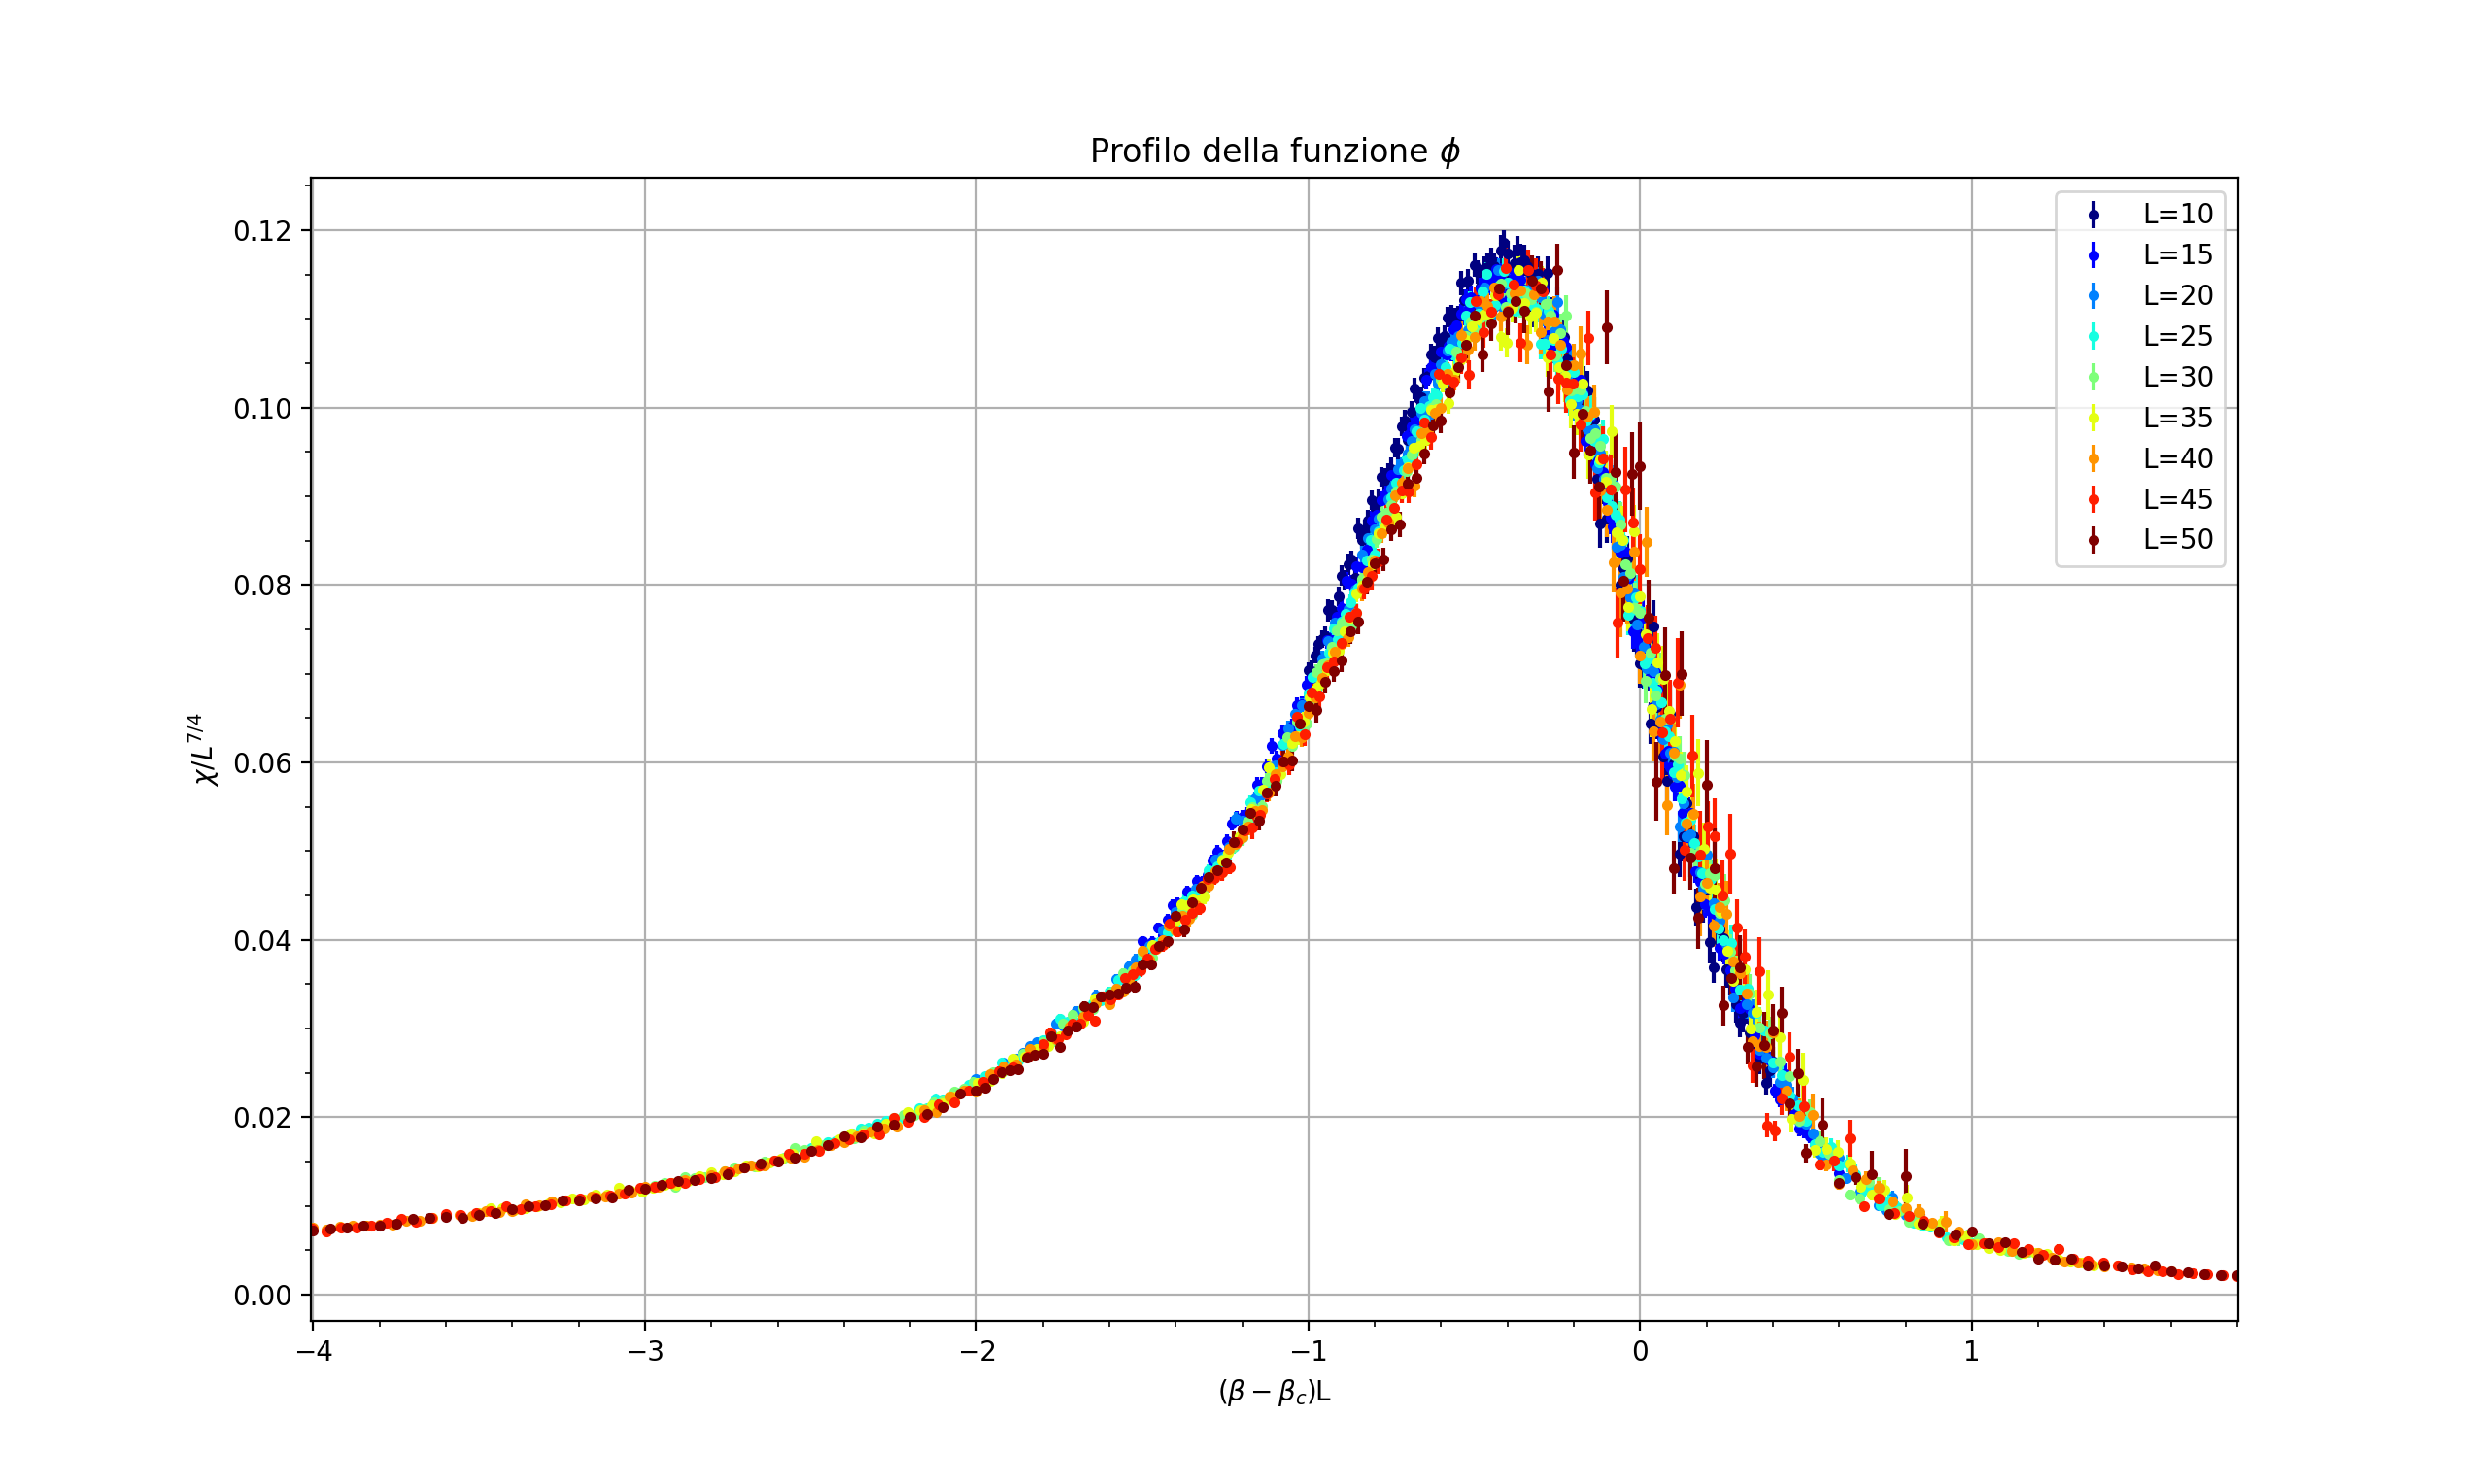
\includegraphics[width=1\linewidth]{susc_norm}
	\caption{$\chi(\beta,L)L^{-\frac{7}{4}}$ al variare della variabile di scaling $(\beta-\beta_c)L$.}
	\label{fig:suscettivitalviararedibetaeL}
\end{figure}\\
Dato che i punti collassano sulla stessa curva, si conclude che l'ipotesi di scaling è verificata.
\newpage

\section{Osservazioni sul plot di $\langle|M|\rangle$}
Il grafico del valor medio del valore assoluto della magnetizzazione $\langle |M|\rangle$ in funzione di $\beta$ è riportato in figura \ref{fig:magnass}.

\begin{figure}[h!]%vedere magn_ass.c e cartella AbsMagnetizzazione
	\centering
	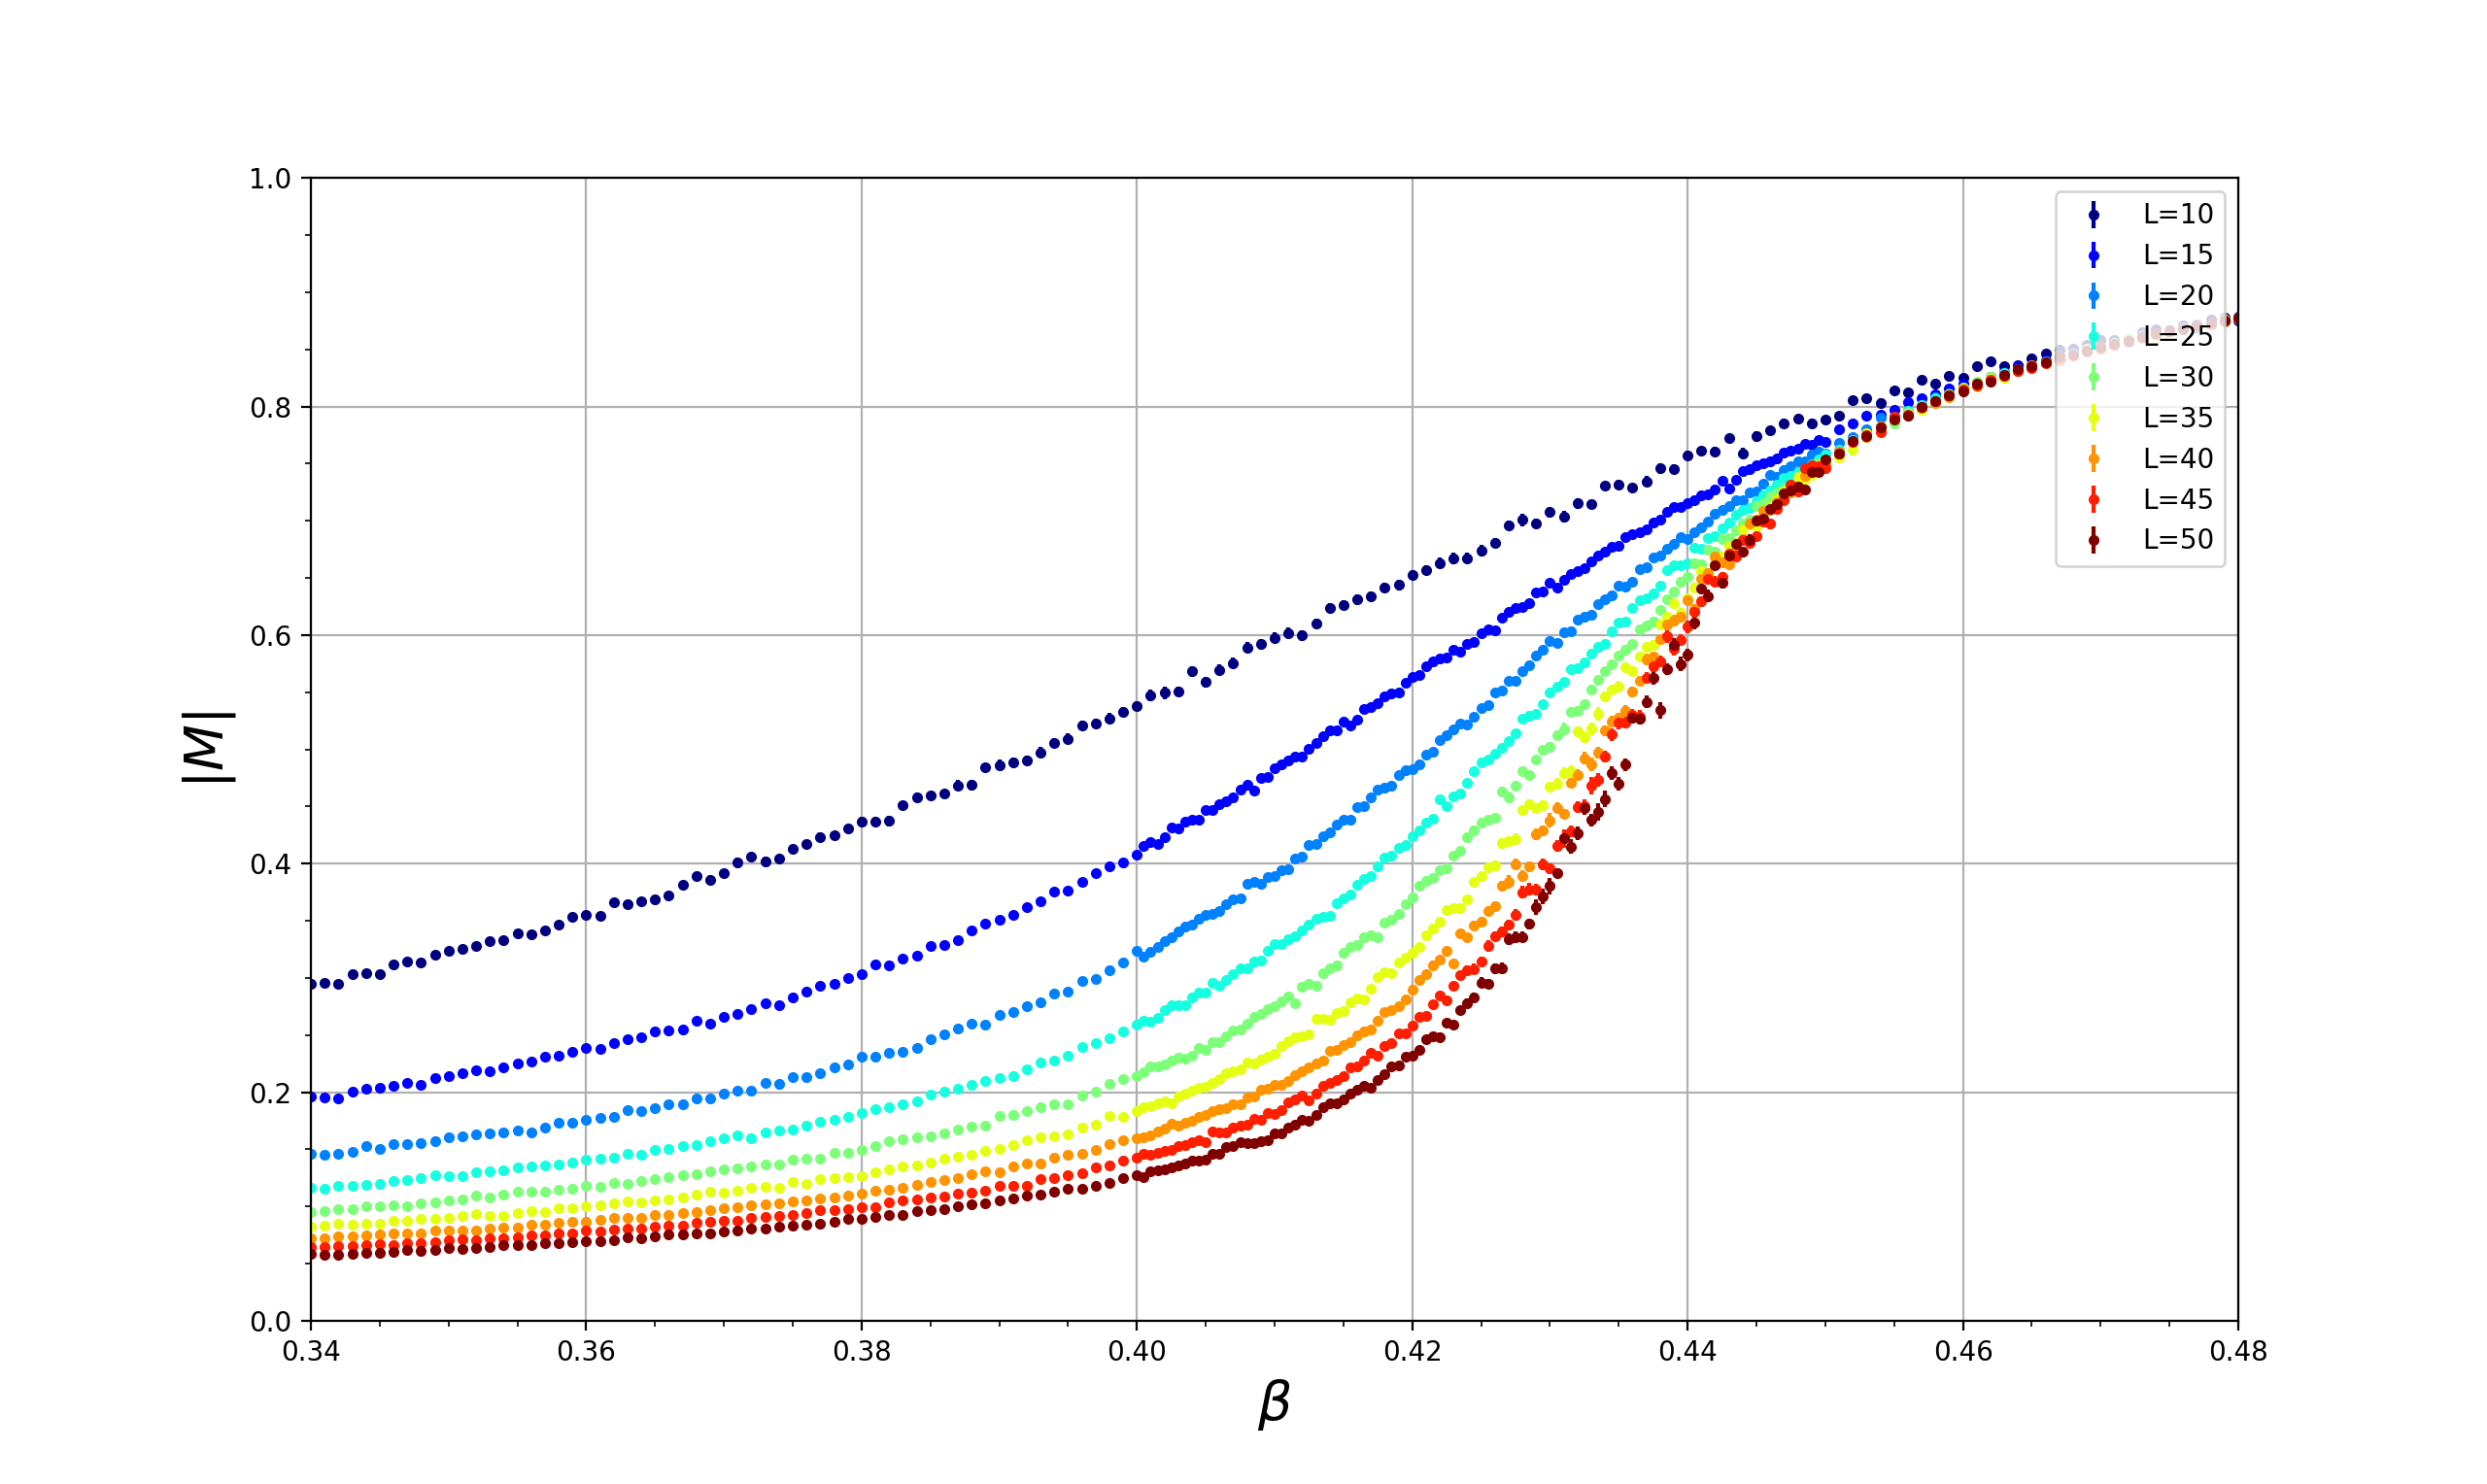
\includegraphics[width=1\linewidth]{magnass}
	\caption{Valor medio del valore assoluto della magnetizzazione al variare di $\beta$ per alcuni valori di $L$.}
	\label{fig:magnass}
\end{figure}
Si osservi che sopra la temperatura critica (ovvero per $\beta<\beta_c$) $\langle |M|\rangle$ non si annulla e diminuisce all'aumentare di $L$. Questo andamento è in accordo con l'andamento previsto per $T>T_c$ della distribuzione di probabilità della magnetizzazione $P(M)$: una gaussiana centrata in $M=0$ con larghezza che tende a $0$ come $1/L$ per $L\rightarrow\infty$. 

L'andamento sotto la temperatura critica è quello atteso: il sistema si magnetizza sempre di più all'aumentare di $\beta$ e risulta $\langle |M|\rangle\rightarrow 1$ per $\beta\rightarrow\infty$.
\subsection*{Ipotesi di scaling con $|M|$}
L'ipotesi di scaling implica l'esistenza di una funzione $\phi_M:\mathbb{R}\rightarrow\mathbb{R}$ tale che:\\
\begin{equation*}
|M(\beta,L)|= L^{-\beta/\nu}\phi_M\left((\beta-\beta_c)L^{\frac{1}{\nu}}\right)
\end{equation*}
E sostituendo i valori teorici degli esponenti critici:
\begin{equation*}
|M(\beta,L)| L^{1/8}=\phi_M\left((\beta-\beta_c)L\right)
\end{equation*}
Per verificare a posteriori l'ipotesi di scaling è sufficiente controllare il plot avente asse orizzontale $(\beta-\beta_c)L$ e asse verticale $|M| L^{1/8}$. Usando i valori di $|M|$ riportati in figura \ref{fig:magnass}, si ottiene il grafico in figura \ref{fig:magnFSS}.  


\begin{figure}[h!]%vedere cartella AbsMagnetizzazione
	\centering
	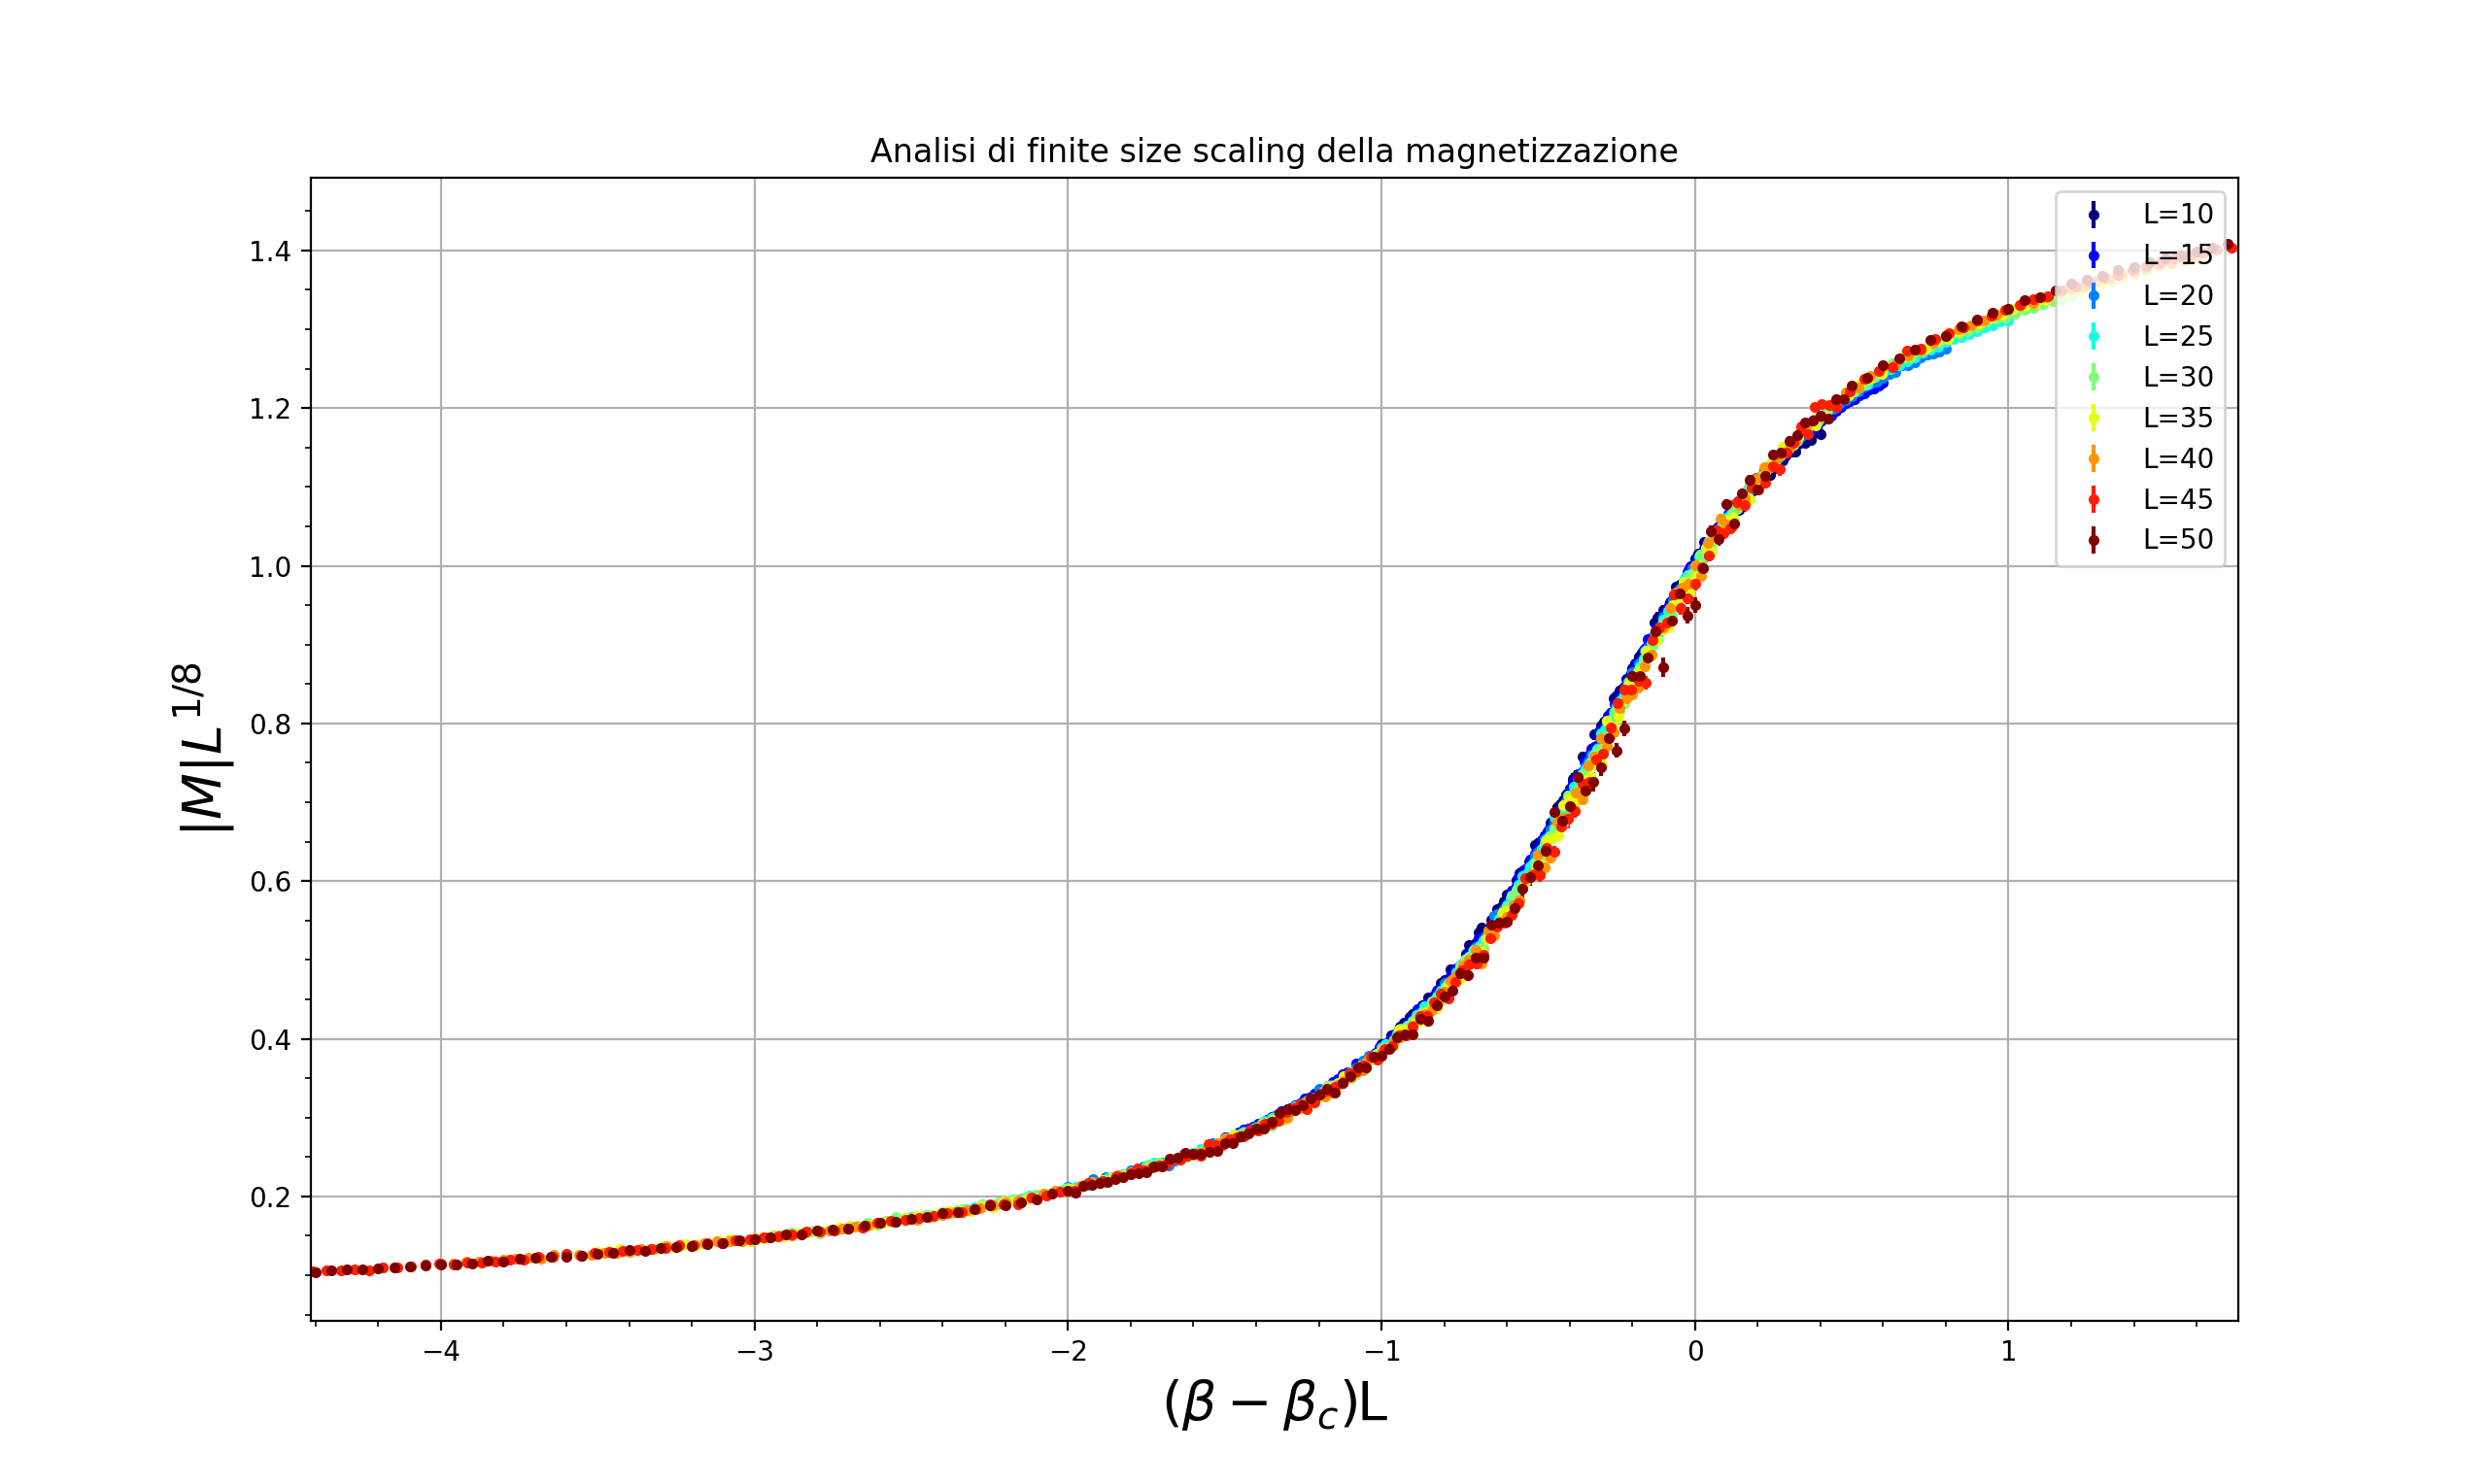
\includegraphics[width=1\linewidth]{magnass_norm}
	\caption{$|M|L^{\frac{1}{8}}$ in funzione della variabile di scaling $(\beta-\beta_c)L$.}
	\label{fig:magnFSS}
\end{figure}
Anche in questo caso, osservando il collasso dei punti su una sola curva, si conclude che l'ipotesi di scaling è verificata.

\newpage
\section{Osservazioni sul plot del calore specifico}
Il grafico del calore specifico $C$ in funzione di $\beta$ è riportato in figura \ref{fig:calspec}. 

\begin{figure}[h!] 
	\centering
	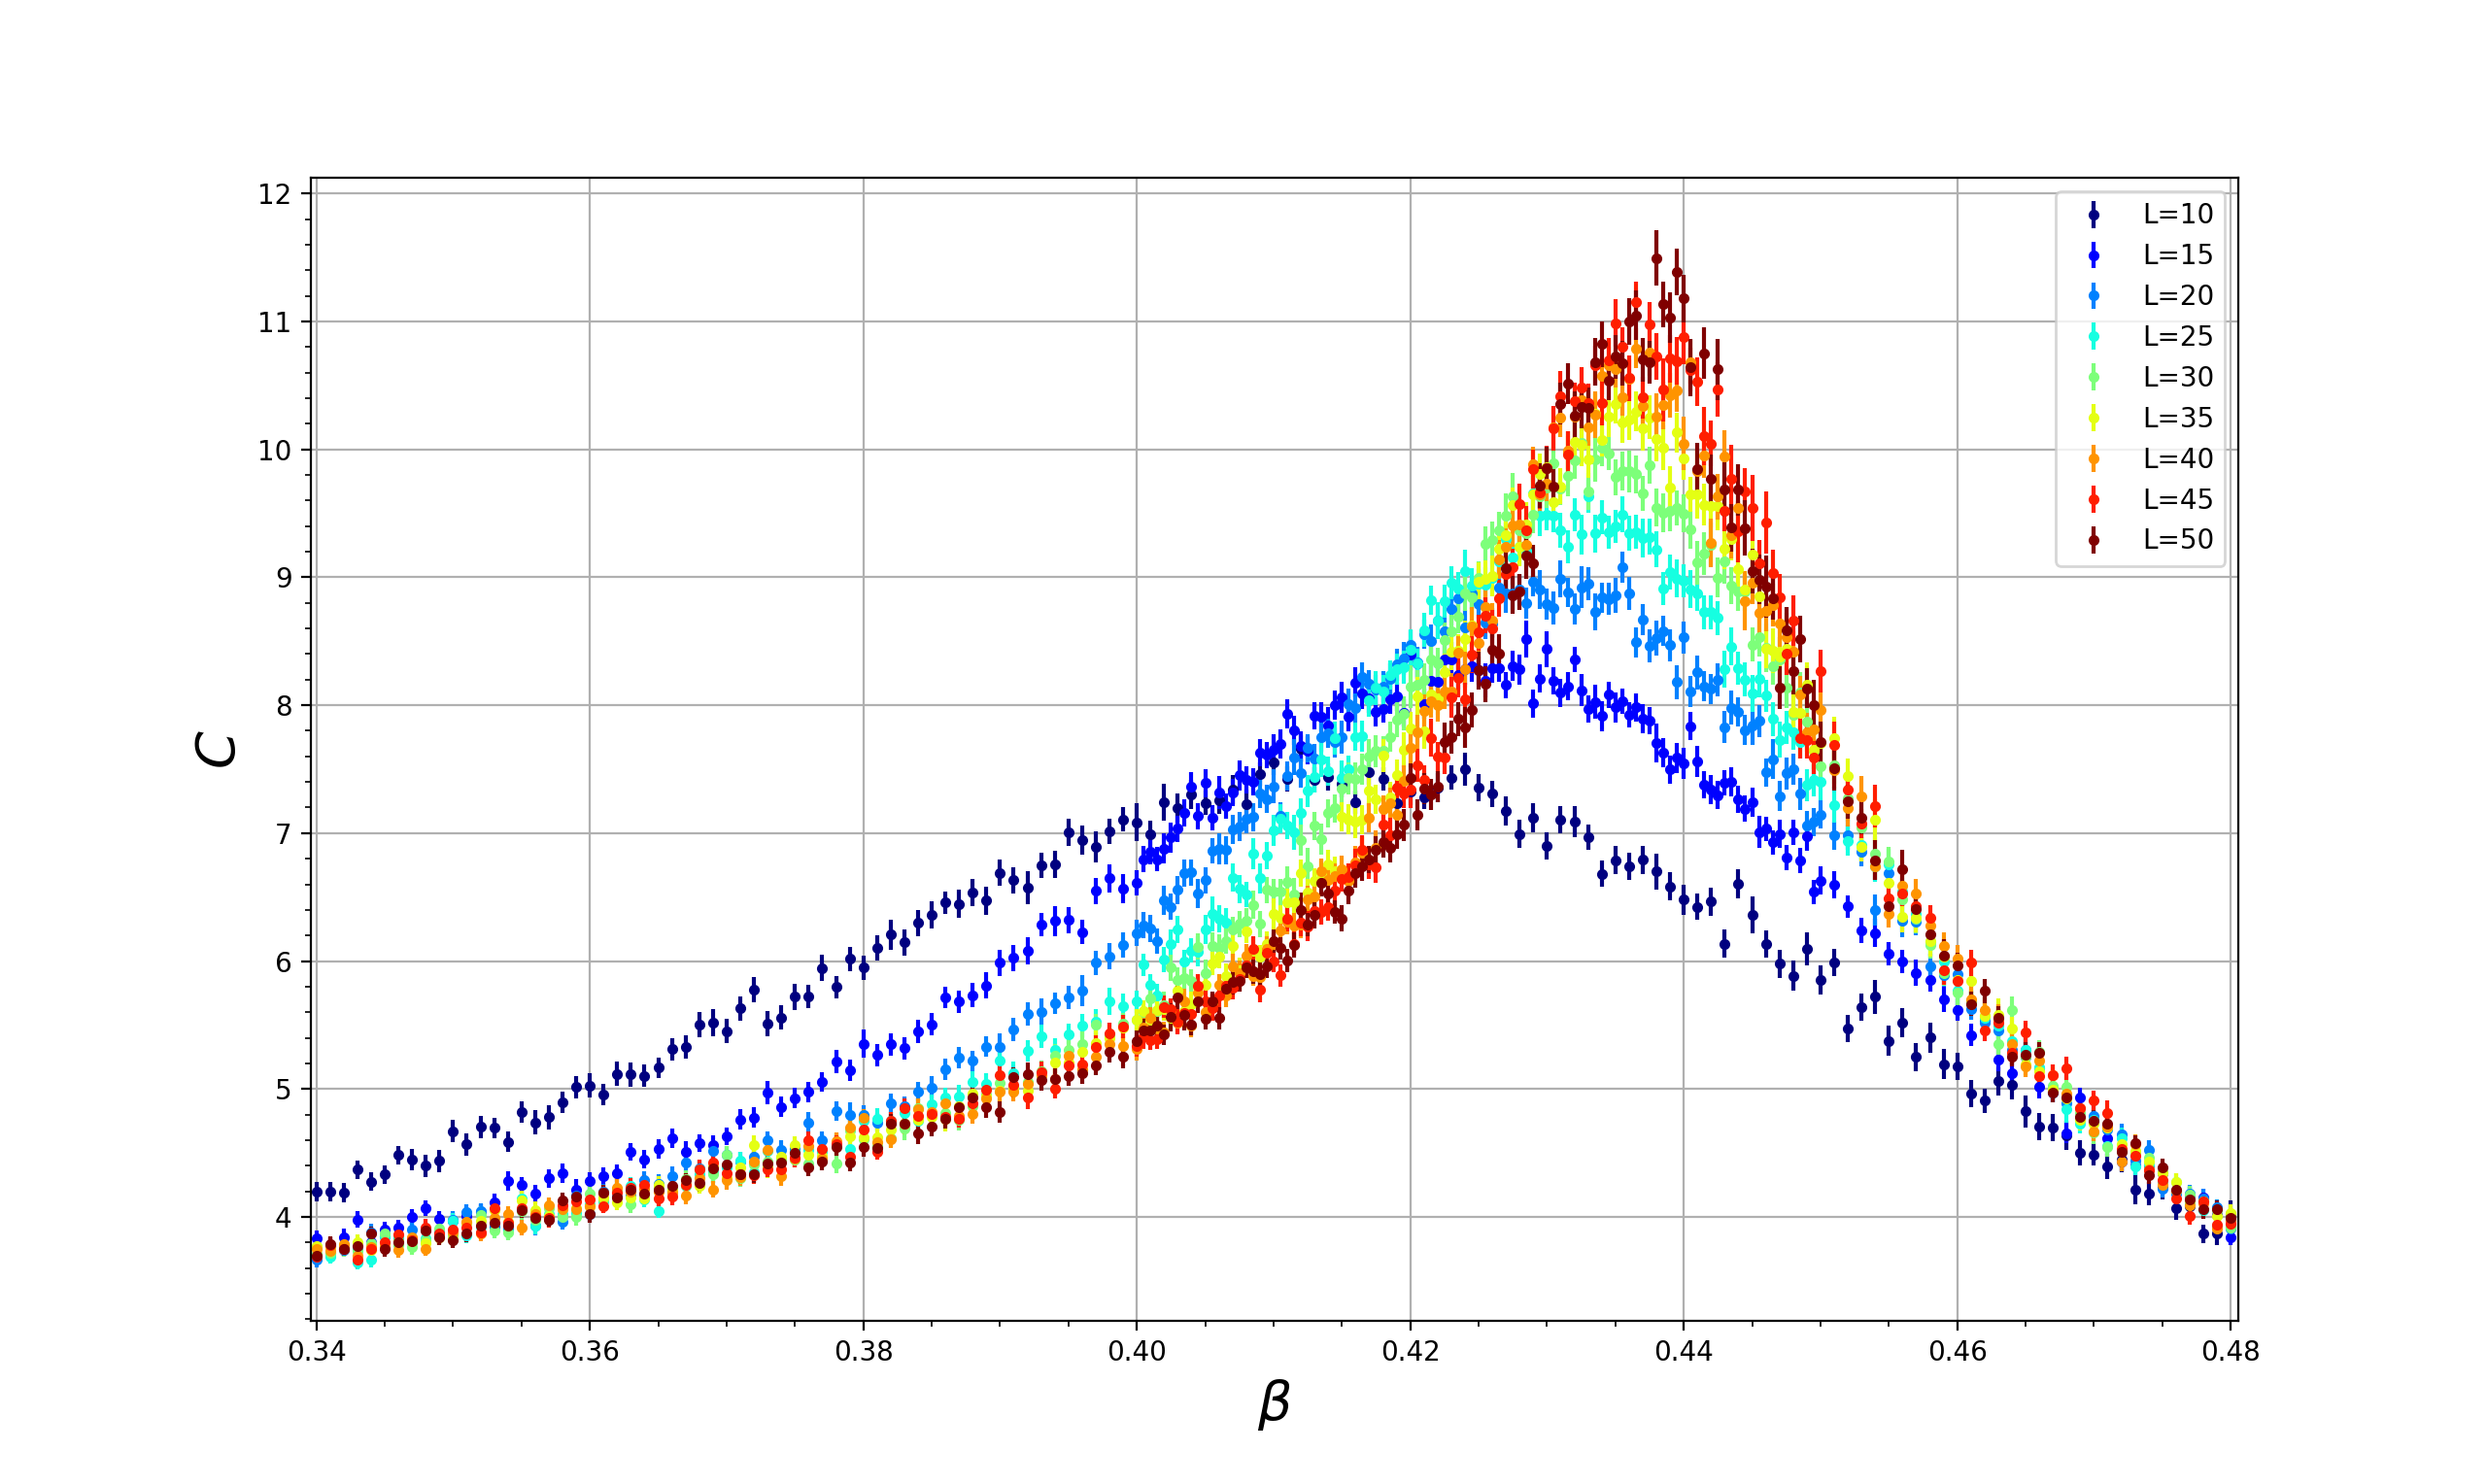
\includegraphics[width=1\linewidth]{calspec}
	\caption{Calore specifico al variare di $\beta$ per alcuni $L$.}
	\label{fig:calspec}
\end{figure}
\subsection*{Ipotesi di scaling con $C$}
Come in precedenza, l'ipotesi di scaling implica che esiste $\phi_C:\mathbb{R}\rightarrow\mathbb{R}$ tale che:\\
\begin{equation*}
C(\beta,L)= L^{\alpha/\nu}\phi_C((\beta-\beta_c)L^{\frac{1}{\nu}})
\end{equation*}
E sostituendo i valori teorici, si ottiene:
\begin{equation*}
C(\beta,L)=\phi_C((\beta-\beta_c)L^{\frac{1}{\nu}})
\end{equation*}
Il grafico, ottenuto come fatto in precedenza per $|M|$ e per $\chi$, è riportato in figura \ref{fig:calspecFSS}.

\begin{figure}[h!]
	\centering
	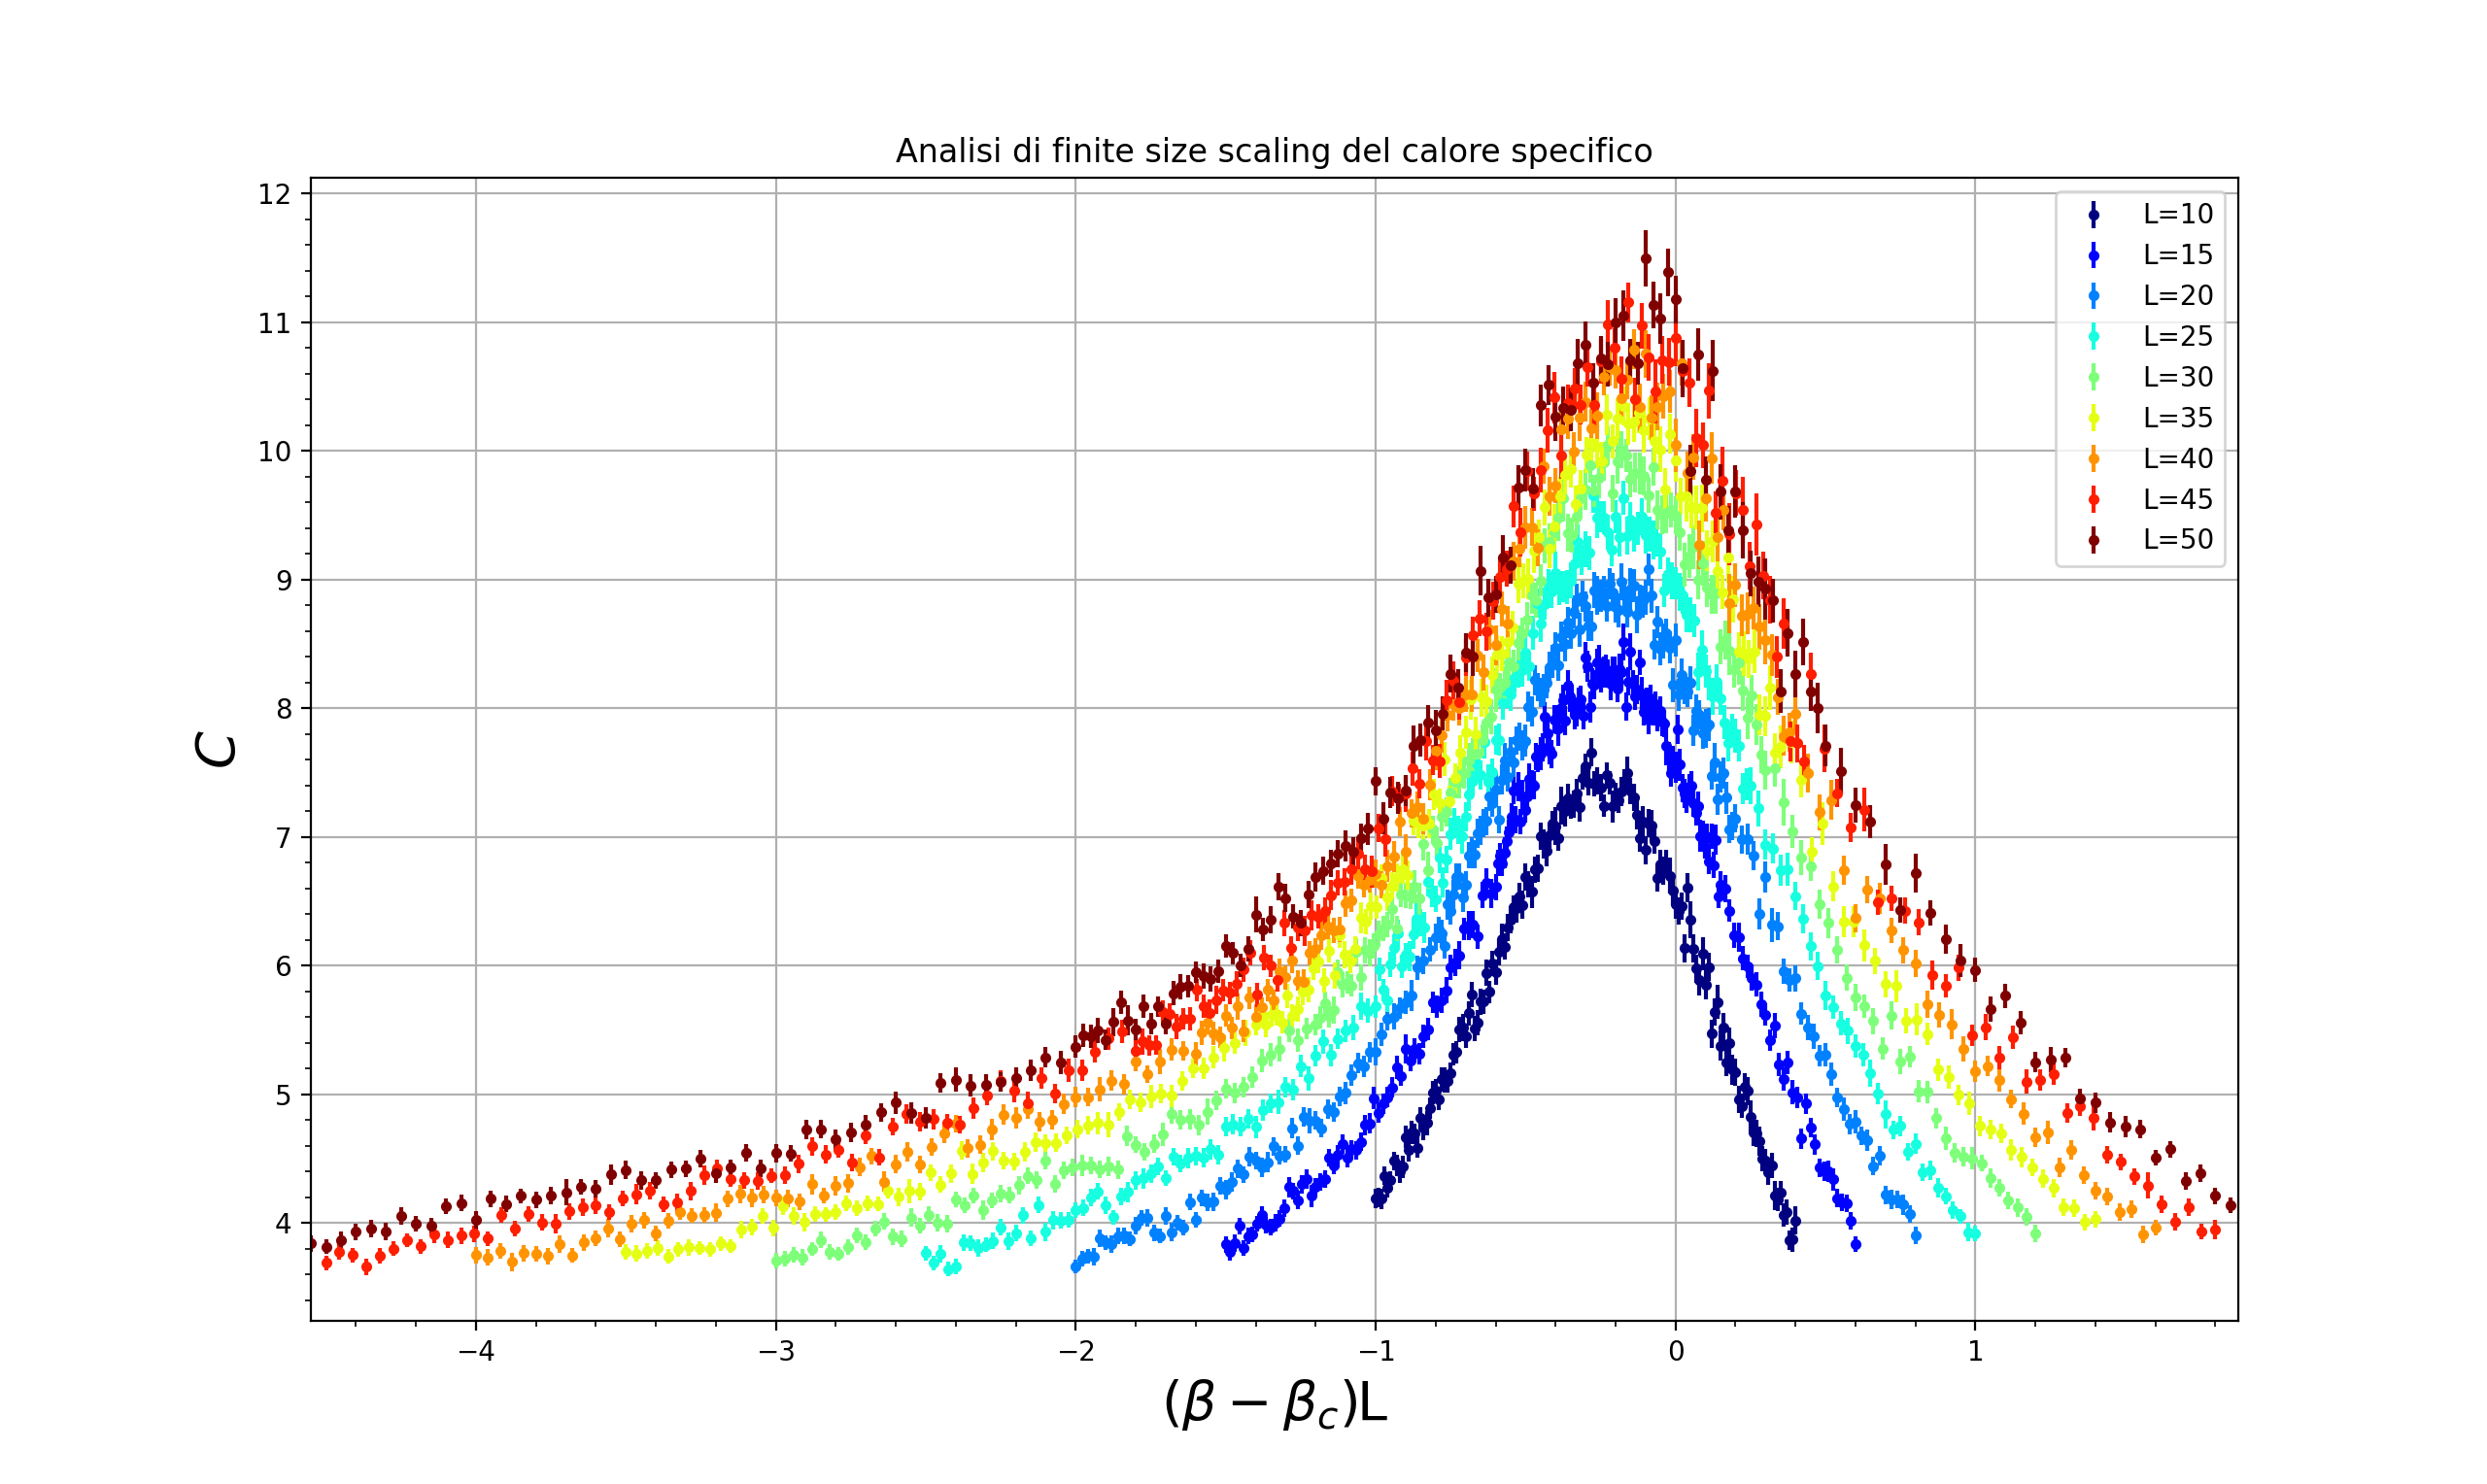
\includegraphics[width=1\linewidth]{cal_norm}
	\caption{$C$ in funzione della variabile di scaling $(\beta-\beta_c)L$.}
	\label{fig:calspecFSS}
\end{figure}

Questa volta l'ipotesi di scaling sembra non essere soddisfatta: le curve in figura \ref{fig:calspecFSS} non collassano su una sola curva. Si osservi, però, che le curve sembrano differenziarsi di una quantità indipendente da $\beta$. L'errore nel ragionamento precedente risiede nell'interpretazione del valore teorico $\alpha=0$. Il fatto che $\alpha$ valga $0$ non implica che avvicinandosi alla temperatura critica il calore specifico sia approssimativamente costante, bensì che cresca al più logaritmicamente. 

Il contributo logaritmico è stato tenuto in considerazione aggiungendo ad ogni curva una costante (diversa per ogni $L$) in modo da far coincidere i picchi. Questa correzione è riportata in figura \ref{fig:calspecFSScorr}.
\begin{figure}[h!]
	\centering
	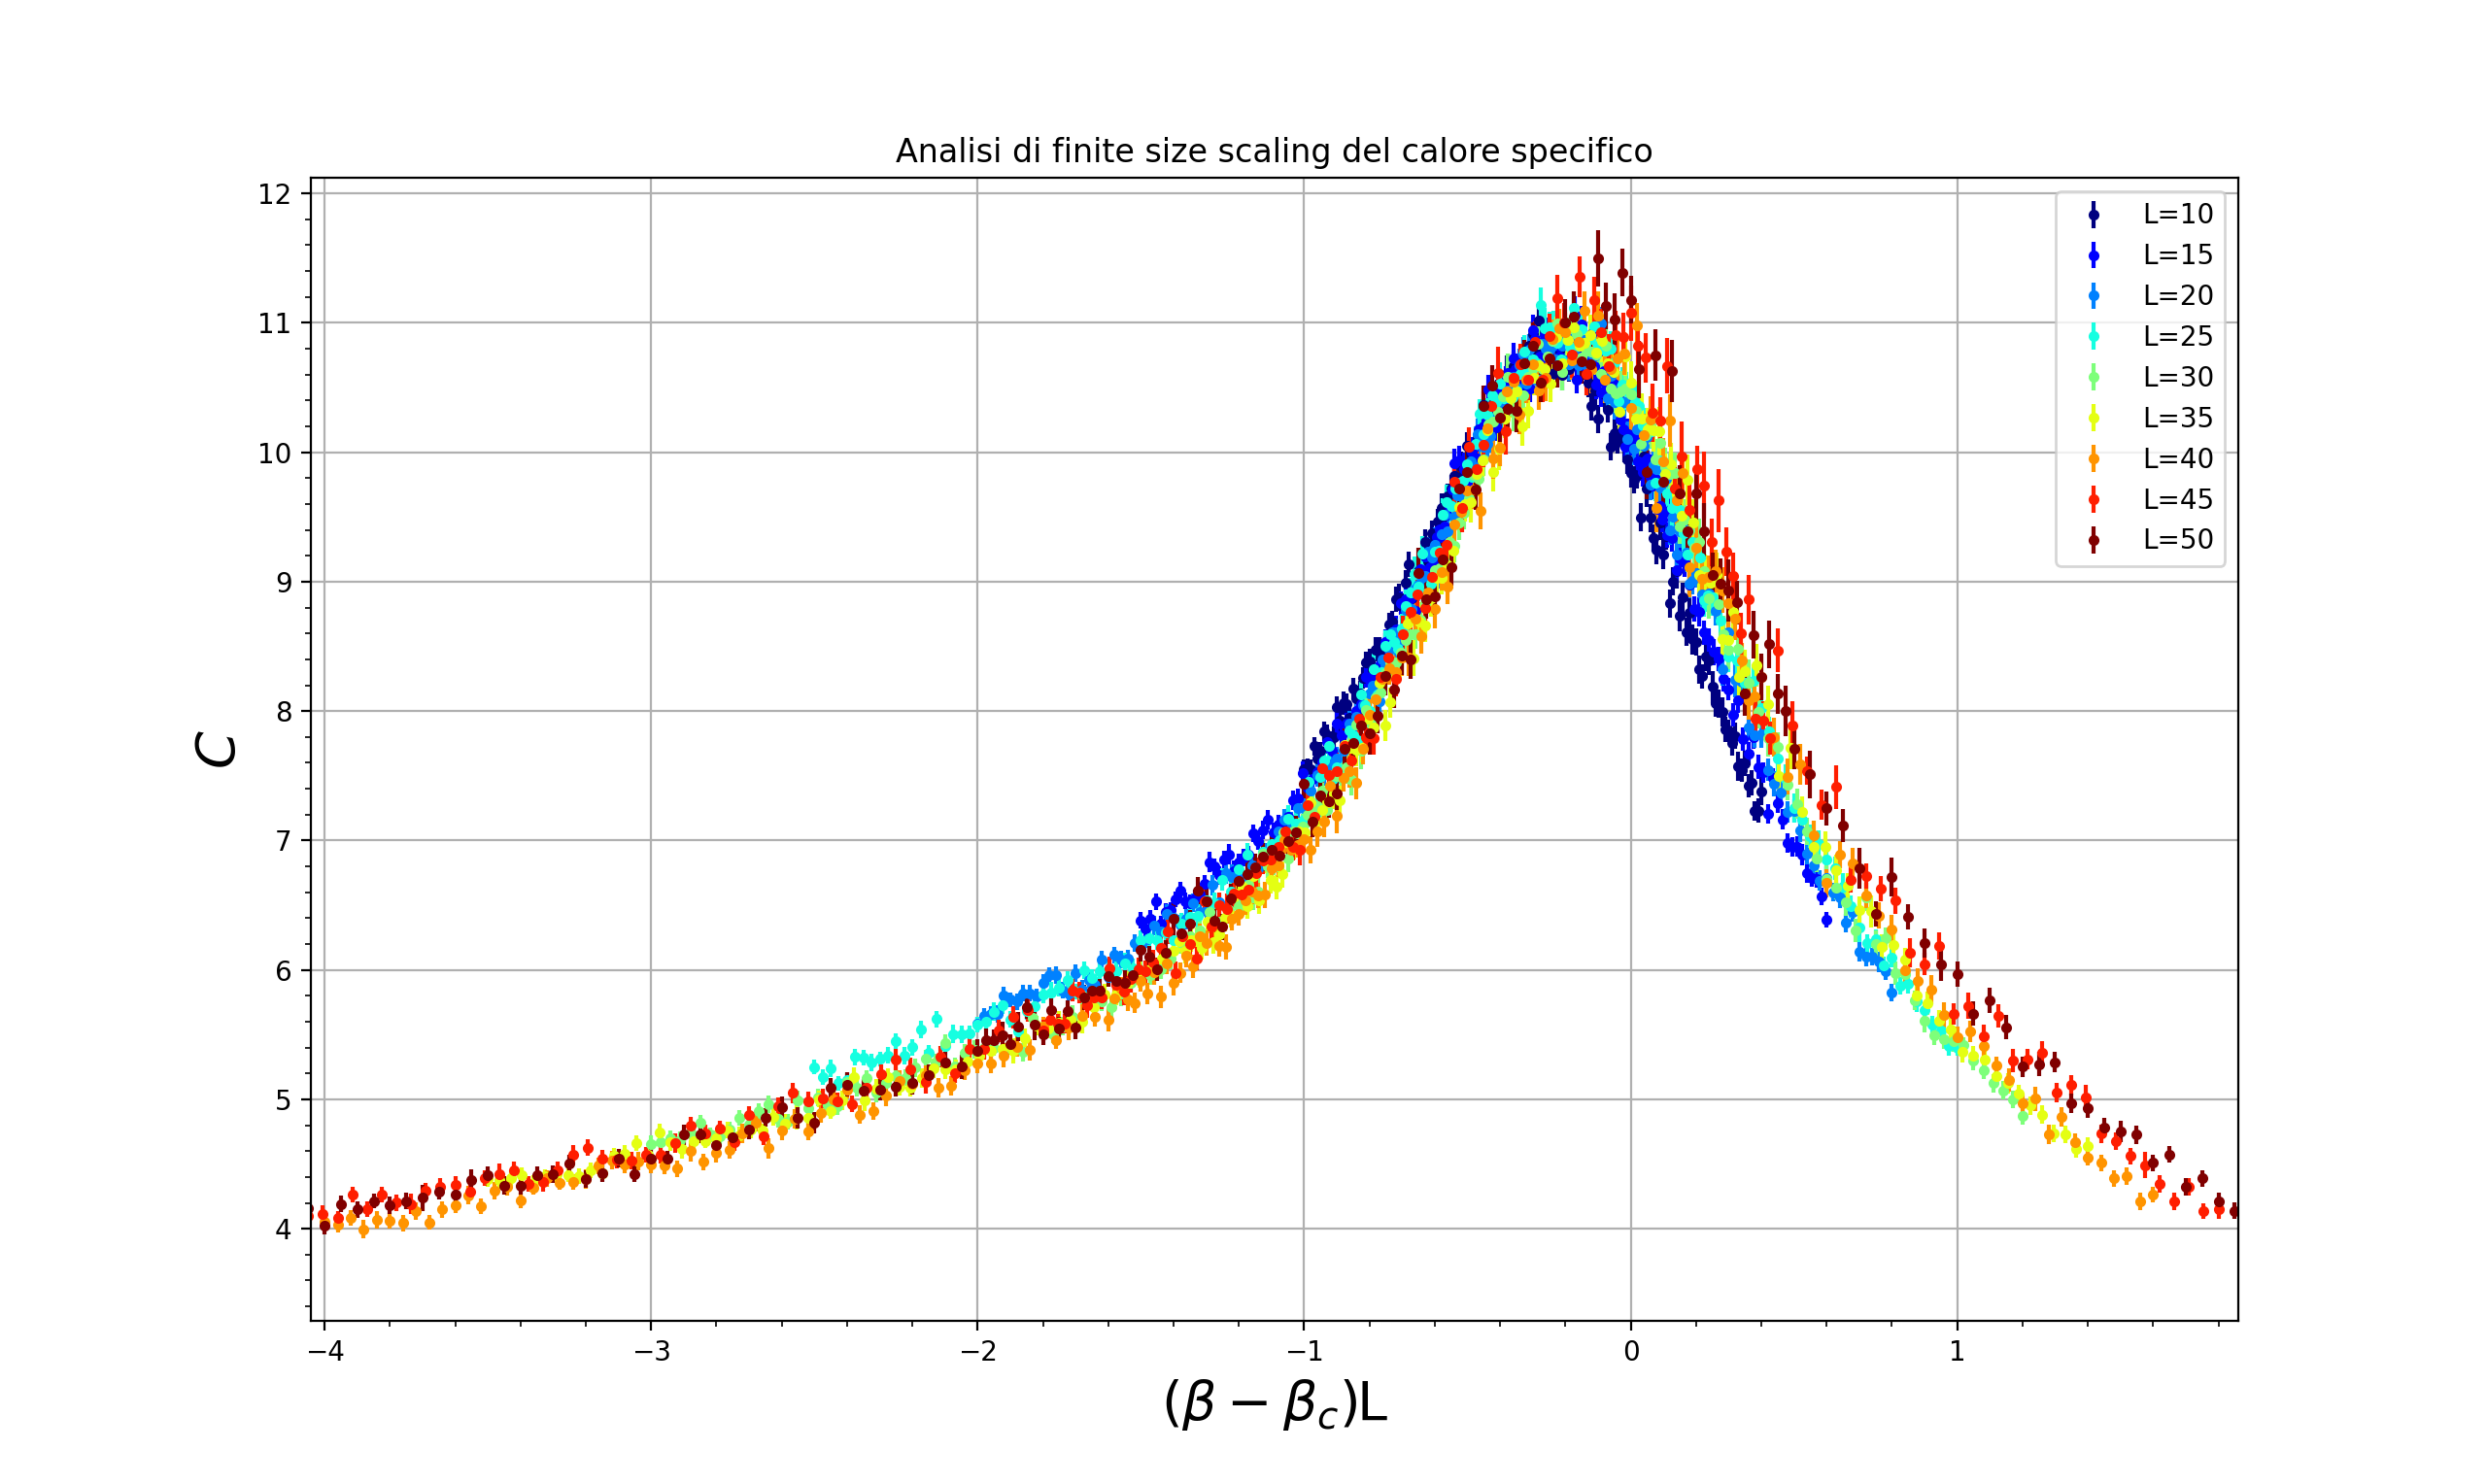
\includegraphics[width=1\linewidth]{cal_corr}
	\caption{$C$ + "correzioni" in funzione della variabile di scaling $(\beta-\beta_c)L$.}
	\label{fig:calspecFSScorr}
\end{figure}

Dalla figura \ref{fig:calspecFSScorr} si deduce che l'ipotesi di scaling risulta nuovamente salva.


\section{Energia per sito e cumulante di Binder}
Per completezza, riportiamo anche i grafici dell'energia per sito $\epsilon$ e del cumulante di Binder $B$ al variare di $\beta$ rispettivamente in figura \ref{ene} e in figura \ref{binder}.
\begin{figure}[h!]
	\centering
	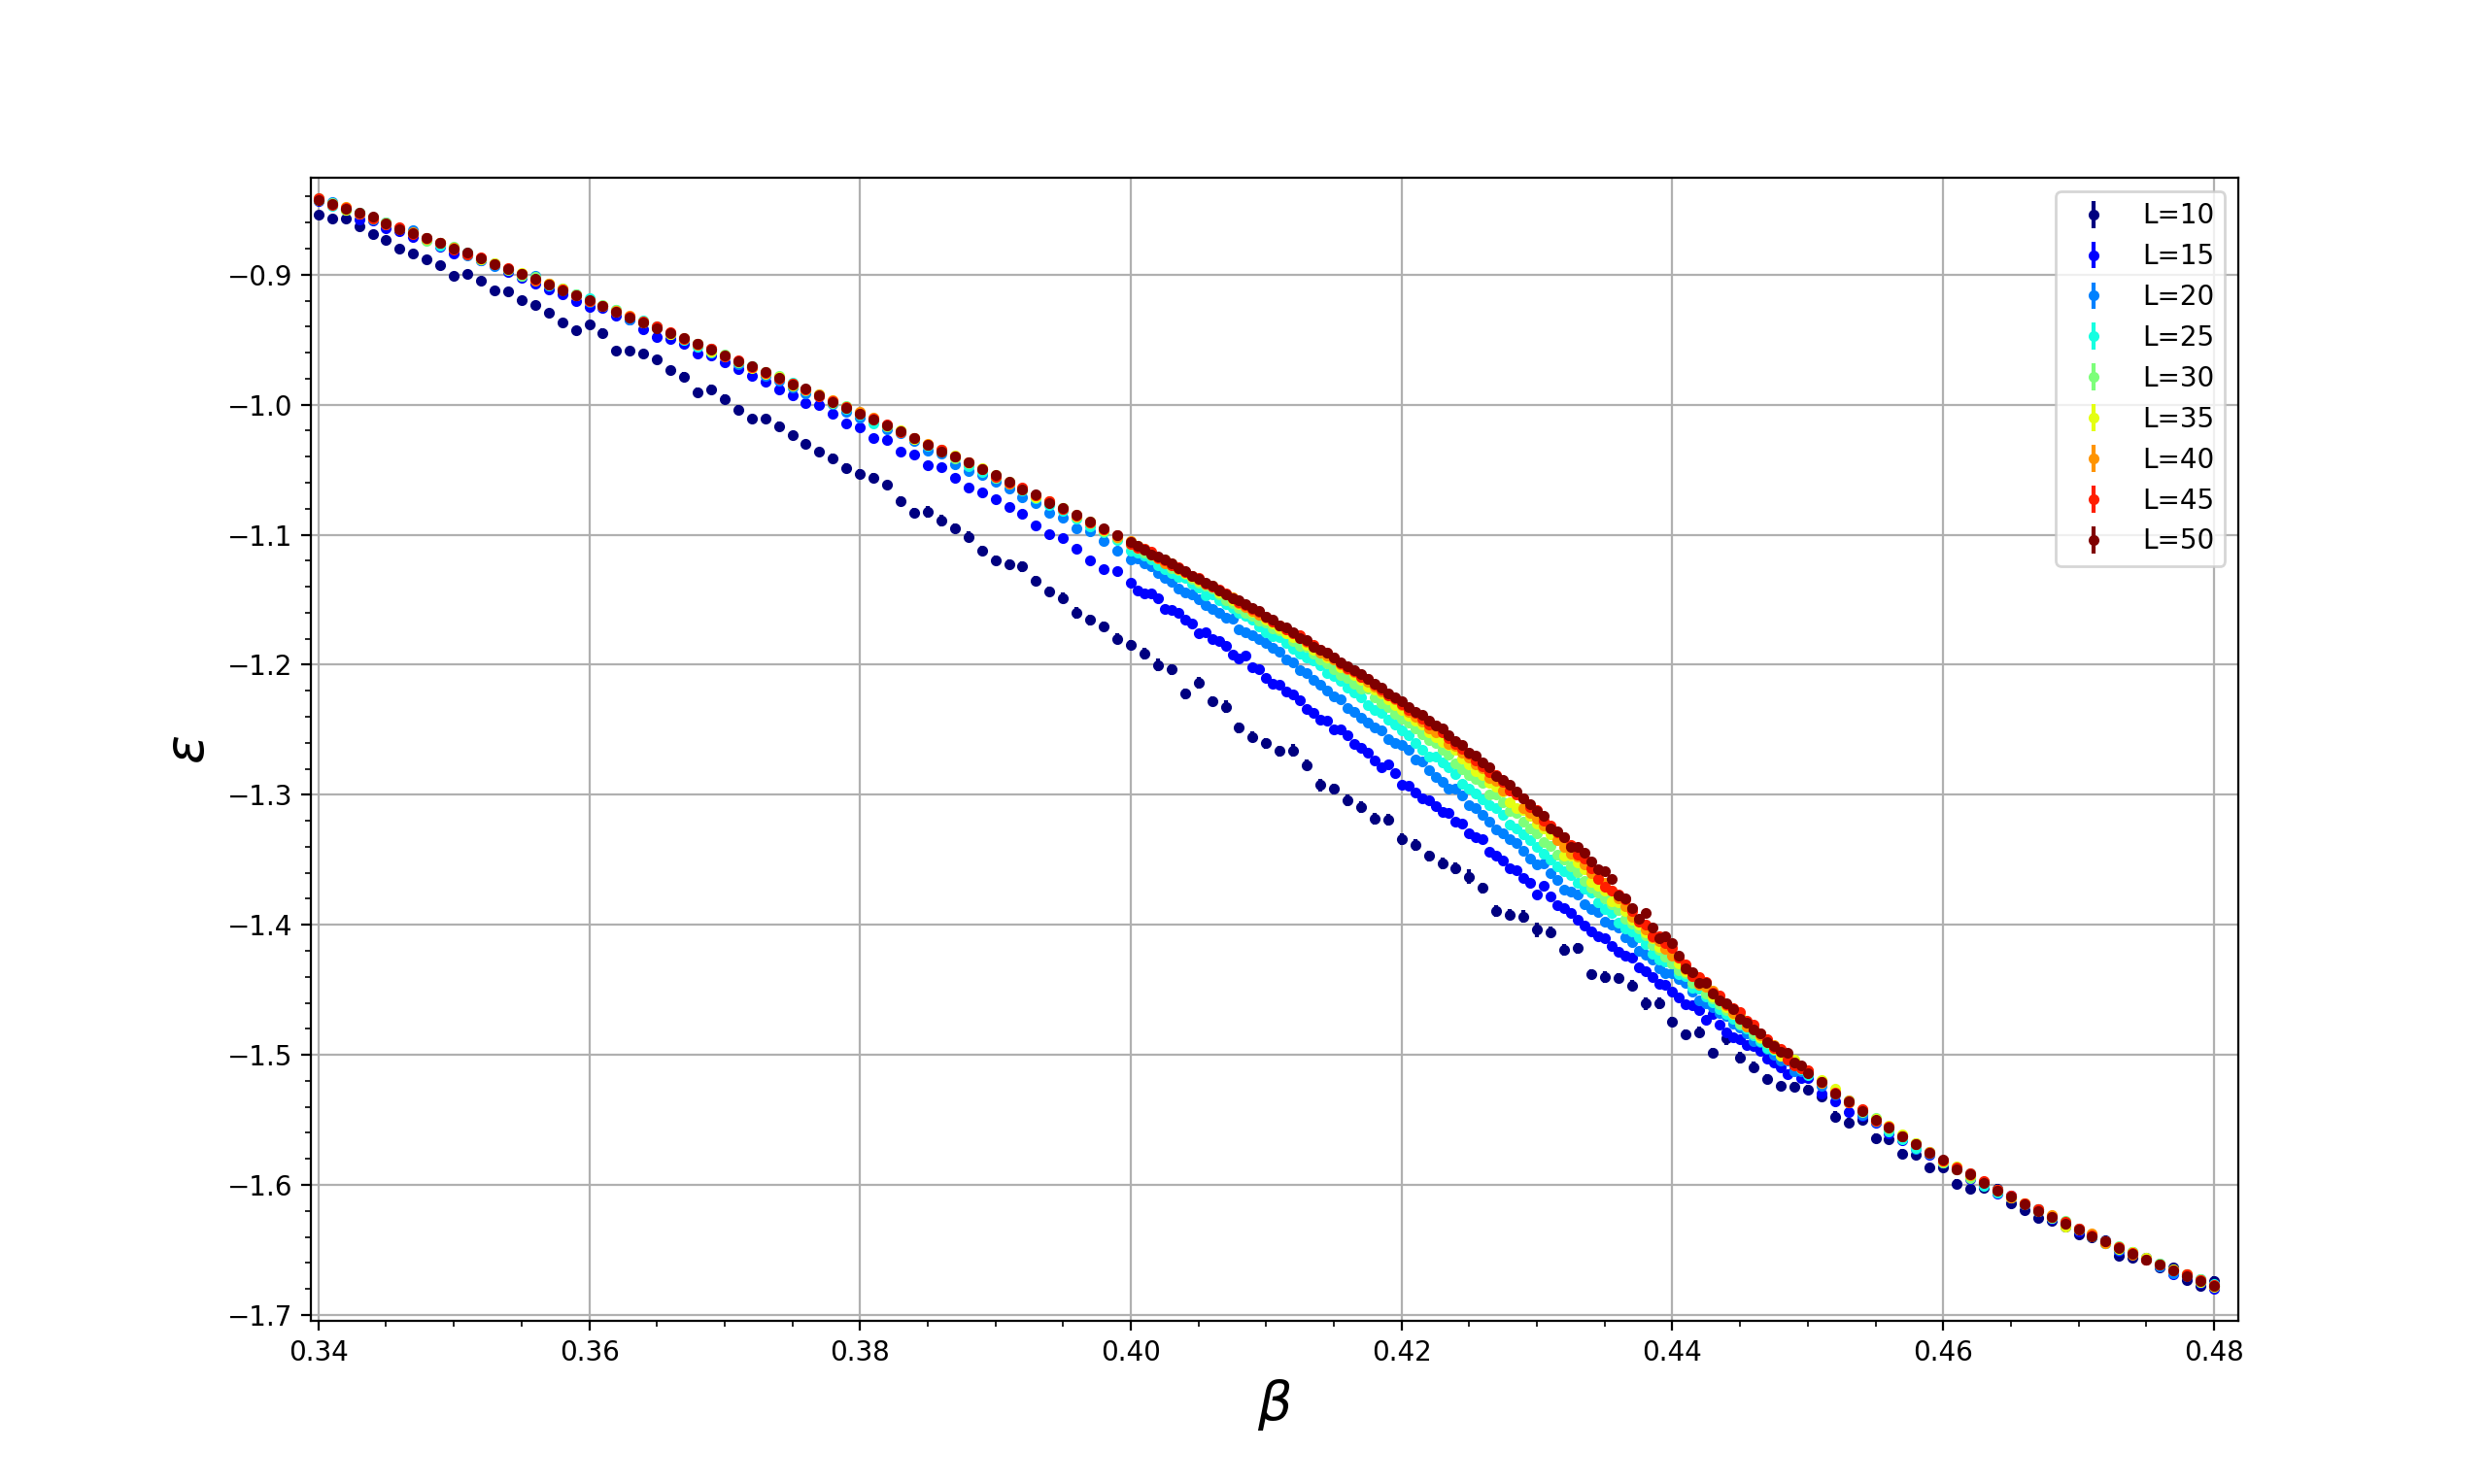
\includegraphics[width=1\linewidth]{ene}
	\caption{Energia media per sito al variare di $\beta$ per alcuni $L$.}
	\label{ene}
\end{figure}
\begin{figure}[h!]
	\centering
	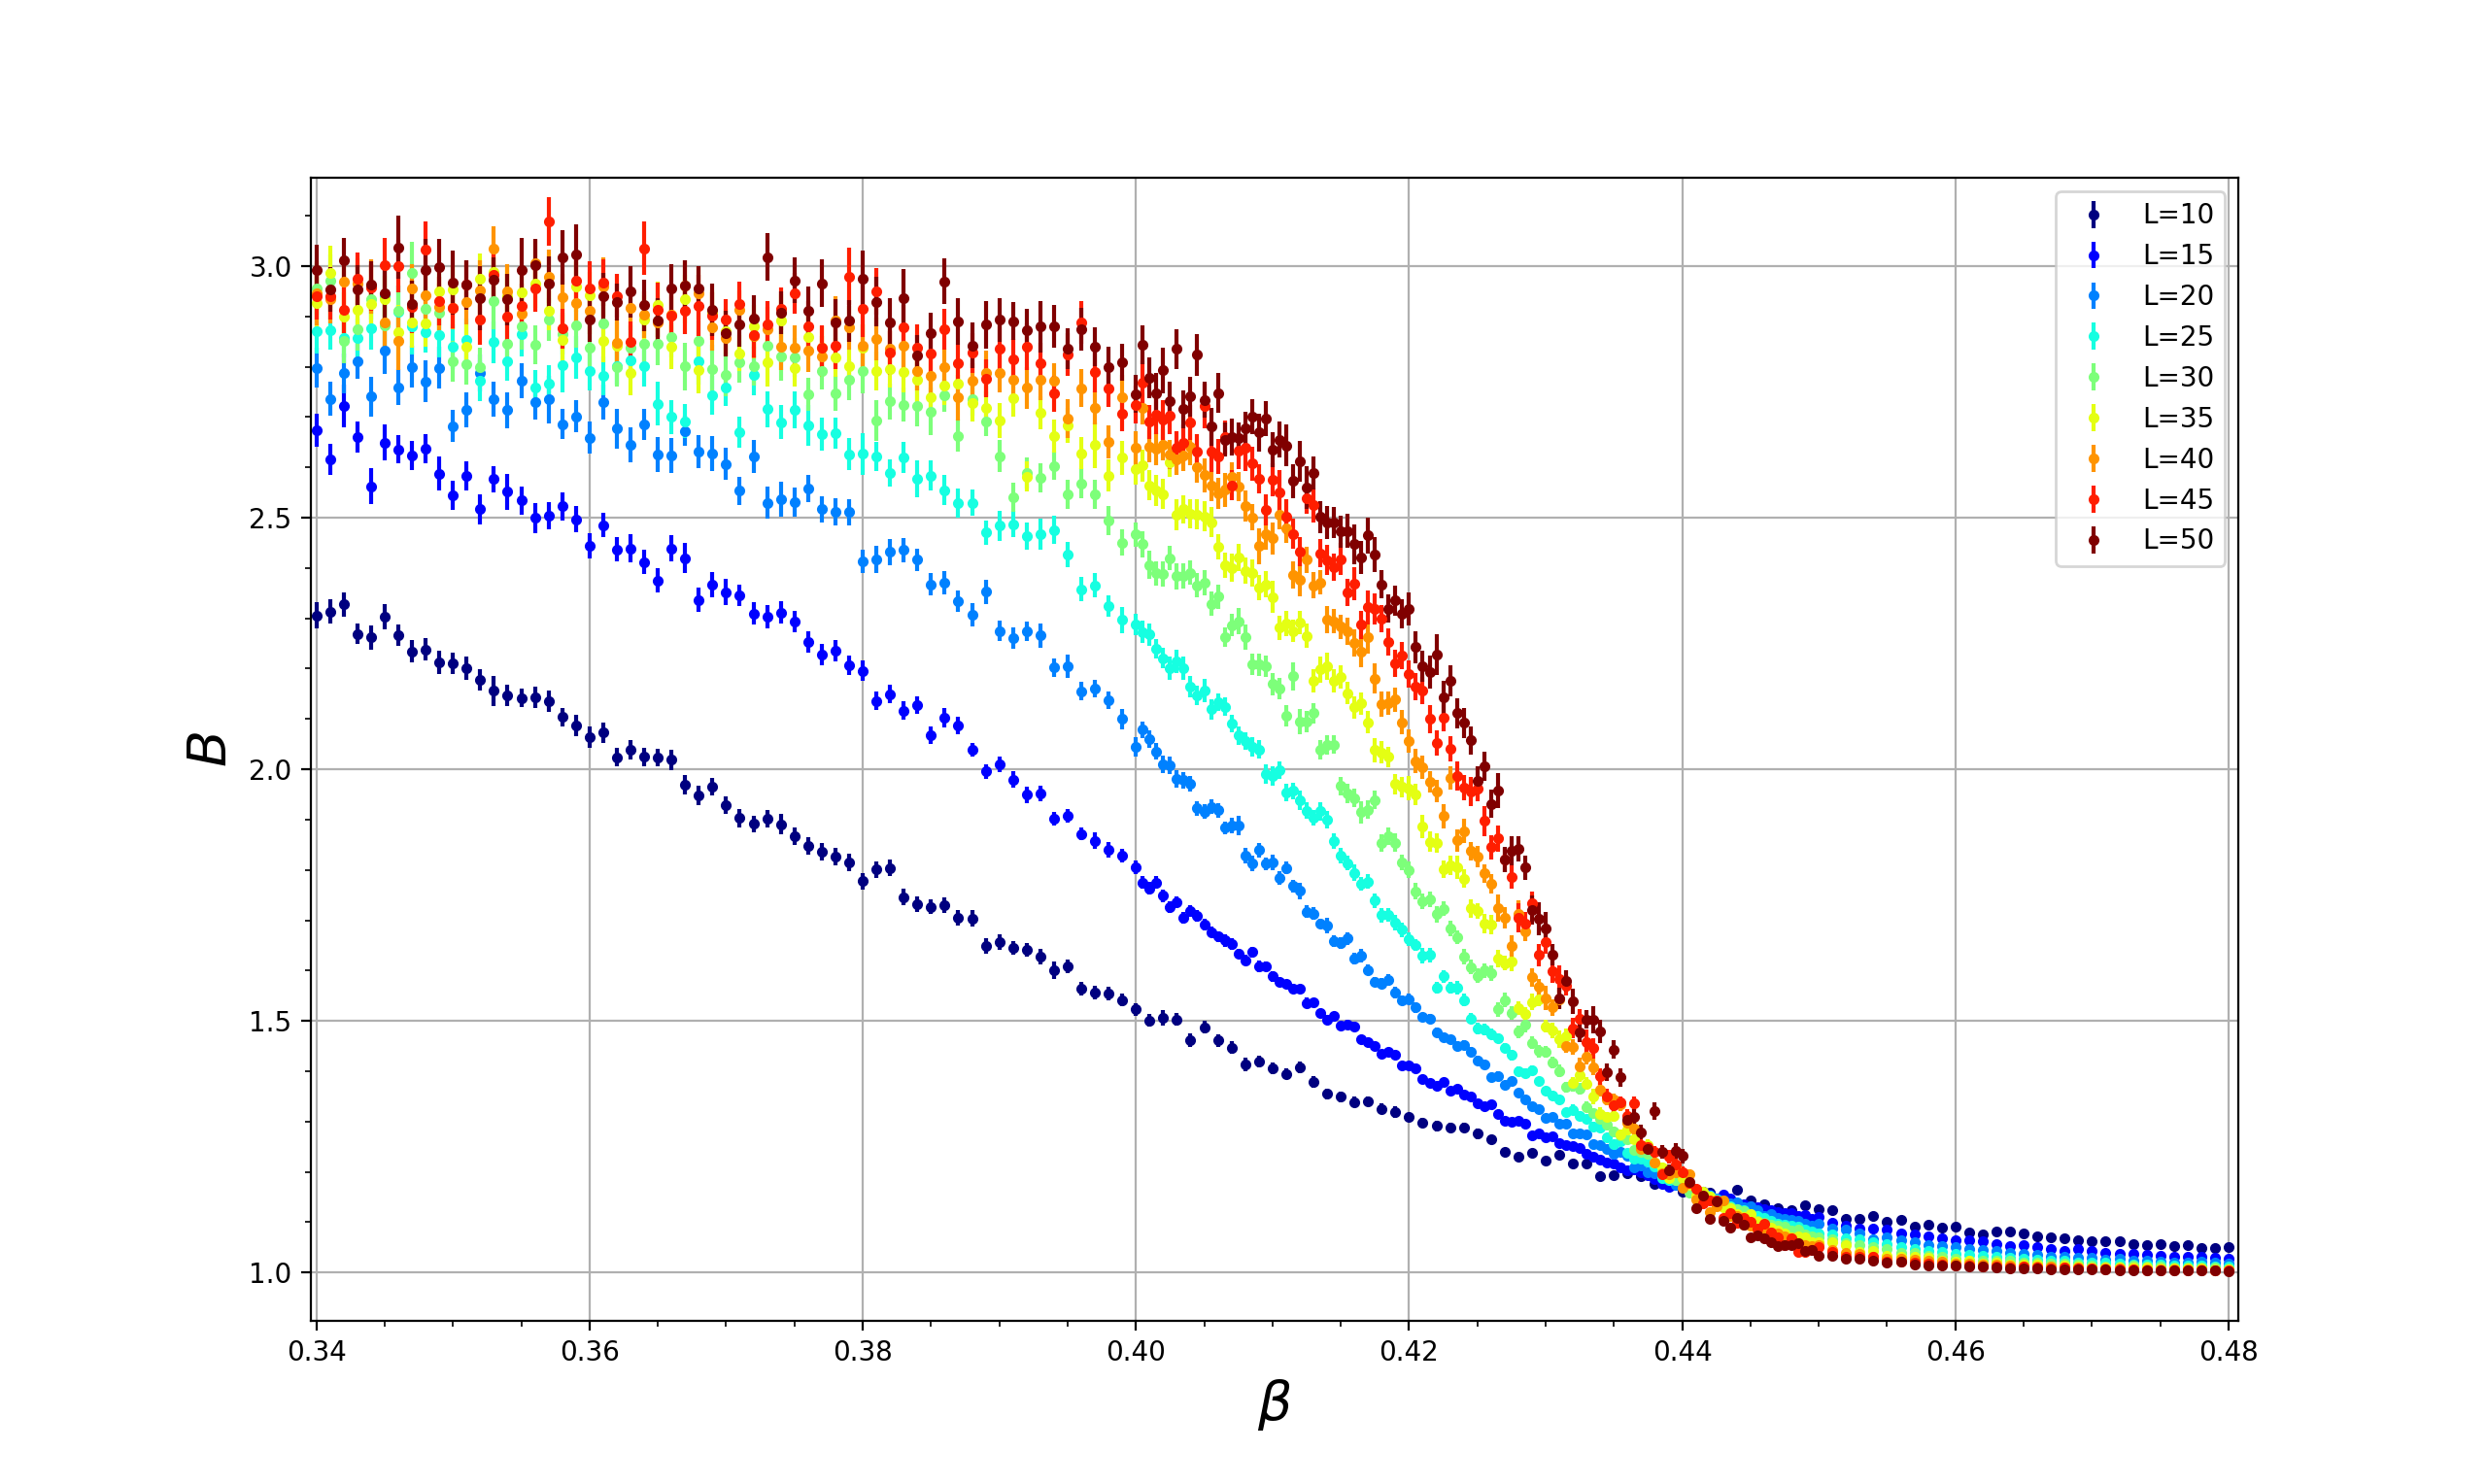
\includegraphics[width=1\linewidth]{binder}
	\caption{Cumulante di Binder al variare di $\beta$ per alcuni $L$.}
	\label{binder}
\end{figure}


\newpage
\section{Secondo modo per stimare $\gamma$}
In questa sezione viene spiegato un altro modo per stimare $\gamma$. 
Nel caso di reticolo infinito, il comportamento critico della suscettività è:
\begin{equation}
	\chi \sim |t|^{-\gamma}
	\label{eq:suscand}
\end{equation}
Inoltre per $\beta$ vicino a $\beta_c$, si ha:
\begin{equation}\label{approxt} t\coloneqq\frac{T-T_c}{T_c}\sim1-\frac{\beta}{\beta_c}
\end{equation}
La strategia è fare un fit della suscettività in un intervallo che sia:
\begin{itemize}
	\item sufficientemente lontano da $\beta_c$ in modo tale che non emergano effetti di reticolo finito;\footnote{Gli effetti di reticolo finito emergono quando la lunghezza di correlazione $\xi$ è confrontabile con $L$.}
	\item sufficientemente vicino a $\beta_c$ in modo tale che risulti ragionevole l'approssimazione $\chi\sim |t|^{-\gamma}$.
\end{itemize}  
E' stata scelta la curva in figura \ref{suscettivitabeta} corrispondente al reticolo più lungo su cui è stata misurata $\chi$, cioè quella con $L=50$. Prendendo il logaritmo dell'espressione \ref{eq:suscand} e usando l'equazione \ref{approxt}, si ha:
\begin{equation}\label{eqfit}
\log\chi \sim -\gamma \log|t| \sim -\gamma \log|1-\frac{\beta}{\beta_c}|
\end{equation}
dove per $\beta_c$ si intende il punto di massimo della curva con $L=50$, ovvero $\beta_{pc}(L=50)$.


L'intervallo utilizzato per bilanciare al meglio le due precedenti condizioni è $\beta\in[0.4390,0.4515]$. Il punto di massimo $\beta_{pc}(L=50)$ era stato già stimato in tabella \ref{suscmax} e vale $\beta_{pc}(L=50)=0.4324\pm0003$.

In virtù dell'equazione \ref{eqfit}, come funzione di fit è stata scelta una retta $f(x)\coloneqq a-\gamma x$, dove $x$ corrisponde alla variabile $\log|t|=\log(-1+\frac{\beta}{\beta_{pc}})$ (il segno è questo in quanto l'intervallo utilizzato si trova a destra di $\beta_{pc}$). Il risultato del fit è:%vedere cartella StimaGamma
 $$\gamma=1.76\pm0.11$$ il che è in accordo con le aspettative. Il chi quadro ridotto è di $4.2$ .

%Il plot con la retta di best fit è riportata in figura \ref{fig:gammadx}.\\
%\begin{figure}[h!]
%	\centering
%	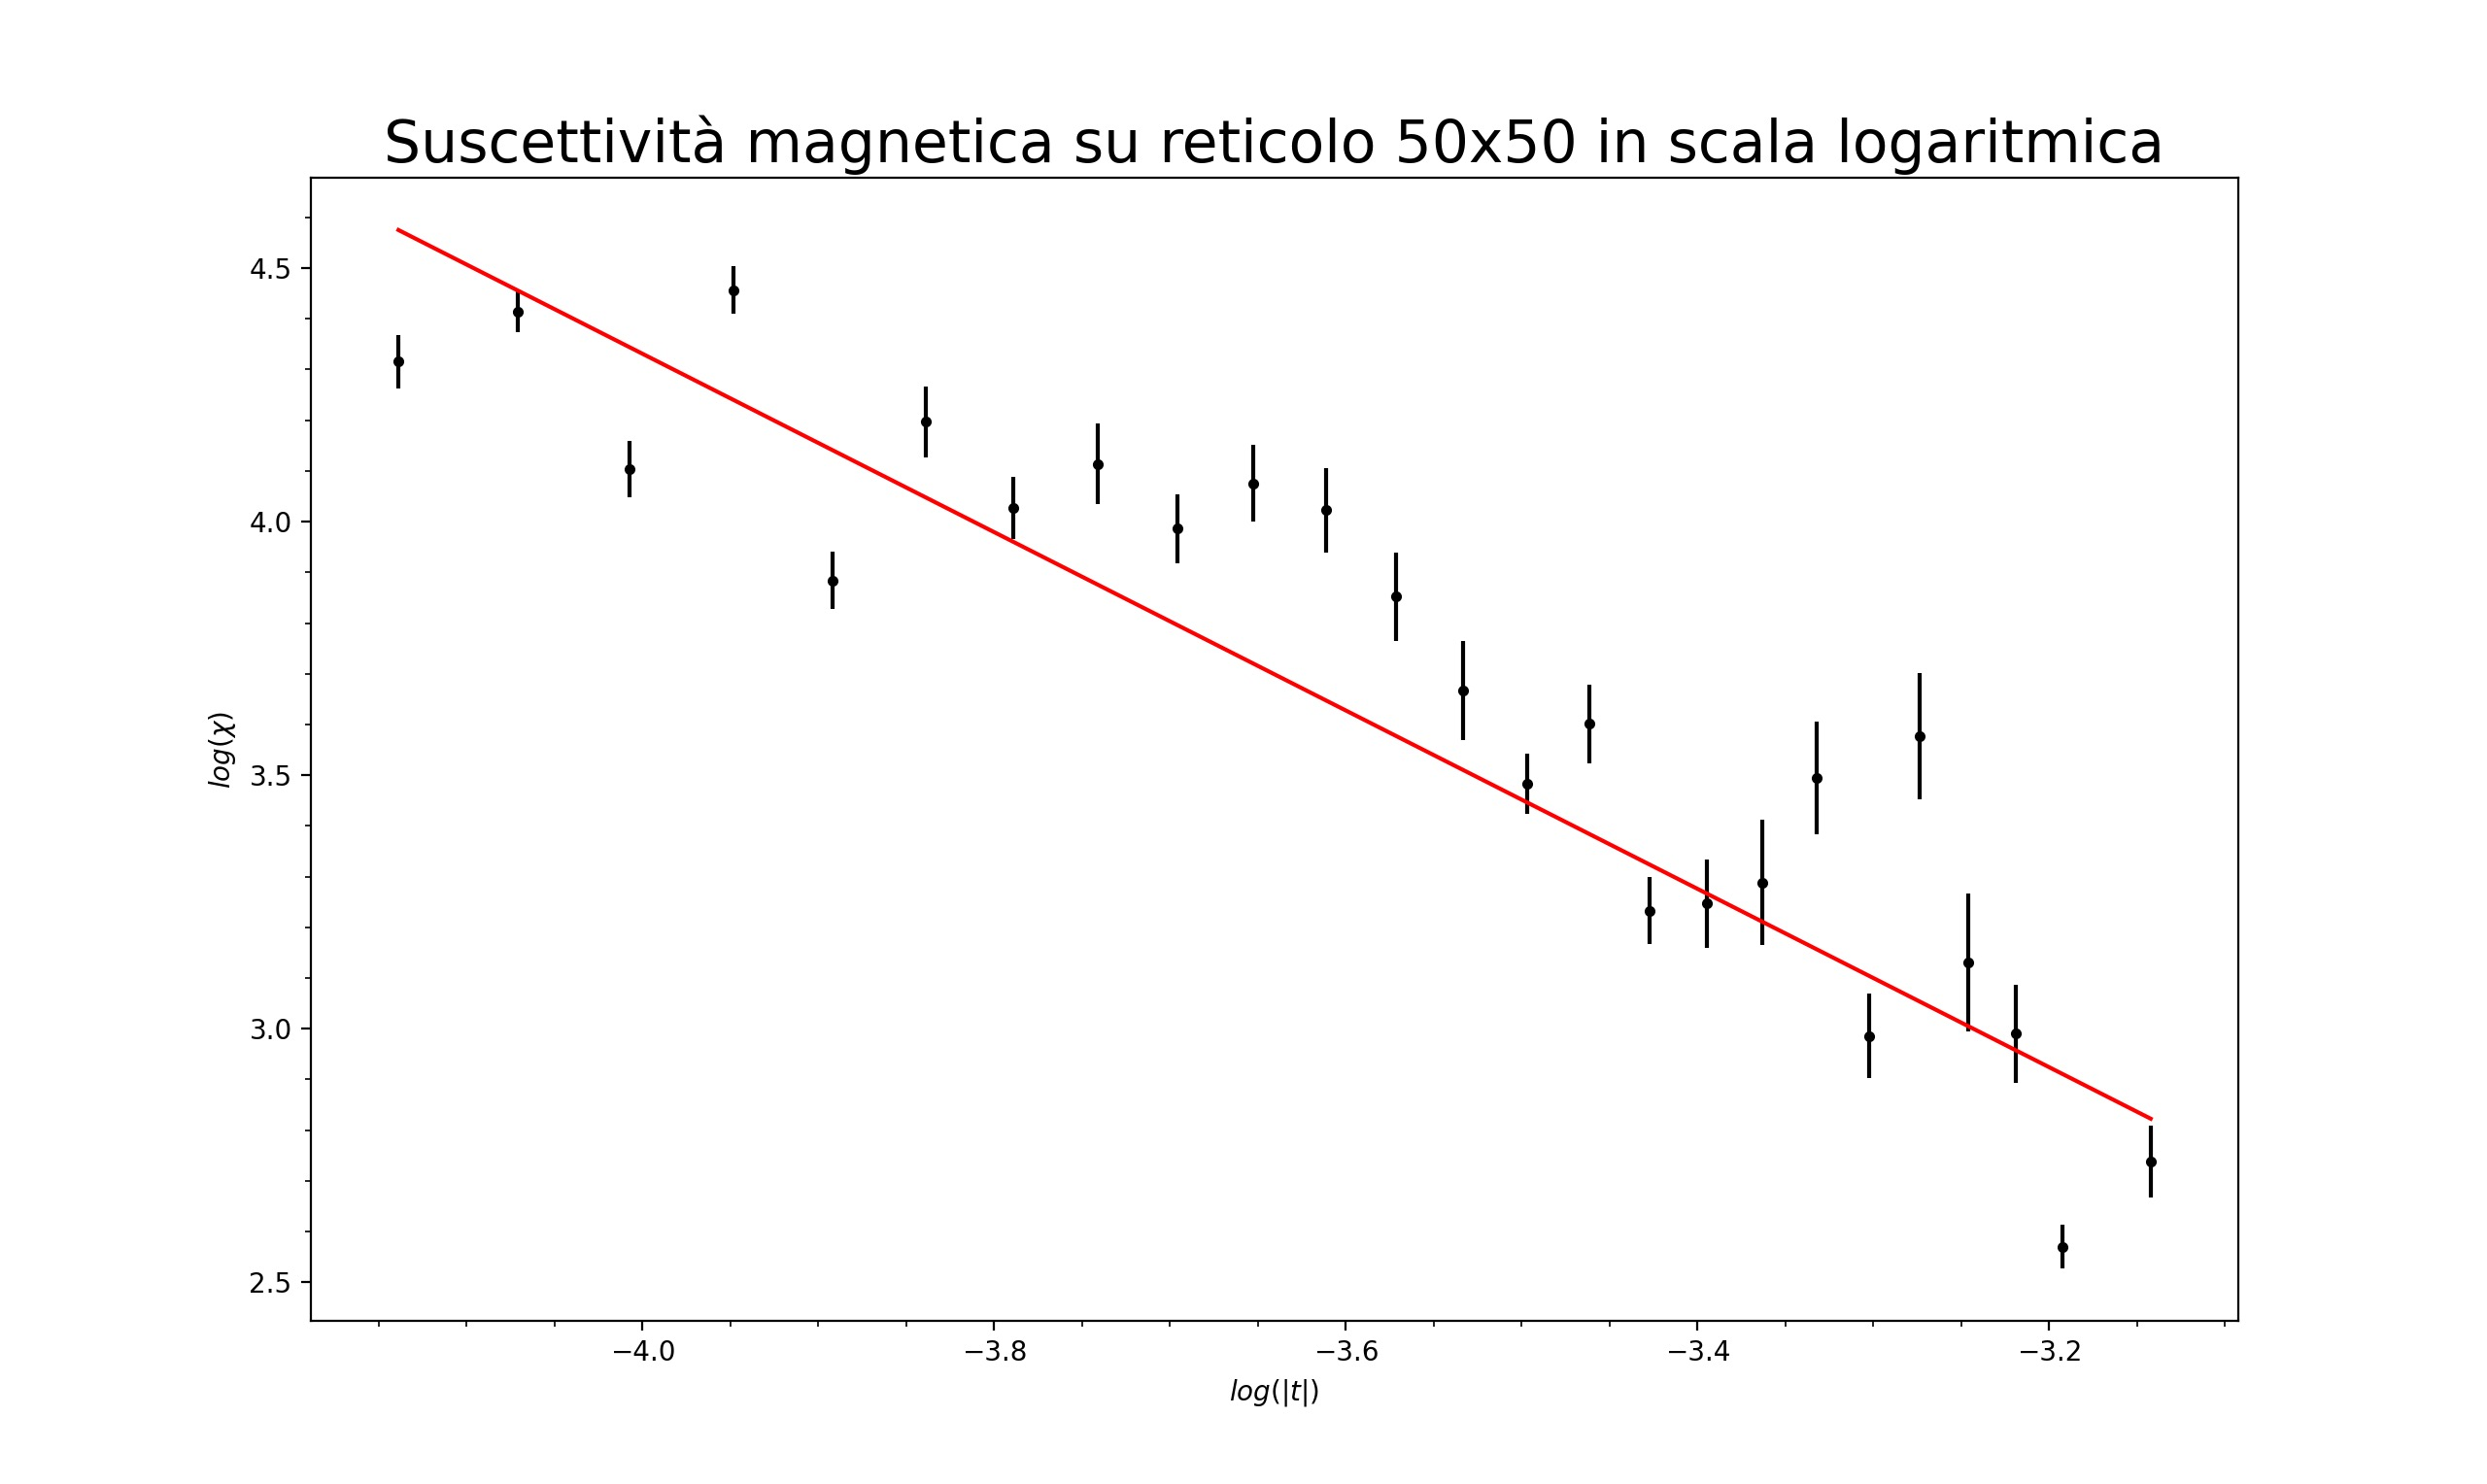
\includegraphics[width=1\linewidth]{gammadx}
	%\caption{Suscettività in funzione della temperatura ridotta in scala logaritmica. E' riportata anche la retta di best fit.}
	%\label{fig:gammadx}
%\end{figure}



\section{Comportamento ad alte e basse temperature}\label{CompAsint}
Il comportamento asintotico previsto è tale che per $T\rightarrow\infty$ la distribuzione di probabilità è all'incirca piatta sullo spazio delle configurazioni, mentre per $T\rightarrow 0$ le le configurazioni più probabili sono quelle con tutti spin up o con tutti spin down.
In figura \ref{beta01} vengono riportate tutte le osservabili di interesse per $L=10$ e campo magnetico esterno nullo.
\begin{figure}[h!]
	\centering
	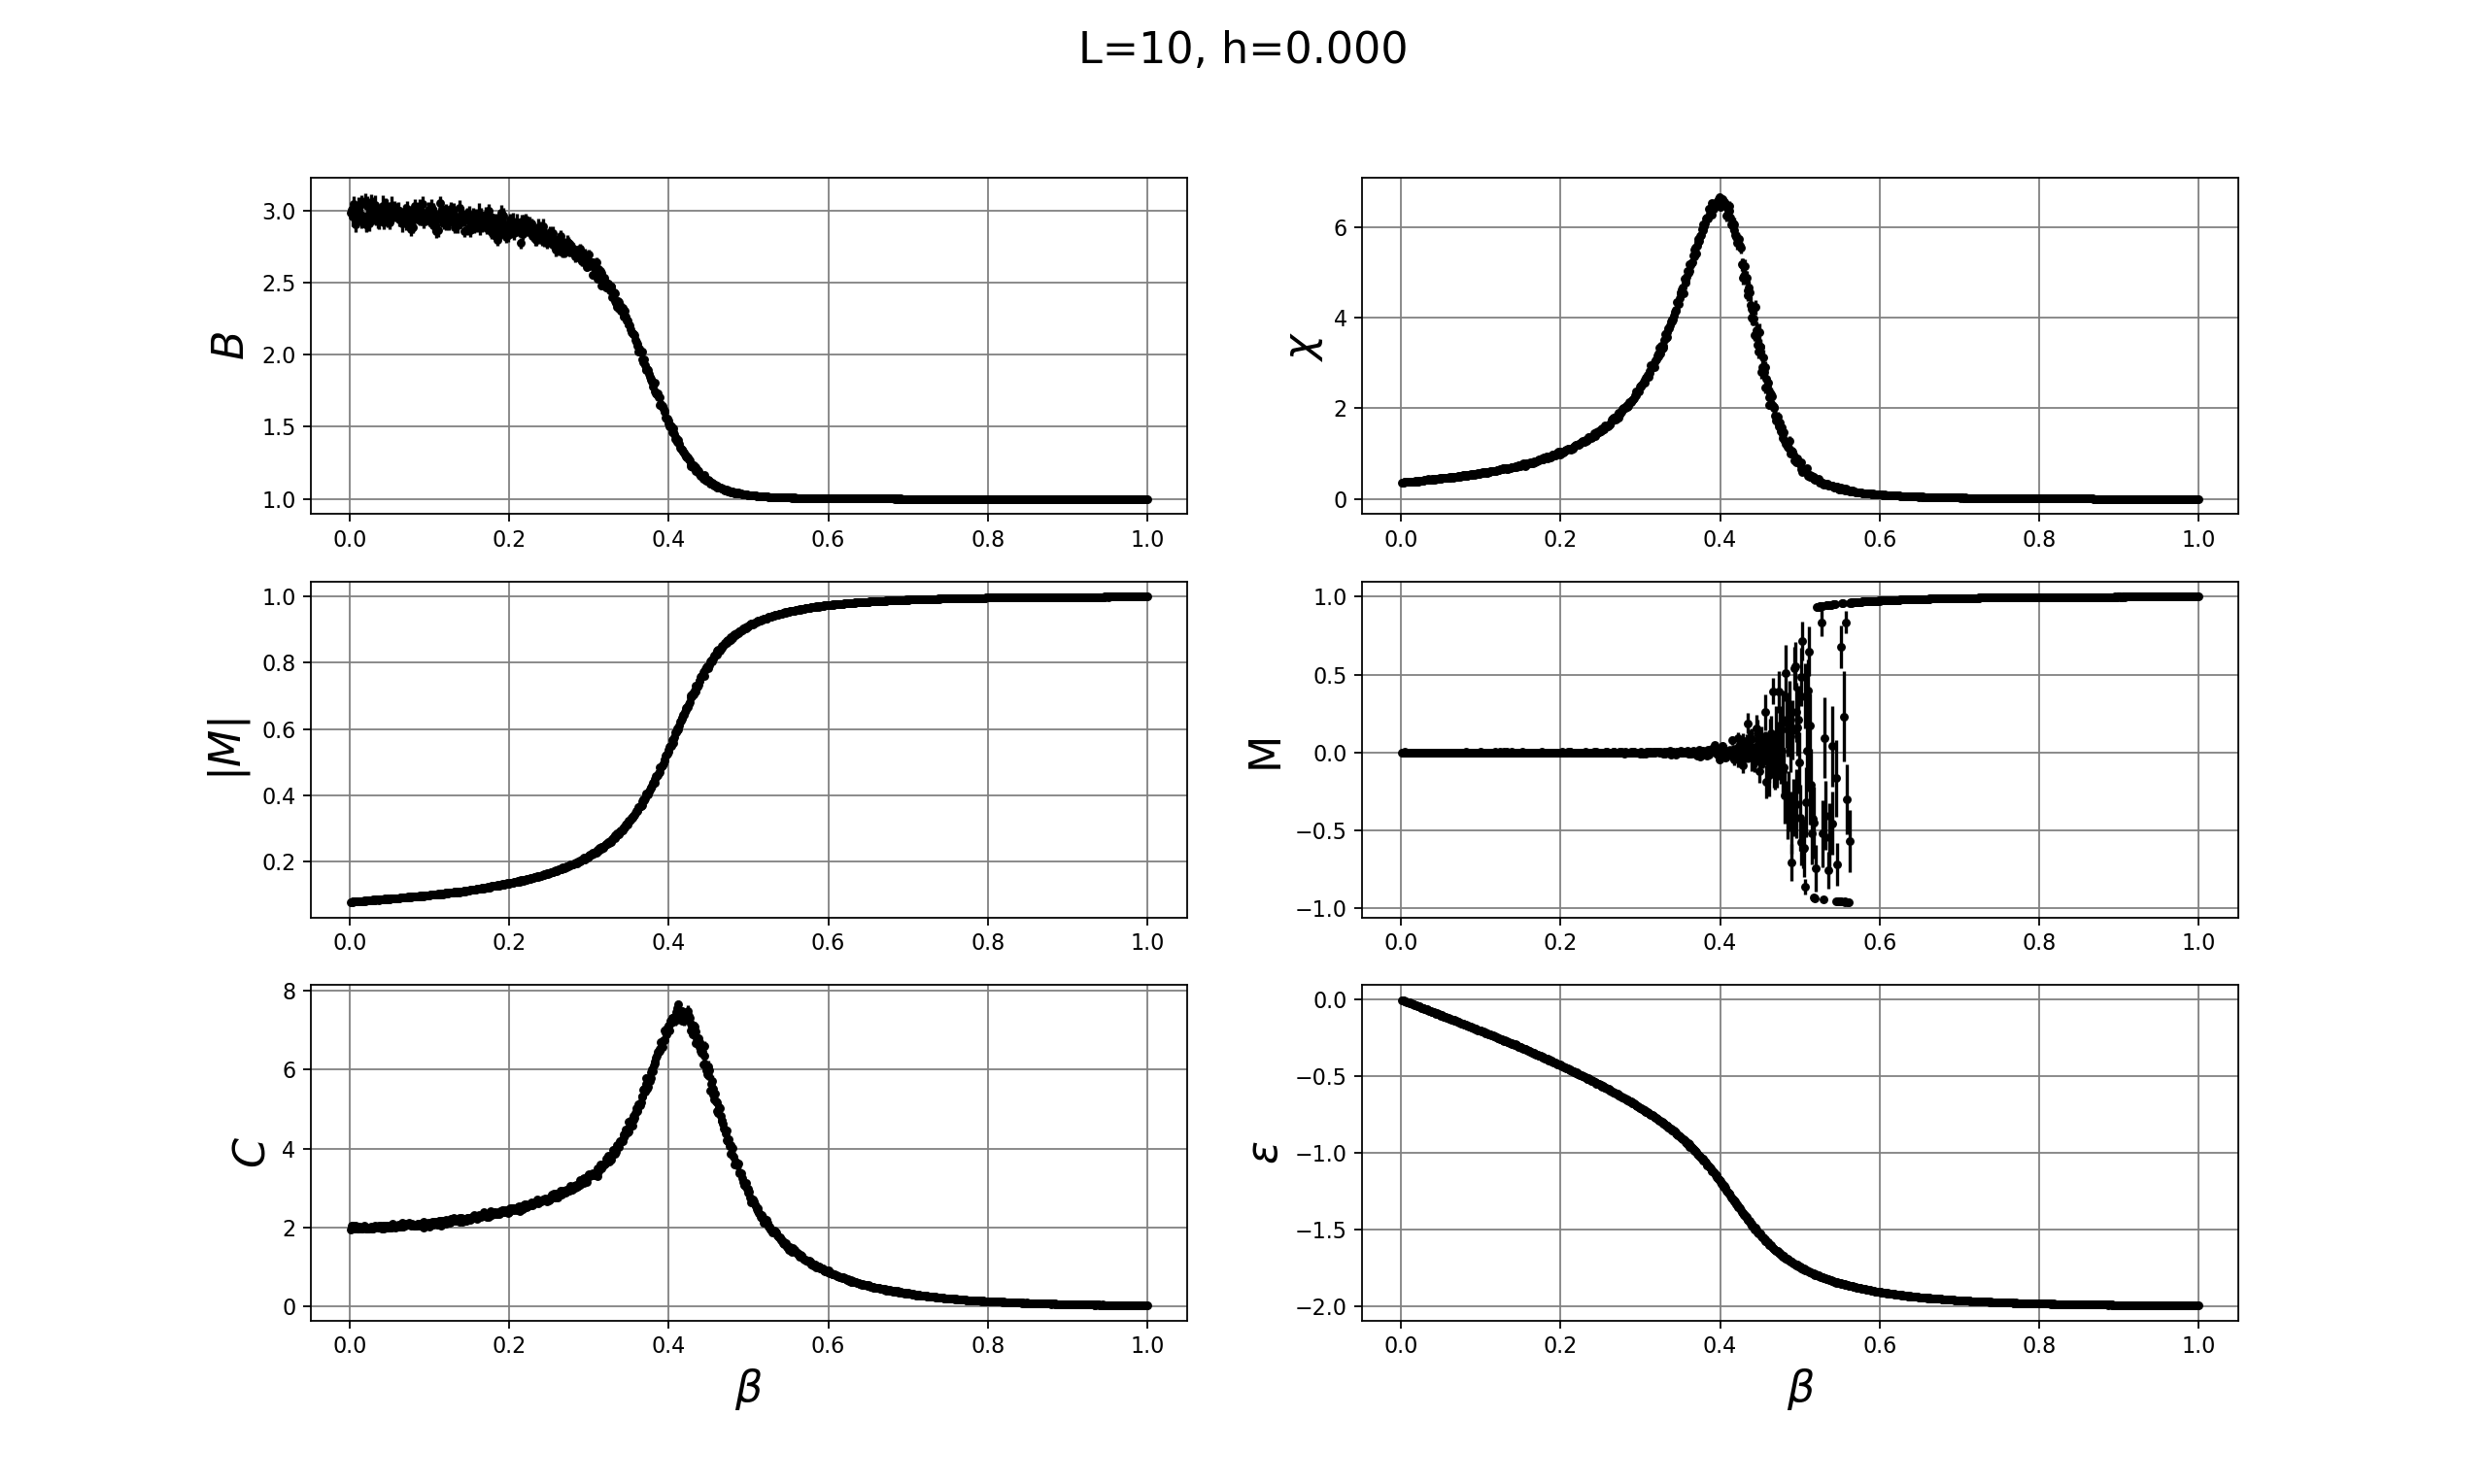
\includegraphics[width=1\linewidth]{beta01}
	\caption{Plot della suscettività, magnetizzazione, valore assoluto della magnetizzazione, calore specifico, cumulante di binder e energia per sito al variare di $\beta\in[0.001,1.000]$ a step di $\delta\beta=0.001$ per $L=10$ e $h=0$.}
	\label{beta01}
\end{figure}
Il comportamento asintotico rispetta le aspettative teoriche\footnote{Nel seguito con la parola "temperatura" intendiamo $T$ e non $\beta$.}:
\begin{itemize}
\item $B$ tende a 3 per alte temperature mentre tende a 1 per basse temperature, come atteso.
\item $|M|$ tende ad un valore piccolo ma diverso da 0 per alte temperature. Ciò è dovuto al valore assoluto. Mentre tende a 1 per basse temperature, come atteso.
\item $M$ tende a 0 per alte temperature, come atteso. Sopra la temperatura critica, invece, è diversa da $0$. Questo comportamento è legato al fatto che la storia montecarlo è composta da un numero di misure talmente basso che il sistema non riesce a far cambiare segno alla magnetizzazione. Se riuscissimo a fare simulazioni montecarlo con un numero sufficientemente grande di misure, allora $M$ deve valere $0$ entro l'incertezza.
\item $\chi$ tende ad un valore piccolo non nullo per alte temperature mentre tende a $0$ per basse temperature. Questo comportamento asintotico è legato a quello di $|M|$ (essendo $\chi$ proporzionale alla varianza di $|M|$).
\item $\epsilon$ tende all'energia per sito più bassa per temperature piccole (corrispondente alla configurazione con tutti spin up o tutti spin down) e ciò è in accordo con il terzo principio della termodinamica. Mentre per alte temperature tende a $0$, ovvero alla media aritmetica delle energie di tutte le configurazioni possibili, come atteso.
\item il comportamento di $C$ si spiega dal fatto che è proporzionale alla derivata di $\epsilon$ rispetto a $\beta$.

\end{itemize}
Ora analizziamo più nel dettaglio il comportamento per $\beta\rightarrow 0$  di $\langle\epsilon\rangle$ e di $C$. Si ha:
\begin{align*}
	&\langle\epsilon\rangle=\frac{1}{L^2}\sum_{\sigma}E[\sigma]\frac{e^{-\beta E[\sigma]}}{Z}=\frac{1}{L^2Z}\left(\sum_{\sigma}E[\sigma]-\beta\sum_{\sigma}E^2[\sigma]+O(\beta^2)\right)\\&=\frac{1}{L^2}\left(\frac{1}{\sum_{\sigma}1+O(\beta^2)}\right)\left(-\beta\sum_{\sigma}E^2[\sigma]+O(\beta^2)\right)=\\&=-\frac{\beta}{L^22^{L^2}}\sum_{\sigma}E^2[\sigma]+O(\beta^2)=-2\beta+O(\beta^2)
\end{align*}
dove è stato usato che nel caso di campo magnetico nulla risulta:
$$\sum_{\sigma}E[\sigma]=-\sum_{\langle s_i s_j\rangle}\sum_{\sigma}s_is_j=0$$
\begin{align*}
&\sum_{\sigma}E^2[\sigma]=\sum_{\langle s_i s_j\rangle}\sum_{\langle s_k s_l\rangle}\sum_{\sigma}s_is_js_ks_l=\sum_{\langle s_i s_j\rangle}\sum_{\sigma}(s_i)^2(s_j)^2=\\&=\sum_{\langle s_i s_j\rangle}\sum_{\sigma}1=2^{L^2}\sum_{\langle s_i s_j\rangle}1=2^{L^2}2L^2
\end{align*}
Inoltre, analogamente, risulta:
$$C=L^2\left[\langle\epsilon^2\rangle-\langle\epsilon\rangle^2\right]=L^2\left[\langle\epsilon^2\rangle+O(\beta^2)\right]=\frac{1}{L^22^{L^2}}\sum_{\sigma}E^2[\sigma]+O(\beta^2)=2+O(\beta^2)$$
Riassumendo:
$$\langle\epsilon\rangle=-2\beta+O(\beta^2)$$
$$C=2+O(\beta^2)$$
Ciò è in totale accordo con quanto si osserva in figura \ref{beta01}. Più nel dettaglio, in figura \ref{enebeta0} viene riportata l'energia in funzione di $\beta$ e la retta $f(\beta)=-2\beta$.

\begin{figure}[h!]
	\centering
	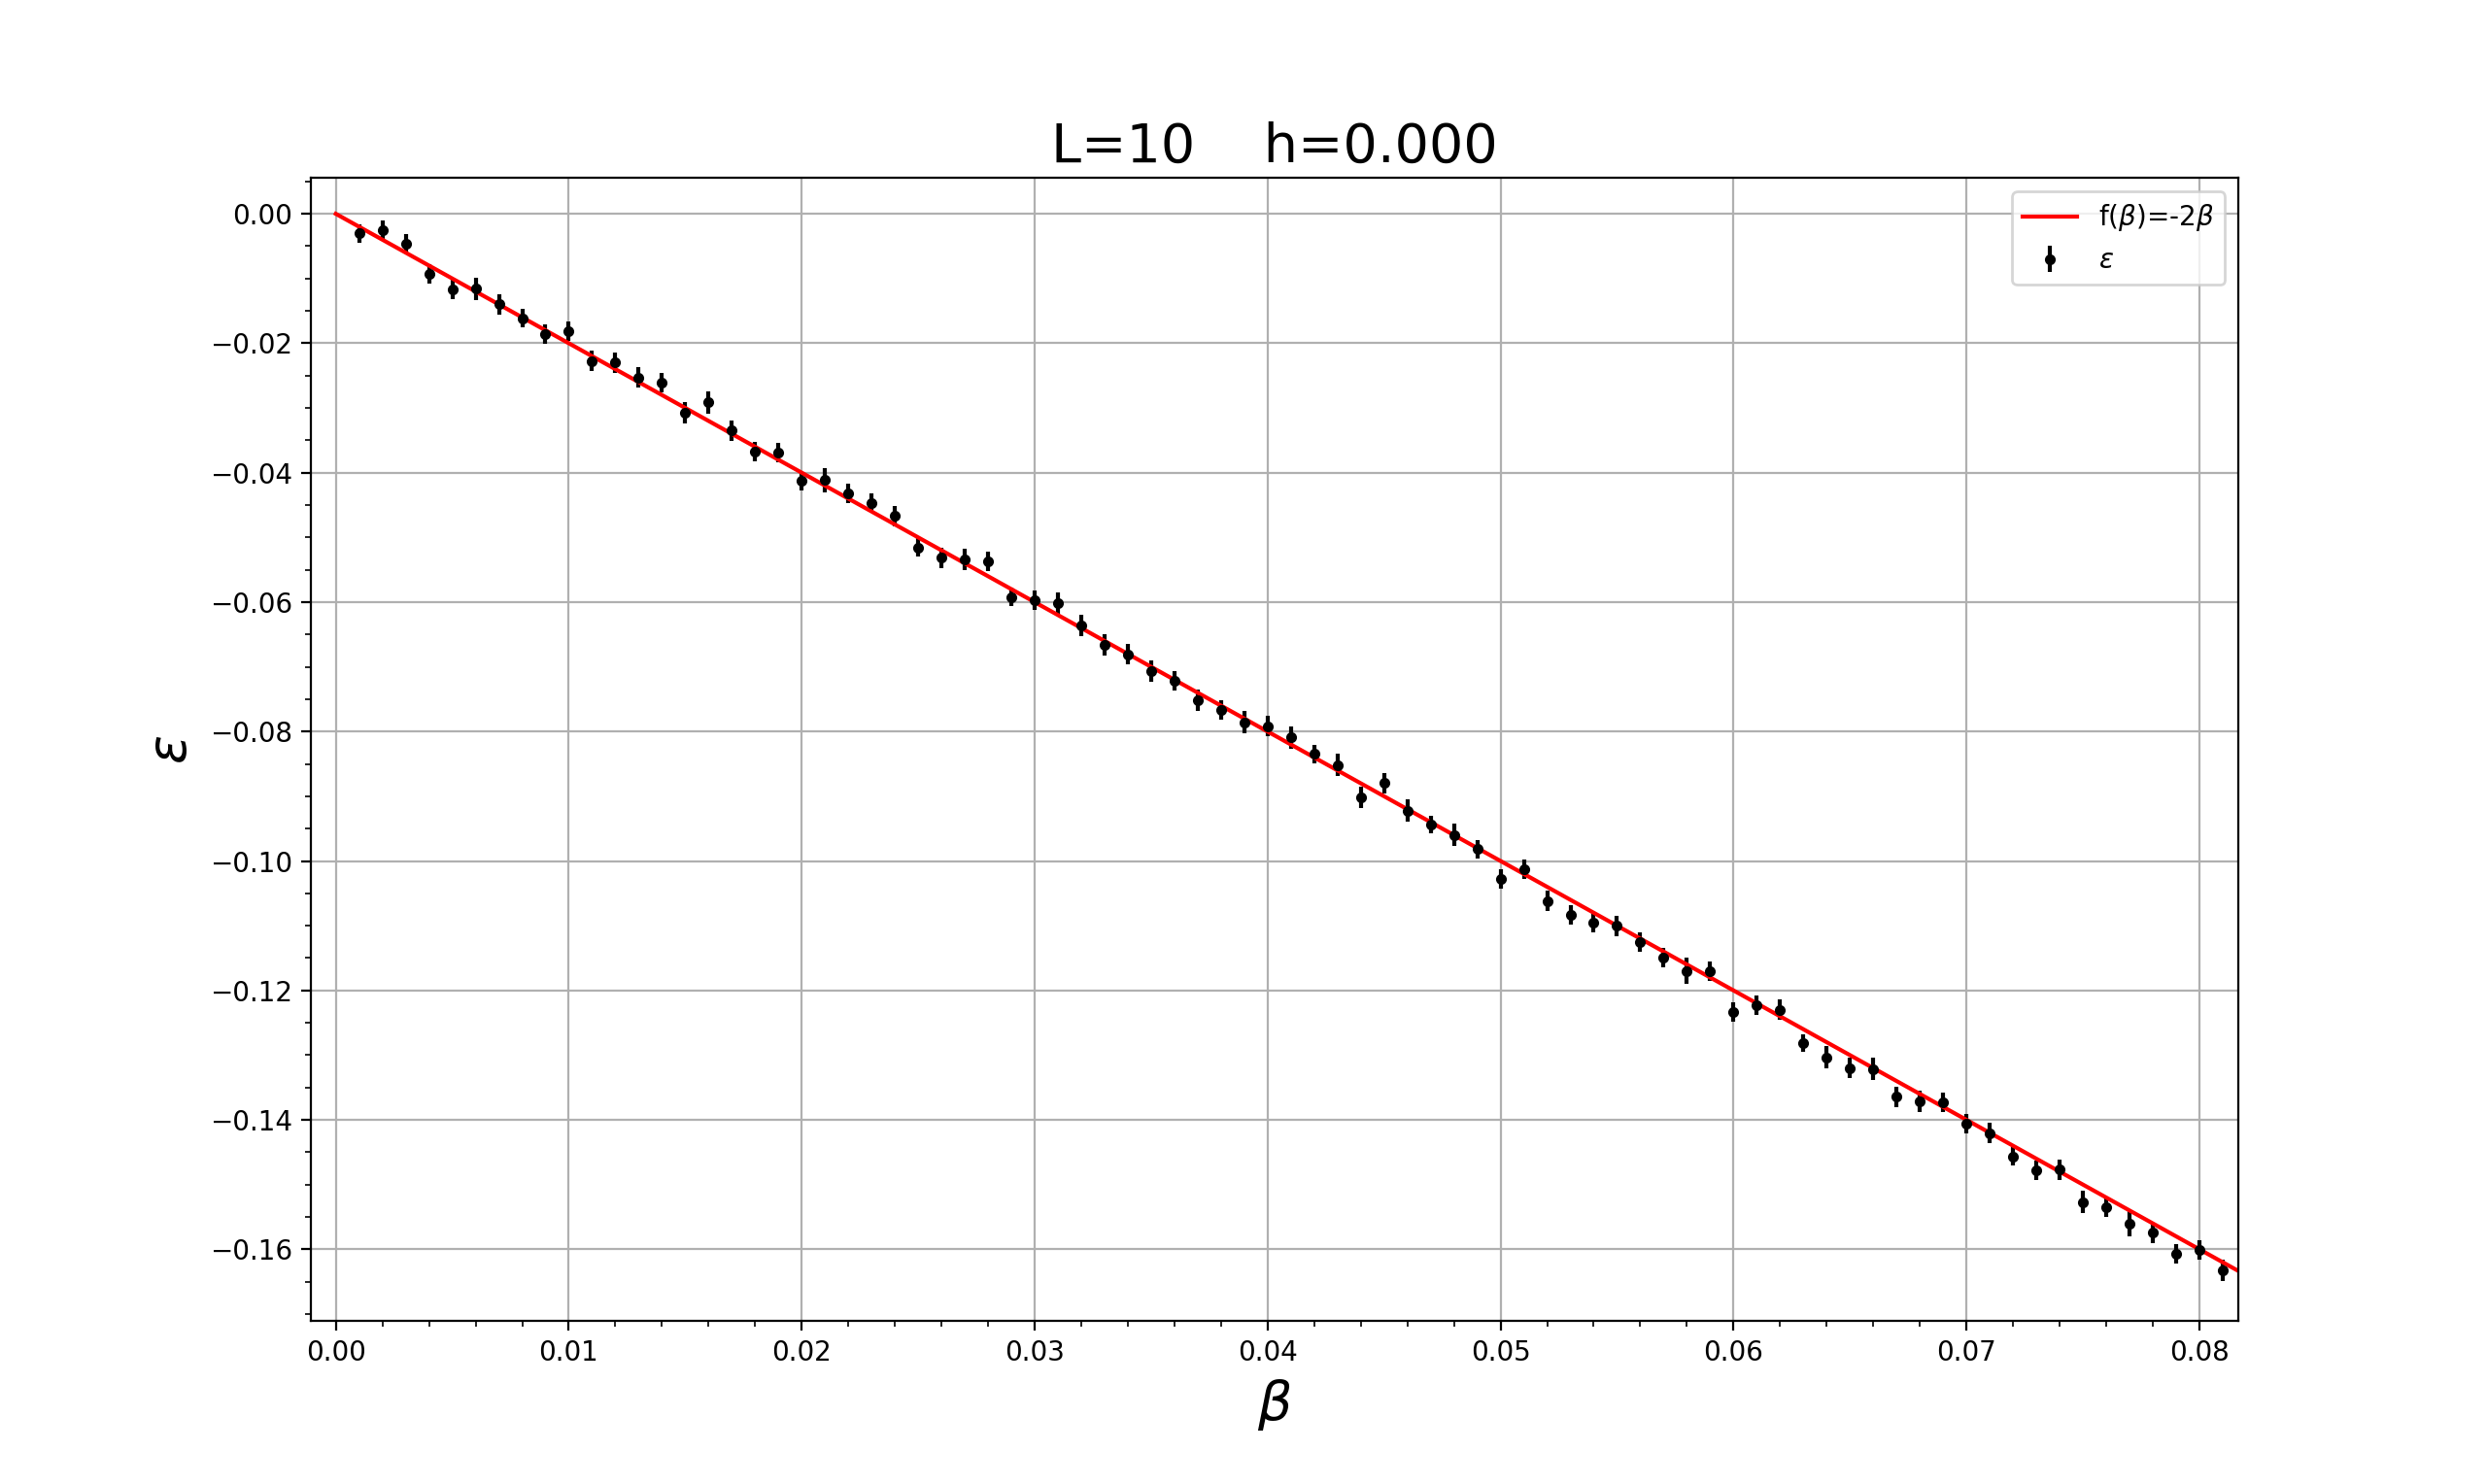
\includegraphics[width=1\linewidth]{enebeta0}
	\caption{Plot dell'energia per $\beta\in[0.001,0.080]$ a step di $\delta\beta=0.001$. Si osservi che vale $\langle\epsilon\rangle\sim -2\beta$ per $\beta$ piccolo.}
	\label{enebeta0}
\end{figure}




 

\section{Conclusioni}
E' stato simulato il modello di Ising classico 2D attraverso l'algoritmo Metropolis. E' stato calcolato il cumulante di Binder per vari $L$ in corrispondenza di $\beta=0.35$, $\beta=0.45$ e $\beta=0.50$, concludendo che $\beta=0.35$ corrisponde alla fase non rotta mentre $\beta=0.45$ e $\beta=0.50$ corrispondono alla fase rotta. E' stata calcolata la suscettività, il calore specifico, il valore assoluto della magnetizzazione, il cumulante di binder e l'energia per sito al variare di $\beta$ per alcuni $L$. Sono stati stimati gli indici critici $\nu$ e $\gamma$ (quest'ultimo è stato ricavato in due modi diversi), e la temperatura critica $\beta_c$. Tutte le stime numeriche ottenute sono in accordo con le previsioni teoriche. Inoltre, è stata ricavata la dipendenza del punto di massimo della suscettività al variare di $L$ (equazione \ref{eq:betapc}). Successivamente, è stata verificata l'ipotesi di scaling. Infine, è stato studiato il comportamento per alte e basse temperature. 
\newpage






\end{document}